\documentclass[12pt]{article}
\usepackage{float}
\usepackage[left=2cm, right=2cm]{geometry}
\usepackage{Layers}
\usepackage[utf8]{vietnam}
\usepackage{microtype}
\usepackage{blindtext}
\usepackage{enumitem}
\usepackage{setspace}
\usepackage[hidelinks]{hyperref}
\usepackage{amssymb}
\usepackage{xcolor}
\usepackage{minted}
\usepackage{longtable}
\usepackage{indentfirst}
\usepackage{fancyhdr}
\usepackage[backend=biber]{biblatex}
\addbibresource{bibliography.bib}

\usepackage{graphicx}
\setlength{\parindent}{0.5cm}
%---------------
\definecolor{dkgreen}{rgb}{0,0.6,0}
\definecolor{gray}{rgb}{0.5,0.5,0.5}
\definecolor{mauve}{rgb}{0.58,0,0.82}
\definecolor{LightGray}{gray}{0.9}
\usepackage{fancyhdr}
\pagestyle{fancy}
\lhead{Chủ đề: Tấn công Hệ mã đối xứng}

\rhead{Nhóm 5}
\rfoot{Trang \thepage}
\renewcommand{\headrulewidth}{0.4pt}
\renewcommand{\footrulewidth}{0.4pt}

\title{Mật mã và\\ độ phức tạp thuật toán}
\subtitle{Tấn công Hệ mã đối xứng }


\author{ \fontsize{13pt}{12pt}
\begin{tabular}{l l}
\textbf{Nhóm 5:} & \\
\textbf{Lê Nguyệt Hà} & \textbf{20216822}\\
\textbf{Nguyễn Thị Ngọc Hiền} & \textbf{20216826}\\
\textbf{Nguyễn Thị Trang} & \textbf{20216894}\\
\textbf{Đinh Minh Triều} & \textbf{20216895}\\
\textbf{Phạm Thị Thu Huê} & \textbf{20216832} \\[1cm]
\end{tabular}
}

% !TEX root = C:/báo cáo/main.tex
% \info{\textbf{GVHD: PGS.TS Nguyễn Đình Hân} \\
% }
\info{\fontsize{13pt}{12pt}
    \begin{tabular}{l l}
\textbf{GVHD:} & \textbf{PGS.TS Nguyễn Đình Hân} \\
 & \textbf{TS. Ngô Thị Hiền} \\
\end{tabular}
}

\usecolor{SamiBlue}
\flogo[width=0.45\textwidth]{logohustlong.png}
\slogo[width=0.48\textwidth]{fami xanh.png}

\begin{document}
\maketitlepage
\section*{Lời mở đầu}
\textbf{Bảo mật thông tin} là một vấn đề cấp bách trong kỷ nguyên số hóa hiện nay. Với sự phát triển của công nghệ, các cuộc tấn công mạng ngày càng tinh vi và nguy hiểm, đe dọa nghiêm trọng đến sự an toàn của dữ liệu và hệ thống. Trong số các phương thức bảo mật thông tin, mã hóa đóng vai trò quan trọng trong việc bảo vệ thông tin nhạy cảm khỏi những kẻ tấn công.\\
\indent \textbf{Mã hóa đối xứng} là một trong những phương pháp mã hóa phổ biến, sử dụng cùng một khóa để mã hóa và giải mã dữ liệu. Loại mã hóa này được sử dụng rộng rãi trong nhiều ứng dụng, từ bảo mật mạng đến bảo vệ dữ liệu cá nhân. Tuy nhiên, tấn công hệ mã đối xứng vẫn là một mối đe dọa tiềm ẩn, có thể khai thác lỗ hổng bảo mật của các thuật toán mã hóa và gây thiệt hại nghiêm trọng.\\
\indent Báo cáo này sẽ tập trung vào việc phân tích tấn công hệ mã đối xứng, đặc biệt là với hai thuật toán phổ biến là DES và AES-128. Báo cáo sẽ đề cập đến các phương pháp tấn công phổ biến như Brute Force, MITM,... và các biện pháp phòng chống tấn công. Ngoài ra, báo cáo sẽ trình bày một số mô phỏng tấn công thực tế để minh họa cho nguy cơ của các lỗ hổng bảo mật trong hệ mã đối xứng.\\
\newline
Nội dung chính của báo cáo bao gồm:
\begin{itemize}
    \item Giới thiệu về Hệ mật khóa đối xứng.
    \item Nguyên lý hoạt động và các thuật toán phổ biến như DES, AES.
    \item Phân tích các phương pháp tấn công: Brute Force, MITM,..., Tấn công Vi phân, Tấn công Tuyến tính và các biện pháp phòng tránh bị mất mát thông tin bởi các cuộc tấn công.
    \item Mô phỏng thuật toán DES, AES và tấn công Brute Force.
    \item Kết luận: Tổng kết những việc đã làm được và hướng nghiên cứu, phát triển trong tương lai.
\end{itemize}
\indent Báo cáo này nhằm mục đích nâng cao nhận thức về nguy cơ tấn công hệ mã đối xứng và cung cấp kiến thức cơ bản để bảo vệ dữ liệu khỏi những mối đe dọa tiềm ẩn.\\
\newline
\indent Thay mặt cả nhóm, em xin phép gửi lời cảm ơn đến PGS.TS Nguyễn Đình Hân và TS. Ngô Thị Hiền đã giảng dạy và hỗ trợ chúng em trong suốt quá trình hoàn thiện báo cáo. Nhờ những chỉ dẫn tận tình của thầy cô, nhóm chúng em đã mở rộng kiến thức và kỹ năng, cũng như áp dụng những lý thuyết này vào việc giải quyết những vấn đề cụ thể trong học tập. Bài báo cáo này sự cống gắng hết mình của cả nhóm tuy nhiên không thể tránh được sự sai sót. Chúng em hy vọng sẽ nhận được sự góp ý quý báu của thầy cô để hoàn thiện hơn nữa công trình nghiên cứu này.\\

    
    \hspace{10cm} \textbf{Nhóm trưởng}
    
    \vspace{20pt}
    \hspace{9.7cm} \textbf{Đinh Minh Triều}
\newpage
\setlength{\leftmargin}{-0.5mm}\tableofcontents

\section*{Đóng góp của thành viên}
\addcontentsline{toc}{section}{Đóng góp của thành viên}
\begin{tabular}{|p{3cm}|p{2cm}|p{11cm}|}
    \hline
    Thành viên & MSSV & Đóng góp\\ \hline
    Lê Nguyệt Hà & 20216822 & Giới thiệu về hệ mật khoá đối xứng, tìm hiểu mặt hạn chế của thuật toán AES, DES, tìm hiểu về tấn công Dictionary, khái niệm, mục đích, nguyên nhân tấn công Brute Force, viết báo cáo.\\ \hline
    Nguyễn Thị Ngọc Hiền & 20216826 & Tìm hiểu thuật toán DES, quá trình mã hóa AES, phương pháp tấn công Brute Force, phương pháp tấn công MITM, phương pháp tấn công KPA, phương pháp tấn công CPA, phương pháp tấn công Timing Attack, viết báo cáo.\\ \hline
   Nguyễn Thị Trang & 20216894 & Xây dựng chương trình mô phỏng Mã hóa và Giải mã hệ mật DES, chương trình mô phỏng tấn công hệ mật DES bằng phương pháp Brute Force, hỗ trợ lên ý tưởng nội dung, soạn slide, viết báo cáo. \\ \hline
    Phạm Thị Thu Huê & 20216832 & Tìm hiểu quá trình giải mã của thuật toán AES; xây dựng mô phỏng và lập trình phần mã hóa và giải mã bằng thuật toán AES; tìm hiểu các biện pháp bảo vệ trước các kĩ thuật tấn công như Brute Force, MITM, KPA, CPA, Timing; tìm hiểu một số hướng nghiên cứu và phát triển trong tương lai, viết báo cáo. \\ \hline
    Đinh Minh Triều & 20216895  & Giới thiệu về Tấn công Vi phân và Tấn công Tuyến tính, Hỗ trợ phần lập trình mô phỏng, lập kế hoạch và theo dõi tiến độ làm việc của nhóm, viết báo cáo.  \\
    \hline
\end{tabular}

\section{Giới thiệu về Hệ mật khoá đối xứng}
\subsection{Khái niệm về Mã khoá đối xứng}
Hệ mật khóa đối xứng (Symmetric Key Cryptography) là một phương pháp mã hóa trong đó cùng một khóa được sử dụng cho cả quá trình mã hóa và giải mã dữ liệu. Đây là một trong những kỹ thuật cơ bản và quan trọng trong lĩnh vực mật mã học, được sử dụng để đảm bảo tính bảo mật và toàn vẹn của thông tin \cite{galil1986symmetric}.
   \begin{figure}[H]
    \centering
    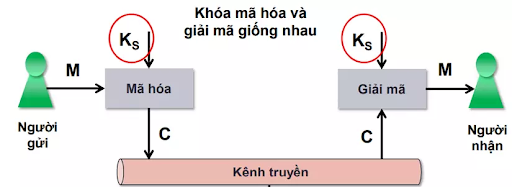
\includegraphics[scale=0.6]{pic/kn_mmdx.png}
    \caption{ Mô hình mã hoá, giải mã bằng khoá đối xứng}
    
\end{figure}
    


\subsection{Ứng dụng của hệ mật khoá đối xứng}
\begin{itemize}
    \item \textbf{Mã hóa dữ liệu}
    \begin{itemize}
        \item  Hệ mật khóa đối xứng được sử dụng để mã hóa dữ liệu lưu trữ trên các thiết bị hoặc cơ sở dữ liệu nhằm bảo vệ thông tin nhạy cảm khỏi truy cập trái phép.
        \item AES (Advanced Encryption Standard) thường được sử dụng để mã hóa dữ liệu trong các hệ thống lưu trữ thông tin quan trọng, như dữ liệu tài chính hoặc y tế.
    \end{itemize}

    \item \textbf{Bảo mật kênh truyền thông}
    \begin{itemize}
        \item  Bảo mật các kênh truyền thông giữa hai hoặc nhiều bên để đảm bảo rằng thông tin truyền tải không bị nghe trộm hoặc thay đổi.
        \item Giao thức SSL/TLS sử dụng mã hóa đối xứng để bảo vệ các kết nối HTTPS, đảm bảo an toàn cho giao dịch ngân hàng trực tuyến, email, và mua sắm trực tuyến.
    \end{itemize}

    \item \textbf{Bảo mật mạng không dây}
    \begin{itemize}
        \item  Mã hóa lưu lượng mạng để bảo vệ dữ liệu truyền qua mạng không dây khỏi bị nghe trộm.
        \item  Các giao thức bảo mật mạng không dây như WPA2 (Wi-Fi Protected Access II) sử dụng mã hóa đối xứng để bảo vệ thông tin truyền qua mạng Wi-Fi.
    \end{itemize}

    \item \textbf{Bảo vệ ổ đĩa và thiết bị lưu trữ}
    \begin{itemize}
        \item  Mã hóa toàn bộ ổ đĩa hoặc thiết bị lưu trữ để bảo vệ dữ liệu nếu thiết bị bị mất hoặc bị đánh cắp.
        \item  BitLocker của Microsoft sử dụng AES để mã hóa toàn bộ ổ đĩa trên hệ điều hành Windows, bảo vệ dữ liệu trong trường hợp mất mát hoặc trộm cắp thiết bị.
    \end{itemize}

    \item \textbf{Bảo mật ứng dụng và dịch vụ đám mây}
    \begin{itemize}
        \item  Mã hóa dữ liệu được lưu trữ và truyền tải qua các dịch vụ đám mây để đảm bảo tính bảo mật và riêng tư của thông tin.
        \item  Các dịch vụ đám mây như Amazon Web Services (AWS) và Google Cloud Platform (GCP) cung cấp các tùy chọn mã hóa đối xứng cho dữ liệu lưu trữ trong đám mây.
    \end{itemize}

    \item \textbf{Mã hóa tin nhắn}
    \begin{itemize}
        \item  Bảo mật tin nhắn trao đổi giữa người dùng qua các ứng dụng nhắn tin tức thời.
        \item  Nhiều ứng dụng nhắn tin như WhatsApp sử dụng mã hóa đầu-cuối (End-to-End Encryption), một dạng mã hóa đối xứng để bảo vệ nội dung tin nhắn khỏi bị đọc trộm.
    \end{itemize}
\end{itemize}
\subsection{Ưu điểm của Hệ mật khóa đối xứng}

\begin{itemize}
    \item \textbf{Tốc độ và hiệu quả}
    \begin{itemize}
        \item  Hệ mật khóa đối xứng sử dụng các thuật toán đơn giản hơn so với hệ mật khóa bất đối xứng, dẫn đến tốc độ mã hóa và giải mã nhanh hơn.
        \item  Điều này làm cho nó phù hợp với các ứng dụng yêu cầu xử lý dữ liệu lớn hoặc yêu cầu thời gian thực, chẳng hạn như mã hóa dữ liệu trên đĩa, truyền thông thời gian thực, và các giao dịch trực tuyến.
    \end{itemize}

    \item \textbf{Đơn giản trong triển khai}
    \begin{itemize}
        \item Các thuật toán mã hóa đối xứng dễ hiểu và dễ triển khai.
        \item Do sự đơn giản của các thuật toán như AES và DES, việc triển khai và tích hợp chúng vào các hệ thống bảo mật dễ dàng hơn. Điều này giúp giảm thiểu lỗi trong quá trình triển khai và duy trì.
    \end{itemize}

    \item \textbf{Tiết kiệm tài nguyên}
    \begin{itemize}
        \item Hệ mật khóa đối xứng tiêu thụ ít tài nguyên hệ thống hơn so với hệ mật khóa bất đối xứng.
        \item  Do tính chất đơn giản của các thuật toán, chúng tiêu thụ ít CPU và bộ nhớ hơn, làm cho nó trở thành lựa chọn lý tưởng cho các thiết bị có tài nguyên hạn chế như điện thoại di động, thiết bị IoT, và các hệ thống nhúng.
    \end{itemize}

    \item \textbf{Bảo mật dữ liệu Tốt}
    \begin{itemize}
        \item Khi được sử dụng đúng cách với một khóa đủ mạnh và bảo mật, hệ mật khóa đối xứng cung cấp mức độ bảo mật rất cao.
        \item  Các thuật toán như AES hiện tại được coi là rất an toàn và chưa có phương pháp tấn công hiệu quả nào có thể phá vỡ chúng trong thời gian hợp lý, nếu khóa được bảo mật tốt.\cite{agrawal2012comparative}
    \end{itemize}

    \item \textbf{Khả năng Tương thích}
    \begin{itemize}
        \item  Hệ mật khóa đối xứng tương thích tốt với nhiều giao thức và tiêu chuẩn bảo mật hiện tại.
        \item  Nó được tích hợp vào nhiều giao thức bảo mật như SSL/TLS cho bảo mật web, IPsec cho mạng, và WPA2 cho mạng không dây, làm cho nó dễ dàng tích hợp vào các hệ thống hiện có.
    \end{itemize}
\end{itemize}

\subsection{ Mặt hạn chế của hệ mật khoá đối xứng}
\begin{itemize}
    \item \textbf{Phân phối khóa}
    \begin{itemize}
        \item  Để hệ mật khóa đối xứng hoạt động, cả người gửi và người nhận phải có cùng một khóa mật. Việc phân phối khóa này phải được thực hiện qua một kênh an toàn, nếu không khóa có thể bị đánh cắp.
        \item Quá trình trao đổi khóa an toàn là một thách thức lớn, đặc biệt trong các mạng lớn hoặc các hệ thống với nhiều người dùng \cite{alenezi2020symmetric}.
    \end{itemize}

    \item \textbf{Quản lý khóa}
    \begin{itemize}
        \item Trong một hệ thống có nhiều người dùng, số lượng khóa cần quản lý tăng lên rất nhanh, do mỗi cặp người dùng cần có một khóa riêng biệt.
        \item  Với \( n \) người dùng, số lượng khóa cần quản lý là \( \frac{n(n-1)}{2} \), điều này dẫn đến sự phức tạp và khó khăn trong việc lưu trữ và quản lý khóa an toàn.
    \end{itemize}

    \item \textbf{Không hỗ trợ xác thực}
    \begin{itemize}
        \item  Hệ mật khóa đối xứng không hỗ trợ cơ chế xác thực nguồn gốc của thông tin.
        \item Vì cả hai bên đều sử dụng cùng một khóa, không có cách nào để xác minh ai là người thực hiện quá trình mã hóa. Điều này làm cho việc xác thực và đảm bảo tính toàn vẹn của thông tin trở nên khó khăn.
    \end{itemize}

    \item \textbf{Không bảo mật trước các cuộc tấn công nhân bản}
    \begin{itemize}
        \item Nếu khóa mật bị đánh cắp, kẻ tấn công có thể mã hóa và giải mã thông tin, gây nguy hiểm cho toàn bộ hệ thống.
        \item Một khi khóa bị lộ, tất cả các thông tin đã mã hóa bằng khóa đó có thể bị giải mã, dẫn đến mất mát dữ liệu và vi phạm an ninh.
    \end{itemize}

    \item \textbf{Thiếu linh hoạt so với hệ mật khóa bất đối xứng}
    \begin{itemize}
        \item Hệ mật khóa đối xứng không linh hoạt bằng Hệ mật khóa bất đối xứng (Asymmetric Key Cryptography).
        \item Hệ mật khóa bất đối xứng sử dụng một cặp khóa công khai và khóa riêng, giúp giải quyết nhiều vấn đề phân phối khóa và xác thực, mặc dù có tốc độ chậm hơn.
    \end{itemize}
\end{itemize}

\section {Các Hệ mã khóa đối xứng nổi tiếng}
\subsection{Thuật toán DES}
\subsubsection{Lịch sử hình thành}
\begin{itemize}
    \item Thuật toán mã khối DES (Data Encryption Standard) là một thuật toán mã khối với kích thước khối 64 bít và kích thước khóa 56 bít, được công bố chính thức bởi Tổ chức Tiêu chuẩn xử lý thông tin liên bang Hoa Kỳ (FIPS) vào tháng 11/1976 và được xuất bản trong tài liệu FIPS PUB 46 (01/1977) \cite{Khanh2014}.
    \item Tiền thân của thuật toán DES là thuật toán Lucifer, một thuật toán do IBM phát triển. Cuối năm 1976, DES được chọn làm chuẩn mã hóa dữ liệu của Hoa Kỳ, sau đó được sử dụng rộng rãi trên toàn thế giới trong lĩnh vực an toàn, bảo mật thông tin trên môi trường số \cite{Khanh2014}.
\end{itemize}
\subsubsection{Thuật toán và lưu đồ hoạt động mã hóa dữ liệu DES}
\begin{itemize}
    \item Input: Khối độ dài 64 bits và khóa là 56 bits.
    \item Output: Đầu ra 64 bits.
    \begin{figure}[H]
        \centering
        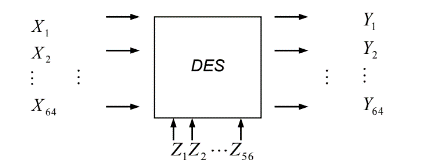
\includegraphics{D:/trang/mật mã/báo cáo/Ảnh/hiền/lưu đồ des.png}
        \caption{Lưu đồ hoạt động DES}
    \end{figure}
\end{itemize}
Thuật toán DES được sử dụng để mã hóa và giải mã các block (khối) dữ liệu 64 bit dựa trên một key (khóa mã) 64 bit.\\
\underline{Chú ý:}  Các block được đánh số thứ tự bít từ trái sang phải và bắt đầu từ 1, bit đầu tiên bên trái là bit số 1 và bit cuối cùng bên phải là bit số 64.\\
\indent Quá trình giải mã và mã hóa sử dụng cùng một key nhưng thứ tự phân phối các giá trị các bit key của quá trình giải mã ngược với quá trình mã hóa.
DES được cấu tạo bởi 16 bước lặp với bước lặp cơ sở gọi hàm chuyển đổi phi tuyến $f$ (có thể hiểu là việc tính toán dựa trên key); 16 bước lặp này được kẹp vào giữa hai tác tử giao hóa IP và IP$^{-1}$. Một block dữ liệu sẽ được hóan vị khởi tạo (Initial Permutation) IP trước khi thực hiện tính toán mã hóa với key, cuối cùng kết quả tính toán với key sẽ được hóa vị lần nữa - đây là hoán vị đảo của hoán vị khởi tạo được gọi là IP$^{-1}$. Hàm cơ sở $f$ là nguồn gốc của sức mạnh bảo mật trong thuật toán DES. Sự lặp lại nhiều lần các bước lặp với tác dụng của f là nhằm tăng cường \textbf{tính nhập nhằng và khuếch tán} (Confusion \& Diffusion) đã có trong $f$.
Hàm $KS$, gọi là hàm phân phối key (Key Schedule). Đây là hàm tạo ra các khóa vòng (Round Key) cho các lần lặp mã hóa. Có tất cả 16 khóa vòng từ $K_1$ đến $K_{16}$ \cite{Khanh2014}.
\begin{figure}[H]
    \centering
    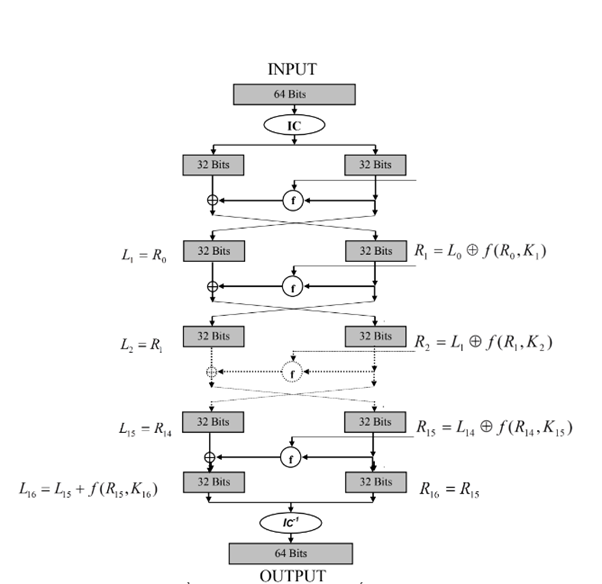
\includegraphics[width=\textwidth,height=15cm]{D:/trang/mật mã/báo cáo/Ảnh/hiền/lưu đồ des-1.png}
    \caption{Sơ đồ sinh mã DES}
\end{figure}
Trên đây là sơ đồ sinh mã DES với cấu trúc 16 vòng lặp.
\subsubsection{Hoán vị khởi tạo - $IP$}
Hoán vị là thay đổi vị trí các bit trong một chuỗi giá trị nhưng không làm thay đổi giá trị của các bit này. Đây là bước đầu tiên trong quy trình mã hóa dữ liệu. 64 bit dữ liệu đầu vào, gọi là Plaintext, sẽ được hoán vị theo bảng mô tả sau đây.
\begin{figure}[H]
    \centering
    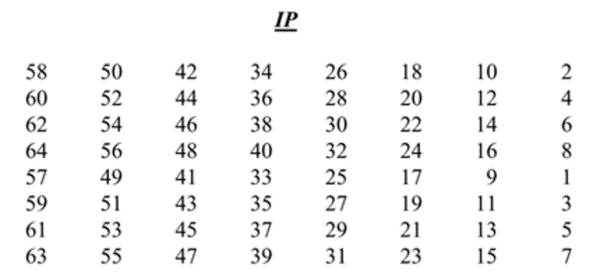
\includegraphics[width=\textwidth]{D:/trang/mật mã/báo cáo/Ảnh/hiền/IP.png}
    \caption{Bảng tra cứu $IP$}
\end{figure}
\indent Chuỗi bit đầu vào được đánh số từ 1 đến 64 (tính từ trái qua phải). Sau đó, các bit này được thay đổi vị trí như sơ đồ $IP$, bit số 58 được đặt vào vị trí đầu tiên, bit số 50 được đặt vào vị trí thứ 2. Cứ như vậy, bit thứ 7 được đặt vào vị trí cuối cùng.\\
\indent Sau hoán vị, chuỗi bit mới được phân ra làm hai đoạn, mỗi đoạn 32 bit để bắt đầu vào quy trình tính toán mã hóa với key. 
\begin{itemize}
    \item Đoạn bên trái kí hiệu là $L$: gồm các bit từ bit số 1 đến bit số 32.
    \item Đoạn bên phải kí hiệu là $R$: các bit từ bit số 33 đến bit số 64.
    \item Đoạn $L$ của lần tính toán sau sẽ chính là đoạn $R$ của lần tính toán trước. 
    \item Đoạn $R$ của lần tính toán sau được tính như sau:
    \[\begin{gathered}
  {L_{n + 1}} = {R_n} \hfill \\
  {R_{n + 1}} = {L_n} \oplus f({R_n},{K_{n + 1}}) \hfill \\ 
\end{gathered} \]
\end{itemize}
 \subsubsection{Hàm mã khóa $f(R,K)$}
\begin{figure}[H]
	\centering
	\includegraphics[scale=0.6]{"Ảnh/hiền/biến đổi E"}
	\caption{Sơ đồ biến đổi cụ thể hàm $f$}
	\label{fig:bien-oi-e}
\end{figure}
Đây là sơ đồ biến đổi cụ thể của hàm $f$. Trước hết, 32 bit của thành phần $R_{i-1}$ được mở rộng thành 48 bit thông qua biến đổi $E$ (Expansion: mở rộng với sự lại 1 số bit). Dưới đây là bảng tra cứu $E$: 
\begin{figure}[H]
	\centering
	\includegraphics[scale=0.6]{"Ảnh/hiền/tra cứu E"}
	\caption{Bảng tra cứu $E$}
	\label{fig:tra-cuu-e}
\end{figure}
Sau khi thực hiện tra cứu $E$, giá trị 48 bit được XOR với 48 bit khóa $K_i$. Tiếp theo, 48 bit kết quả sẽ được phân thành 8 nhóm 6 bit. Mỗi nhóm này sẽ đi vào một biến đổi đặc biệt gọi là biến đổi S-box (có 8 S-box khác nhau ứng với mỗi nhóm 6 bit). \\
\indent Mỗi S-box bao gồm 4 bảng biến đổi dòng, thực chất là một biến đổi hoán vị cho 16 tổ hợp của 4 bits. Trong 6 bit đầu vào thì 2 bit ngoài cùng (bit 1 và bit 6) được dùng để chỉ định 1 trong 4 bảng biến đổi dòng này, vì thế chúng được gọi là các bit điều khiển trái và phải (CL và CR). Còn lại 4 bit chính (từ bit 2 đến bit 5) của nhóm 6 bit đầu vào sẽ là tổ hợp 4 bit bị biến đổi. \\
Ví dụ: Bảng biến đổi $S_{5}$ với 6 bit đầu vào là 011011:
\begin{figure}[H]
    \centering
    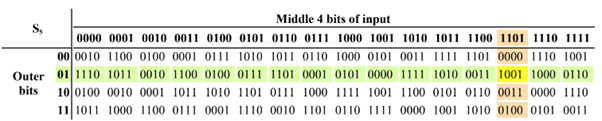
\includegraphics[width=\textwidth]{D:/trang/mật mã/báo cáo/Ảnh/hiền/s5.png}
    \caption{Ví dụ tra cứu $S_5$}
\end{figure}
Qua bước chuyển đổi với các hàm S-box, kết quả thu được là một giá trị 32 bit. Giá trị này sẽ được hoán vị lại theo hàm hoán vị $P$ để đưa ra kết quả cuối cùng của hàm $f$.
\begin{figure}[H]
	\includegraphics[scale=0.6]{"Ảnh/hiền/hoán vị P"}
	\caption{Bảng tra cứu hàm hoán vị $P$}
	\label{fig:hoan-vi-p}
\end{figure}
Giá trị 32 bit thu được từ các chuyển đổi với hàm lựa chọn S sẽ được đánh số từ 1 đến 32 theo thứ tự từ trái qua phải. Theo bảng hoán vị $P$, bit đầu tiên sau hoán vị sẽ là bit số 16, bit thứ 2 sẽ là bit số 7 và bit cuối cùng sẽ là bit số 25.Hàm tính toán mã hóa $f(R, K)$ được định nghĩa như sau:
\[\begin{gathered}
  f(R,K) = P({S_1}({B_1}){S_2}({B_2})...{S_8}({B_8})) \hfill \\
  {B_1}{B_2}...{B_8} = K \oplus E(R) \hfill \\ 
\end{gathered} \]
Trong đó: 
\begin{itemize}
    \item $P()$ là phép hoán vị $P$.
    \item $S_{n}$ là phép chuyển đổi block $n$ ($n$ chạy từ 1 đến 8 với hàm lựa chọn $S$).
    \item $B_{n}$ là block 6 bit thứ $n$ ($n$ chạy từ 1 đến 8). Block này lấy từ phép toán XOR giữa khóa vòng $K$ và giá trị hàm $E(R)$.
\end{itemize}
\subsubsection{Hàm phân phối Key (Key Schedule)}
Một key có 64 bit nhưng chỉ có 56 bit được sử dụng để thực hiện tính toán giá trị khóa vòng. Key được chia làm 8 byte. Các bit ở vị trí 8, 16, 32, 40, 48, 56 và 64 là các bit parity được sử dụng để kiểm tra độ chính xác của key theo từng byte vì khi key được phân phối trên đường truyền đến bộ mã hóa giải mã thì có thể xảy ra lỗi. Parity được sử dụng là parity lẻ (odd parity). Thuật toán tính khóa vòng được mô tả bởi hình dưới đây:
\begin{figure}[H]
	\centering
	\includegraphics[scale=0.7]{"Ảnh/hiền/khóa k"}
	\caption{Thuật toán tính khóa vòng}
	\label{fig:khoa-k}
\end{figure}
Key gốc sẽ được thực hiện hoán vị lựa chọn PC-1. Key được đánh số từ 1 đến 64 theo thứ tự từ trái qua phải.
\begin{figure}[H]
    \centering
    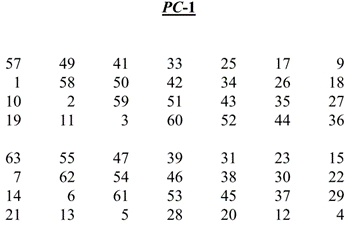
\includegraphics{Ảnh/hiền/pc-1.png}
    \caption{Bảng tra cứu PC-1}
\end{figure}
Bảng hoán vị lựa chọn PC-1 có hai phần. Phần đầu dùng để xác định giá trị $C_0$ và phần sau dùng để xác định giá trị $D_0$. Theo bảng trên thì $C_0$ là chuỗi bit có thứ tự là 57, 49, 41, ..., 36 lấy từ key gốc, $D_0$ là chuỗi bit có thứ tự là 63, 55, 47, ..., 4 lấy từ key gốc.\cite{Khanh2014}\\
\indent Sau khi xác định được giá trị ban đầu để tính key là $C_0$ và $D_0$ thì các khóa vòng $K_n$ (với $n$ từ 1 đến 16) sẽ được tính theo nguyên tắc giá trị của khóa vòng thứ $n$ sẽ được tính từ giá trị khóa vòng thứ $n-1$.
\[{K_n} = P{C_{ - 2}}({C_n}{D_n})\]
Trong đó: $C_{n}$ và $D_{n}$ được tạo từ $C_{n-1}$ và $D_{n-1}$ bằng cách dịch trái các giá trị này với số bit được quy định \cite{Khanh2014}.
\begin{figure}[H]
	\centering
	\includegraphics[scale=1]{"Ảnh/hiền/dịch trái"}
	\caption{Bảng quy định số bit dịch trái khi tính khóa vòng}
	\label{fig:dich-trai}
\end{figure}
Ví dụ, theo bảng trên, $C_{3}$ và $D_{3}$ có được từ $C_{2}$ và $D_{2}$ bằng cách dịch trái 2 bit. Hay $C_{16}$ và $D_{16}$ có được từ $C_{15}$ và $D_{15}$ bằng cách dịch trái 1 bit.
\begin{figure}[H]
	\centering
	\includegraphics[width=\textwidth]{"Ảnh/hiền/quy tắc dịch trái"}
	\caption{Minh họa phép dịch trái khi tính khóa vòng}
	\label{fig:quy-tac-dich-trai}
\end{figure}
Sau khi tính được $C_n$ và $D_n$ thì chuỗi $C_nD_n$ sẽ được đánh số từ 1 đến 56 theo thứ tự từ trái sang phải và được hoán vị lựa chọn lần 2 theo bảng hoán vị PC-2.
\begin{figure}[H]
    \centering
    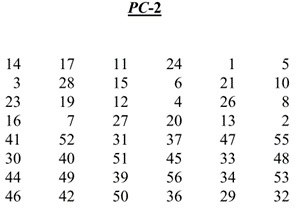
\includegraphics{D:/trang/mật mã/báo cáo/Ảnh/hiền/pc-2.png}
    \caption{Bảng tra cứu PC-2}
\end{figure}
Như vậy bit đầu tiên của khóa vòng $K_n$ là bit số 14 của chuỗi $C_nD_n$, bit thứ 2 là bit số 17 của chuỗi $C_nD_n$ và bit cuối cùng là bit số 32 của chuỗi $C_nD_n$.

\subsubsection{Hoán vị khởi tạo $IP^{-1}$}
Đây là bước cuối cùng để tạo ra giá trị mã hóa. Giá trị của lần lặp mã hóa cuối cùng sẽ được hoán vị khởi tạo đảo $IP^{-1}$ và tạo ra giá trị mã hóa plaintext.
\begin{figure}[H]
    \centering
    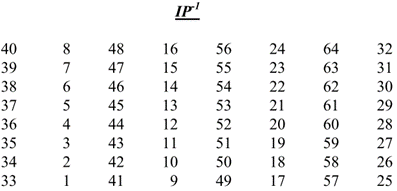
\includegraphics{D:/trang/mật mã/báo cáo/Ảnh/hiền/ip-1.png}
    \caption{Bảng tra cứu hoán vị đảo $IP^{-1}$}
\end{figure}
\subsubsection{Ví dụ về mã hóa DES}
Giả sử ta có dữ liệu cần mã hóa và key là: \\
M = 00123456789abcde (Hex) = 0000 0000 0001 0010 0011 0100 0101 0110 0111 1000 1001 1010 1011 1100 1101 1111. \\
K = 0133457799bbcdff (Hex) = 0000 0001 0011 0011 0100 0101 0111 0111 1001 10001 1011 1011 1100 1100 1111 1111.\\
Từ hai đầu vào này, giá trị của từng bước tính toán mã hóa DES sẽ được minh họa chi tiết sau đây.\cite{Khanh2014}
\begin{enumerate}
    \item Hoán vị khởi tạo - $IP$\\
    Thông điệp M được đánh số vị trí bit từ trái qua phải như sau:
    \begin{figure}[H]
        \centering
        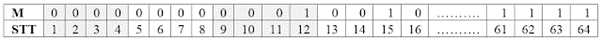
\includegraphics{D:/trang/mật mã/báo cáo/Ảnh/hiền/vs hoán vị.png}
        \caption{Hình ảnh minh họa thông điệp M}
    \end{figure}
    Sắp xếp lại thứ tự các bit của M theo bảng hoán vị $IP$, kết quả có được sau bước này là:
    $IP(M)$ = 98fecc00e054f0aa (Hex) = 1001 1000 1111 1110 1100 1100 0000 0000 1110 0000 0101 0100 1111 0000 1010 1010.
    \item Tính toán giá trị các khóa vòng – KS\\
    Để tính toán hàm mã hóa $f$, chúng ta cần có giá trị khóa cho từng lần lặp mã hóa. Key ban đầu được đánh số thứ tự bit từ trái qua phải.\\
    Sau khi sắp xếp các bit theo bảng hoán vị PC-1 ở trên, kết quả thu được là hai giá trị đầu như sau: 
    \begin{itemize}
        \item $C_{0}$ = f0ccaab (Hex) = 1111 0000 1100 1100 1010 1010 1011. 
        \item $D_{0}$ = aaccf0a (Hex) = 1010 1010 1100 1100 1111 0000 1010. 
    \end{itemize}
    Để tính khóa vòng đầu tiên $K_1$ thì $C_0$ và $D_0$ sẽ được dịch (quay) trái 1 bit. Giá trị thu được sau khi dịch trái là: 
    \begin{itemize}
        \item $C_{1}$ = e199557 (Hex) = 1110 0001 1001 1001 0101 0101 0111 
        \item $D_{1}$ = 5599e15 (Hex) = 0101 0101 1001 1001 1110 0001 0101 
    \end{itemize}
    Hai chuỗi $C_{1}$ và $D_{1}$ được ghép lài thành một chuỗi 56 bit là e1995575599e15. Chuỗi này được hoán vị bằng bảng PC-2 để được giá trị khóa vòng 48 bit thứ nhất $K_1$. 
    \begin{itemize}
        \item $K_1$ = 1b02efdb49a5 (Hex) 
    \end{itemize}
    Để tính khóa vòng $K_2$ thì lấy $C_{1}$ và $D_{1}$ dịch trái với số lượng bit theo bảng ở phần trên, rồi lấy kết quả hoán vị theo bảng PC-2. Quá trình cứ tiếp tục cho đến khóa vòng cuối cùng là $K_{16}$. Kết quả các khóa vòng 48 bit thu được là:
    \begin{itemize}
        \item $K_2$ = 69aed925ae66 (Hex) 
        \item $K_3$ = 55fc8ab4acd2 
        \item $K_4$ = 72add2ad8657 
        \item $K_5$ = 7cec071fe6c2 
        \item $K_6$ = 63a51e3cc545 
        \item $K_7$ = 6c84b78ae4c6 
        \item $K_8$ = f7883aece781 
        \item $K_9$ = c0dbeb27b839 
        \item $K_{10}$ = b1f347631d76 
        \item $K_{11}$ = 215fc30d89be 
        \item $_{K12}$ = 7171f5455cd5 
        \item $K_{13}$ = 95c5d14b80fd 
        \item $K_{14}$ = 5743b783đ8d 
        \item $K_{15}$ = bf91850a17b5 
        \item $K_{16}$ = cb3d0bbc7072
    \end{itemize}
    \item Tính hàm mã hóa $f(R,K)$
    Sau bước hoán vị khởi tạo $IP$, giá trị $IP(M)$ sẽ được tách làm hai phần là: 
    \begin{itemize}
        \item $R_{0}$ = e054f0aa (Hex) = 1110 0000 0101 0100 1111 0000 1010 1010. 
        \item $L_{0}$ = 98fecc00 (Hex) = 1001 1000 1111 1110 1100 1100 0000 0000. 
    \end{itemize}
    Giá trị 32 bit của $R_{0}$ được tra qua bảng E để tạo ra một giá trị 48 bit. 
    \begin{itemize}
        \item E($R_{0}$) = 7002a97a1555 (Hex). 
    \end{itemize}
    Giá trị này được XOR với khóa vòng thứ nhất K1 và được kết quả
    \begin{itemize}
        \item XOR(E($R_{0}$), $K_1$) = 6b0046a15cf0 (Hex).
    \end{itemize}
    Giá trị trên được chia thành 8 nhóm theo thứ tự từ trái qua phải, mỗi nhóm 6 bit để đưa đến các bảng $S$.
    \begin{figure}[H]
        \centering
        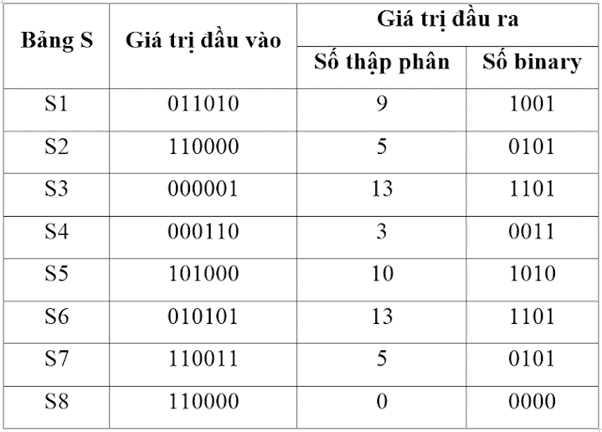
\includegraphics{D:/trang/mật mã/báo cáo/Ảnh/hiền/vd s-box.png}
        \caption{Bảng giá trị của biến đổi S-box}
    \end{figure}
    Các giá trị đầu ra sau bước tra các bảng $S$ sẽ được ghép lại theo thứ tự từ $S_1$ đến $S_8$ để được 1 giá trị 32 bit. 
    \begin{itemize}
        \item $S_1()S_2()S_3()S_4()S_5()S_6()S_7()S_8() = 10010101110100111010110101010000 = 95d3ad50$ (Hex). 
    \end{itemize}
    Giá trị này được hoán vị bằng bảng $P$ để cho ra giá trị của hàm $f$. 
    \begin{itemize}
        \item $f(R_{0},K_1)$ = 97d1619a (Hex) = 1001 0111 1101 0001 0110 0001 1001 1010. 
    \end{itemize}
    Tương tự, ta có giá trị hàm $f$ tại các vòng lặp mã hóa còn lại như sau: 
    \begin{itemize}
        \item $f(R_{1},K_2)$ = 88488d0b (Hex)
        \item $f(R_{2},K_3)$ = da3b2692 
        \item $f(R_{3},K_4)$ = f44950b2 
        \item $f(R_{4},K_5)$ = d83237fd 
        \item $f(R_{5},K_6)$ = afc43b25 
        \item $f(R_6,K_7)$ = 4e5123a2 
        \item $f(R_7,K_8)$ = 6cfdecb8 
        \item $f(R_8,K_9)$ = fb0600b1 
        \item $f(R_9,K_{10})$ = d51508e4 
        \item $f(R_{10},K_{11})$ = fcf67146 
        \item $f(R_{11},K_{12})$ = 704fa3a5 
        \item $f(R_{12},K_{13})$ = 7bfe2806 
        \item $f(R_{13},K_{14})$ = 65fc7a48 
        \item $f(R_{14},K_{15})$ = 513f1d11 
        \item $f(R_{15},K_{16})$ = cbf5252d
    \end{itemize}
    \item Giá trị tại mỗi vòng lặp mã hóa\\
    Giá trị của hàm $f(R,K)$ được sử dụng để tính giá trị $R_n$ và $L_n$ tại mỗi vòng lặp mã hóa theo công thức:
     \[\begin{gathered}
  {L_{n + 1}} = {R_n} \hfill \\
  {R_{n + 1}} = {L_n} \oplus f({R_n},{K_{n + 1}}) \hfill \\ 
\end{gathered} \]
    Thay vào công thức ở trên ta có các kết quả như sau:
    \begin{figure}[H]
        \centering
        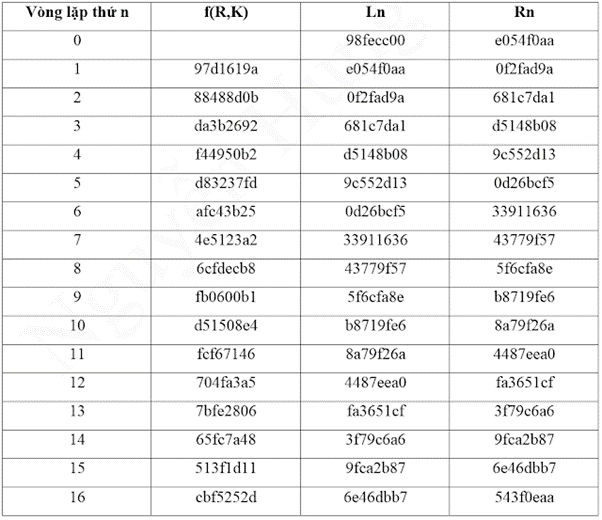
\includegraphics{D:/trang/mật mã/báo cáo/Ảnh/hiền/vs hàm f.png}
        \caption{Mô tả tính toán giá trị tại mỗi vòng lặp mã hóa}
    \end{figure}
    \item Hoán vị khởi tạp đảo $IP^-1$\\
    Giá trị $R_{16}$ và $L_{16}$ của vòng lặp mã hóa cuối cùng sẽ được ghép lại thành một chuỗi 64 bit để thực hiện hoán vị theo bảng $IP^{-1}$.\\
    Kết quả của phép hoán vị này chính là giá trị mã hóa (ciphertext) cần tính.\\
    $IP^{-1}(R_{16}, L_{16})$ = 1abff69d5a93e80b (Hex)\\
    = 0001 1010 1011 1111 1111 0110 1001 1101 0101 1010 1001 0011 1110 1000 0000 1011.

\end{enumerate}
\subsubsection{Thuật toán Giải mã Dữ liệu DES}
Các bước của quá trình giải mã dữ liệu được thực hiện tương tự như quá trình mã hóa dữ liệu. Trong quá trình giải mã có một số thay đổi như sau: 
Đầu vào lúc này là dữ liệu cần giải mã (Ciphertext) và đầu ra là kết quả giải mã được (Plaintext).\\
\indent Khóa vòng sử dụng trong các vòng lặp giải mã có thứ tự ngược với quá trình mã hóa. Nghĩa là, tại vòng lặp giải mã đầu tiên, khóa vòng được sử dụng là $K_{16}$. Tại vòng lặp giải mã thứ 2, khóa vòng được sử dụng là $K_{15}$, và tại vòng lặp giải mã cuối cùng thì khóa vòng được sử dụng là $K_1$ \cite{quan2020}.
\subsubsection{Nhận xét}
\begin{enumerate}
    \item Các thuộc tính của S-box:
    \begin{itemize}
    \item Các bit ra (output bit) luôn phụ thuộc không tuyến tính vào các bit vào (input bit) \cite{Khanh2014}.
    \item Sửa đổi ở một bit vào làm thay đổi ít nhất là hai bit ra \cite{Khanh2014}.
    \item Khi một bit vào được giữ cố định và 5 bit con lại cho thay đổi thì S-boxes thể hiện một tính chất được gọi là \textbf{“Phân bố Đồng nhất” (Uniform Distribution)}: so sánh số lượng bit số 0 và 1 ở các đầu ra luôn ở mức cân bằng. Tính chất này khiến cho việc áp dụng phân tích theo lý thuyết thông kê để tìm cách phá S-boxes là vô ích \cite{Khanh2014}.
    \end{itemize}
    => 3 tính chất này đảm bảo tốt tính chất \textbf{Nhập nhằng và Khuếch tán (Confusion \& Fiffusion)}.\\
    Thực tế, sau 8 vòng lặp tất cả các bit ra của DES sẽ chịu ảnh hưởng của tất cả các bit vào và tất cả các bit của khóa. Hơn nữa sự phụ thuộc này là rất phức tạp. Tuy nhiên sau này một số tấn công mới đã được đề xuất và cho thấy 8 vòng lặp này là chưa đủ để bảo mật \cite{Khanh2014}.
    \item Nhược điểm của thuật toán DES
    \begin{itemize}
    \item Điểm yếu chính trong DES là kích thước khóa, để thực hiện tấn công Brute Force, cần phải kiểm tra  $2^{56}$ khóa khả thi. Do đó, chúng ta nhận thấy:
    \begin{itemize}
        \item Với công nghệ hiện đại, có thể kiểm tra một triệu khóa mỗi giây, nghĩa là cần hơn hai nghìn năm để thực hiện Brute Force bằng máy tính với một bộ xử lý.
        \item Nếu có thể tạo ra máy tính với một triệu chip (xử lý song song), thì có thể kiểm tra toàn bộ không gian khóa trong 20 giờ. Vào năm 1998, máy tính đã có thể tìm thấy khóa DES trong 112 giờ.
        \item Mạng máy tính có thể mô phỏng xử lý song song bằng cách chia không gian khóa giữa nhiều máy tính để thực hiện tấn công Brute Force. Có thể giả định rằng mạng với 42.000 thành viên có thể tìm thấy khóa trong 10 ngày.
        \item Tốc độ của các triển khai phần cứng: Mặc dù các triển khai DES trên phần cứng có thể rất nhanh, nhưng điều này không hẳn là một lợi thế về mặt bảo mật. Nếu phần cứng có thể thực hiện một lượng lớn phép mã hóa và giải mã trong thời gian ngắn, thì thời gian cần thiết để thử tất cả các khóa có thể cũng giảm xuống đáng kể.
        \item Hiệu suất chậm trên phần mềm: DES không được thiết kế ban đầu để chạy trên phần mềm, dẫn đến hiệu suất chậm khi thực thi trên các máy tính thông thường. 
    \end{itemize}
\end{itemize}
\end{enumerate}
\subsubsection{ Mặt hạn chế của DES}
\begin{itemize}
    \item Tốc độ của các triển khai phần cứng: Mặc dù các triển khai DES trên phần cứng có thể rất nhanh, nhưng điều này không hẳn là một lợi thế về mặt bảo mật. Nếu phần cứng có thể thực hiện một lượng lớn phép mã hóa và giải mã trong thời gian ngắn, thì thời gian cần thiết để thử tất cả các khóa có thể cũng giảm xuống đáng kể.
    \item Hiệu suất chậm trên phần mềm: DES không được thiết kế ban đầu để chạy trên phần mềm, dẫn đến hiệu suất chậm khi thực thi trên các máy tính thông thường. 
    \item Điểm yếu chính trong DES là kích thước khóa, để thực hiện tấn công brute force, cần phải kiểm tra $2^{56}$ khóa khả thi \cite{Wikipedia}. Do đó, chúng ta nhận thấy:
 \begin{itemize}
     \item Với công nghệ hiện đại, có thể kiểm tra một triệu khóa mỗi giây, nghĩa là cần hơn hai nghìn năm để thực hiện Brute Force bằng máy tính với một bộ xử lý.
    \item Nếu có thể tạo ra máy tính với một triệu chip (xử lý song song), thì có thể kiểm tra toàn bộ không gian khóa trong 20 giờ. Vào năm 1998, máy tính đã có thể tìm thấy khóa DES trong 112 giờ.
   \item Mạng máy tính có thể mô phỏng xử lý song song bằng cách chia không gian khóa giữa nhiều máy tính để thực hiện tấn công Brute Force. Có thể giả định rằng mạng với 42.000 thành viên có thể tìm thấy khóa trong 10 ngày.

\end{itemize}
    
\end{itemize}
\subsection{Thuật toán AES}
Vào năm 2000, Cơ quan quản lý về chuẩn và công nghệ của Mỹ, NIST (National Institute of Standard and Technology), đã tổ chức một cuộc thi để chọn một hệ mật mã mới thay thế cho DES. Hệ mã Rijndael đã đựợc chọn và được công bố (2002) như là chuẩn mật mã mới thay thế cho DES, với tên gọi là Advanced Encryption Standard (AES). Vào đến vòng trong còn có các ứng viên khác là RC6, Serpent, MARS và Twofish. Hệ mã này được phát triển bởi 2 nhà khoa học Bỉ, Joan Daemen và Vincent Rijnmen (vì vậy tên gọi Rijndael được tạo ra từ việc ghép tiền tố tên họ 2 ông này).\\
\indent AES được xây dựng trên nguyên lý thiết kế lưới giao hoán – thay thế (Substitution-Permutation Network). Đây là một hệ mã có tốc độ tốt trong cả cài đặt phần mềm cũng như phần cứng. Khác với DES, AES không theo mẫu thiết kế mạng Feistel. Thay vào đó các thao tác cơ bản được thực hiện trên các khối ma trận dữ liệu 4 $\times 4$ (bytes), được gọi là các trạng thái (state). Số vòng lặp của AES là một tham số xác định trên cơ sở kích thước khóa: 10 vòng lặp cho khóa 128 bit, 12 vòng cho 192 bit, 14 vòng cho 256 bit. Trong bài báo cáo này chúng em sẽ tìm hiểu sâu hơn về ASE-128.

\subsubsection{Quá trình mã hóa của Thuật toán AES-128}
Mã hóa AES được thực hiện thông qua 5 chức năng chính là AddRoundKey, SubBytes, ShiftRows, MixColumns và KeyExpansion. Năm chức năng này được sắp xếp để thực hiện ba bước cơ bản.
\begin{itemize}
    \item \textbf{Bước 1}: Bước khởi tạo: dữ liệu cần được mã hóa plain\_text[127:0] kết hợp với key[127:0] bằng chức năng AddRoundKey.
    \item \textbf{Bước 2}: Bước lặp mã hóa: kết quả bước 1 được sử dụng để thực hiện tuần tự các chức năng SubBytes, ShiftRows, MixColumns và AddRoundKey. Bước này được lặp lại 9 lần. Chú ý, KeyExpansion thực hiện song song với bước AddRoundKey để tạo khóa vòng cho chức năng này.
    \item \textbf{Bước 3}: Bước tạo ngõ ra: Sau 9 lần lặp ở bước 2, kết quả được sử dụng để thực hiện tuần tự các chức năng SubBytes, ShiftRows và AddRoundKey để tạo ngõ ra cipher\_text[127:0].
\end{itemize}
\begin{figure}[H]
    \centering
    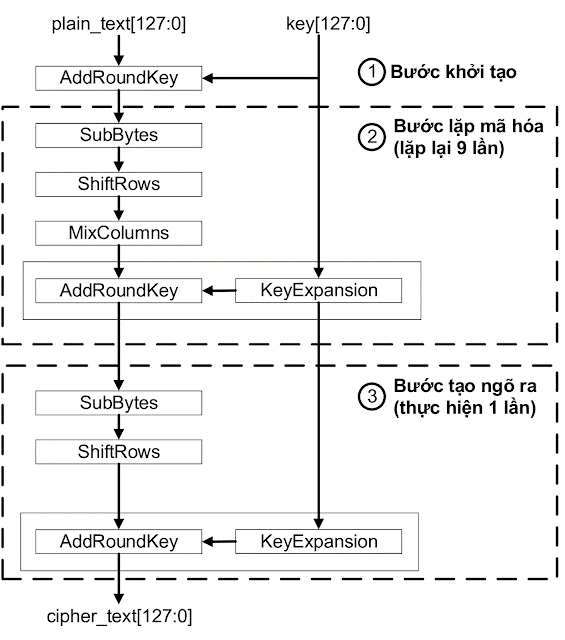
\includegraphics[width=\textwidth]{Ảnh/hiền/mã hóa aes.png}
    \caption{Quá trình mã hóa AES-128}
\end{figure}
Tất cả các phép toán được tổ hợp dựa vào phép tính XOR và các bảng dữ liệu nên rất nhanh và hiệu quả. Thuật toán cũng hiệu quả hơn cho các máy tính 32 bit.\\
VD: Giả sử chuỗi dữ liệu cần mã hóa plain\_text[127:0] và khóa mã key[127:0] có giá trị như sau:
\begin{itemize}
    \item plain\_text[127:0] = 32 43 f6 a8 88 5a 30 8d 31 31 98 a2 e0 37 07 34
    \item key[127:0] = 2b 7e 15 16 28 ae d2 a6 ab f7 15 88 09 cf 4f 3c
\end{itemize}
Dữ liệu và khóa mã được sắp xếp dưới dạng ma trận với mỗi phần tử là một byte.
\begin{figure}[H]
    \centering
    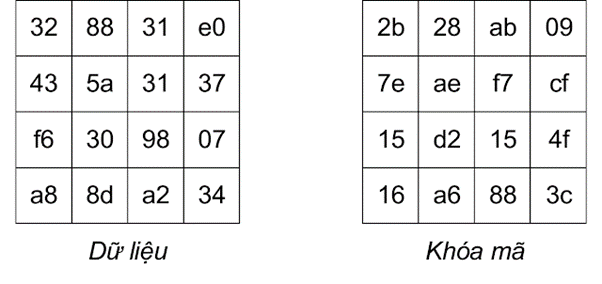
\includegraphics{Ảnh/hiền/vd aes.png}
    \caption{Dữ liệu và khóa mã được sắp xếp dưới dạng ma trận}
\end{figure}
Trong quá trình mã hóa, ma trận dữ liệu ban đầu sẽ bị biến đổi bởi các chức năng AddRoundKey, SubBytes, ShiftRows hoặc MixColumns để tạo ra các dữ liệu trung gian gọi là ma trận trạng thái. Ma trận khóa mã sẽ bị biến đổi bởi chức năng KeyExpansion để tạo ra các khóa mã trung gian gọi là khóa vòng.
\begin{itemize}
    \item \textbf{Chức năng AddRoundKey}: Chức năng AddRoundKey thực hiện ở:
    \begin{enumerate}
        \item Bước khởi tạo: $XOR$ khóa mã với ma trận dữ liệu
        \item Bước lặp mã hóa và bước tạo ngõ ra: $XOR$ khóa vòng (round key) với ma trận trạng thái. 
        \begin{figure}[H]
            \centering
            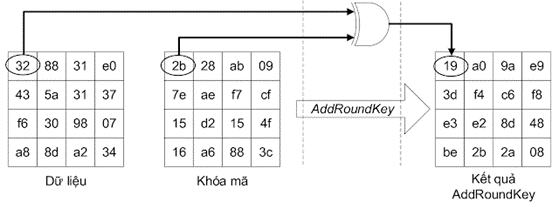
\includegraphics{Ảnh/hiền/addround.png}
            \caption{Chức năng AddRoundKey cho bước khởi tạo}
        \end{figure}
        Đối với bước lặp mã hóa và bước tạo ngõ ra, vị trí "khóa mã" là các "khóa vòng" còn dữ liệu là của lần tính trước đó.
    \end{enumerate}
    \item \textbf{Chức năng SubBytes}: Chức năng SubBytes là thực hiện thay thế từng byte của ma trận trạng thái, ngõ ra của AddRoundKey, bằng một giá trị đã quy định trong chuẩn AES. Bảng quy định giá trị thay thế gọi là S-box.
    \begin{figure}[H]
        \centering
        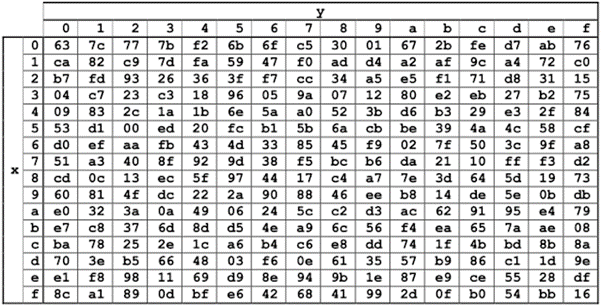
\includegraphics{Ảnh/hiền/s-box aes.png}
        \caption{S-box của mã hóa AES}
    \end{figure}
    Ví dụ, byte cần thay thế là H08 thì dò ở hàng số 0 và cột số 8 trong bảng S-box sẽ được kết quả là 30.
    \begin{figure}[H]
        \centering
        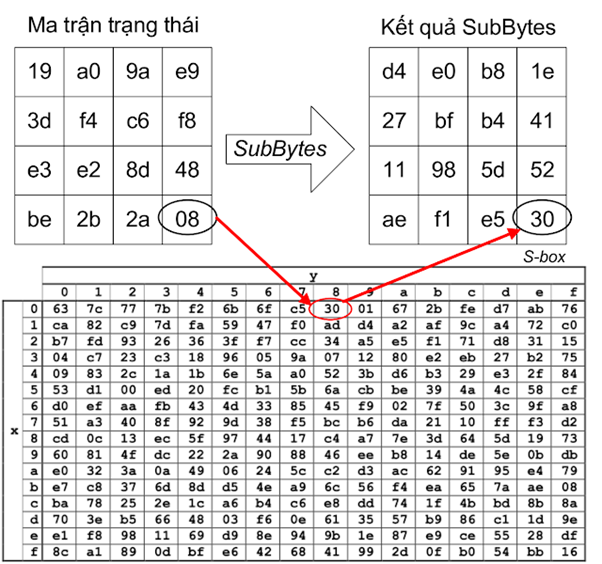
\includegraphics{Ảnh/hiền/vd h08.png}
        \caption{Mô tả kết quả biến đổi của H08}
    \end{figure}
    \item \textbf{Chức năng ShiftRows}: Chức năng ShiftRows thực hiện quay trái từng hàng của ma trận trạng thái, ngõ ra của SubBytes, theo byte với hệ số quay tăng dần từ 0 đến 3. Hàng đầu tiên có hệ số quay là 0 thì các byte được giữ nguyên vị trí. Hàng thứ hai có hệ số quay là 1 thì các byte được quay một byte. Hàng thứ ba quay hai byte và hàng thứ tư quay ba byte.
    \begin{figure}[H]
        \centering
        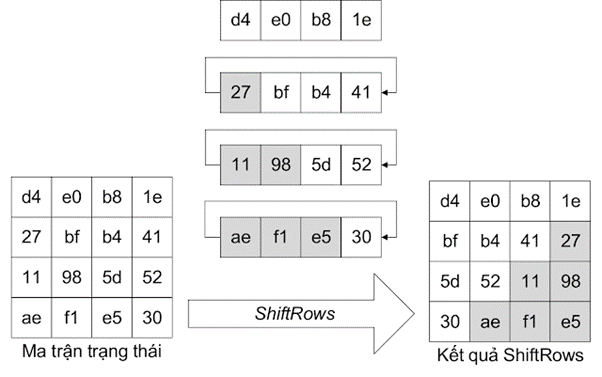
\includegraphics{Ảnh/hiền/shiftrow vd.png}
        \caption{Mô tả chức năng ShiftRows}
    \end{figure}
    \item \textbf{Chức năng MixColumns}: Chức năng MixColumns thực hiện nhân từng cột của ma trận trạng thái, ngõ ra của ShiftRows, với một ma trận chuyển đổi quy định bởi chuẩn AES.
    \begin{figure}[H]
        \centering
        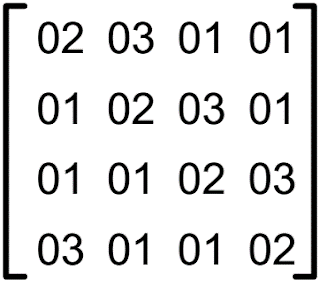
\includegraphics{Ảnh/hiền/mix.png}
        \caption{Ma trận chuyển đổi sử dụng trong chức năng MixColumns}
    \end{figure}
    Việc biến đổi một cột của ma trận trạng thái được thực hiện bởi hai phép toán là nhân và $XOR$.\\
    VD: Biểu thức sau tạo ra phần tử H04, H là ký hiệu của số Hex, ở cột 1 trong hình minh họa "chức năng MixColumns".\\
    $H04 =Hd4.H02 + Hbf.H03 + H5d.H01 + H30.H01=Hd4.H02 + (Hbf.H02 + Hbf.H01) + H5d.H01 + H30.H01$ 
    \begin{figure}[H]
        \centering
        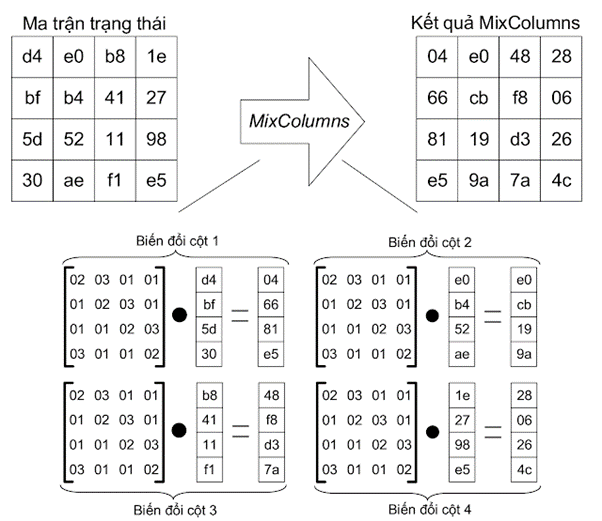
\includegraphics{Ảnh/hiền/vd mix.png}
        \caption{Mô tả chức năng MixColoumns}
    \end{figure}
    Phép nhân với H01 thì giữ nguyên giá trị. Phép nhân với H02 tương đương với việc dịch trái một bit và XOR có điều kiện như sau:
    \begin{itemize}
        \item Nếu bit MSB của giá trị được dịch bằng 1 thì giá trị sau khi dịch được $XOR$ với H1b.
        \item Nếu bit MSB của giá trị được dịch bằng 0 thì giữ giá trị sau khi dịch.
    \end{itemize}
    \begin{figure}[H]
        \centering
        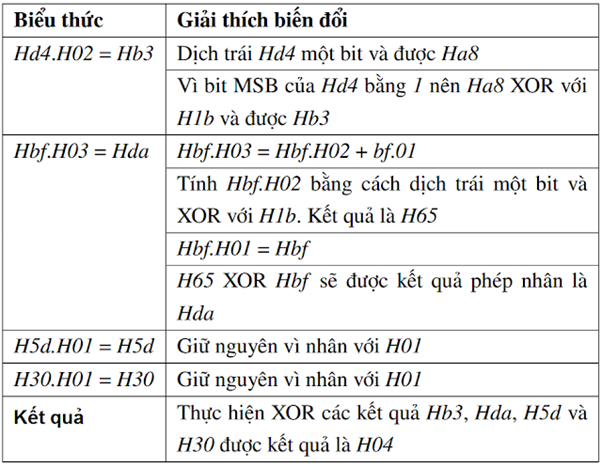
\includegraphics{Ảnh/hiền/mix h04.png}
        \caption{Chi tiết về cách tính MixColoums tạo ra phần từ H04 ở cột 1}
    \end{figure}
    \item \textbf{Chức năng KeyExpansion}: \\
    Chức năng KeyExpansion thực hiện tính toán khóa vòng cho bước lặp mã hóa và bước tạo ngõ ra. Kết quả của một lần thực thi KeyExpansion là một khóa vòng sử dụng cho chức năng AddRoundKey. Với mã hóa AES-128, số khóa vòng là 10 tương ứng với 9 lần AddRoundKey ở bước lặp mã hóa và 1 lần AddRoundKey ở bước tạo ngõ ra.\\
    Chức năng KeyExpansion được thực hiện thông qua 4 chức năng là RotWord, SubWord, AddRcon và AddW.
    \begin{figure}[H]
        \centering
        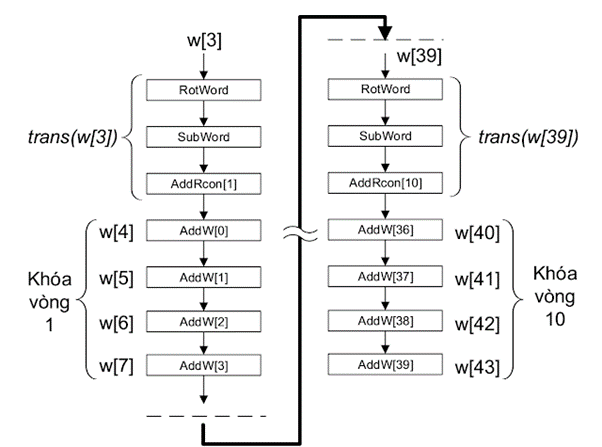
\includegraphics{Ảnh/hiền/keyexpan.png}
        \caption{Chức năng KeyExpansion}
        
    \end{figure}
    Mỗi khóa vòng có 128 bit được chia làm 4 word, mỗi word là 4 byte và ký hiệu là w[j] với j là số nguyên. Mã hóa AES-128 có 1 khóa mã và 10 khóa vòng nên tổng số từ là 44 và được đánh số từ 0 đến 43. Khóa mã có 4 từ là w[0], w[1], w[2] và w[3]. Khóa vòng 1 có 4 từ là w[4], w[5], w[6] và w[7]. Tương tự, khóa vòng 10 có 4 từ là w[40], w[41], w[42] và w[43].\\
    Từ w[j] tính theo công thức sau, với 3 < j < 44.\\
    $w[j] = AddW[j - 4] = w[j - 1] + w[j - 4]$ \\  
    $w[j = 4*n] = AddW[j - 4] = trans(w[j - 1])+ w[j - 4]$\\
    Chú ý, khi tính các từ ở vị trí j là bội số của 4, như w[4], w[8],... và w[40], thì w[j-1] phải được biến đổi qua 3 chức năng RotWord, SubWord và AddRcon, gọi là trans(w[j-1]), trước khi XOR với w[j-4].\\
    Khóa mã key ở mục 1 được sử dụng để minh họa việc tính toán khóa vòng. Khóa mã key[127:0] được chia làm 4 từ như biểu thức sau:\\
    $w[0] = 2b7e1516 w[1] = 28aed2a6$ \\
    $w[2] = abf71588 w[3] = 09cf4f3c$\\
    Việc tính toán khóa vòng 1 là thực hiện tính 4 từ w[4], w[5], w[6] và w[7]. Để tính khóa vòng 1, trans(w[3]) phải được tính trước thông qua 3 chức năng RotWord, SubWord và AddRcon.\\
    $w[4] = AddW[0] = trans(w[3])+ w[0]w[5] = AddW[1] = w[4]+ w[1]w[6] = AddW[2] = w[5]+ w[2]w[7] = AddW[3] = w[6]+ w[3]$\\
    Chức năng RotWord Chức năng RotWord thực hiện quay trái từ w[j] một byte.
    \begin{figure}[H]
        \centering
        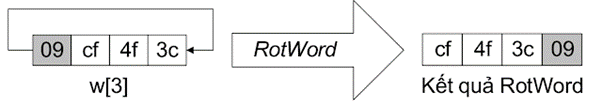
\includegraphics{Ảnh/hiền/rword.png}
        \caption{Thực thi RotWord cho từ w[3]}
    \end{figure}
    Chức năng SubWord thực hiện thay thế các phi tuyến từng byte của kết quả RotWord theo bảng S-box.
    \begin{figure}[H]
        \centering
        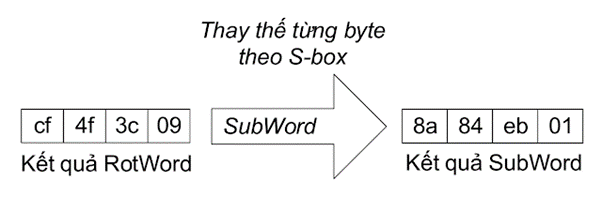
\includegraphics{Ảnh/hiền/subw.png}
        \caption{Thực thi SubWord khi chuyển đổi từ w[3]}
    \end{figure}
    Chức năng AddRcon thực hiện XOR kết quả SubWord và giá trị Rcon[j/4] với j là bội số của 4. Số lượng giá trị Rcon[j/4] là 10 tương ứng với 10 lần tính khóa vòng. Chức năng AddRcon sẽ tạo ra kết quả cuối cùng của biến đổi trans(w[j-1]).
    \begin{tabular}{|c|c|c|}
    
\hline
\textbf{Rcon[j/4]} & \textbf{Giá trị HEX} & \textbf{Vị trí sử dụng} \\
\hline
Rcon[1] & 01000000 & sử dụng cho trans(w[3]) khi tính w[4] \\
Rcon[2] & 02000000 & sử dụng cho trans(w[7]) khi tính w[8] \\
Rcon[3] & 04000000 & sử dụng cho trans(w[11]) khi tính w[12] \\
Rcon[4] & 08000000 & sử dụng cho trans(w[15]) khi tính w[16] \\
Rcon[5] & 10000000 & sử dụng cho trans(w[19]) khi tính w[20] \\
Rcon[6] & 20000000 & sử dụng cho trans(w[23]) khi tính w[24] \\
Rcon[7] & 40000000 & sử dụng cho trans(w[27]) khi tính w[28] \\
Rcon[8] & 82000000 & sử dụng cho trans(w[31]) khi tính w[32] \\
Rcon[9] & 1b000000 & sử dụng cho trans(w[35]) khi tính w[36] \\
Rcon[10] & 36000000 & sử dụng cho trans(w[39]) khi tính w[40] \\
\hline
\end{tabular}
\begin{figure}[H]
    \centering
    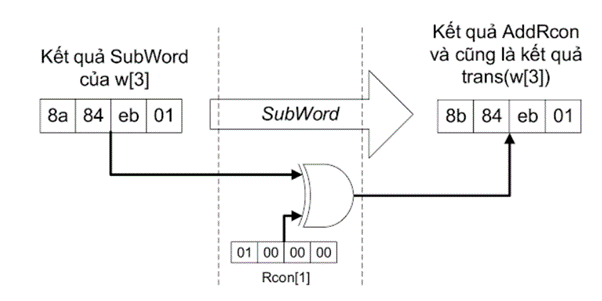
\includegraphics{Ảnh/hiền/addcon.png}
    \caption{Thực thi AddRcon khi chuyển đổi từ w[3]}
\end{figure}
Chức năng AddW thực hiện XOR w[j-4] với w[j-1] hoặc trans(w[j-1]) như công thức 4.8 để tạo ra khóa vòng.
\begin{figure}[H]
    \centering
    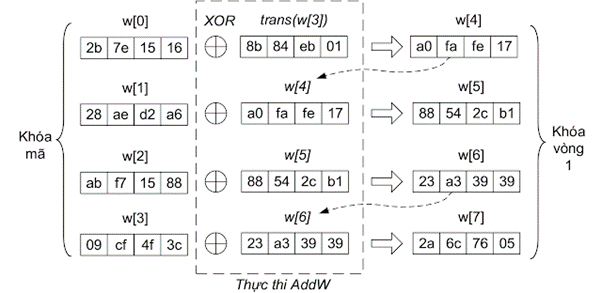
\includegraphics{Ảnh/hiền/addw.png}
    \caption{Thực thi AddW}
\end{figure}
\end{itemize}
\subsubsection{Quá trình giải mã của Thuật toán AES-128}

Mã hóa chuyển một "bản rõ" (Plaintext) thành một "bản mã" (Ciphertext) thông qua một khóa mã (key) giúp che dấu thông tin gốc ban đầu. Giải mã là quá trình nghịch đảo (Inverse Cipher) của quá trình mã hóa. Nó giúp khôi phục lại bản rõ từ một bản mã \cite{abdullah2017advanced}.

Thuật toán giải mã khá giống với thuật toán mã hóa về mặt cấu trúc nhưng 4 hàm sử dụng là 4 hàm ngược của quá trình mã hóa.
\begin{figure}[H]
    \centering
    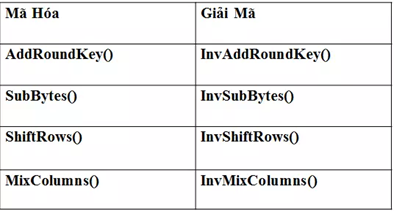
\includegraphics[scale=1]{pic/huê/ngc mã hóa.png}
    
    
    \caption{Các chức năng ngược nhau trong mã hóa và giải mã AES}
\end{figure}

Các bước giải mã:
\begin{itemize}
    \item Bước 1. Bước khởi tạo: Dữ liệu cần được mã hóa cipher\_text[127:0] kết hợp với khóa vòng thứ 10, round\_key\_10[127:0], bằng chức năng AddRoundKey.
    \item Bước 2. Bước lặp giải mã: kết quả bước 1 được sử dụng để thực hiện tuần tự các chức năng InvShiftRows, InvSubBytes, AddRoundKey và InvMixColumns. Bước này được lặp lại 9 lần.
    \item Bước 3. Bước tạo ngõ ra: Sau 9 lần lặp ở bước 2, kết quả được sử dụng để thực hiện tuần tự các chức năng InvShiftRows, InvSubBytes và AddRoundKey với khóa mã ban đầu để khôi phục lại plain\_text[127:0].
\end{itemize}

So sánh giữa quá trình mã hóa và giải mã như sau:

\begin{figure}[H]
    \centering
    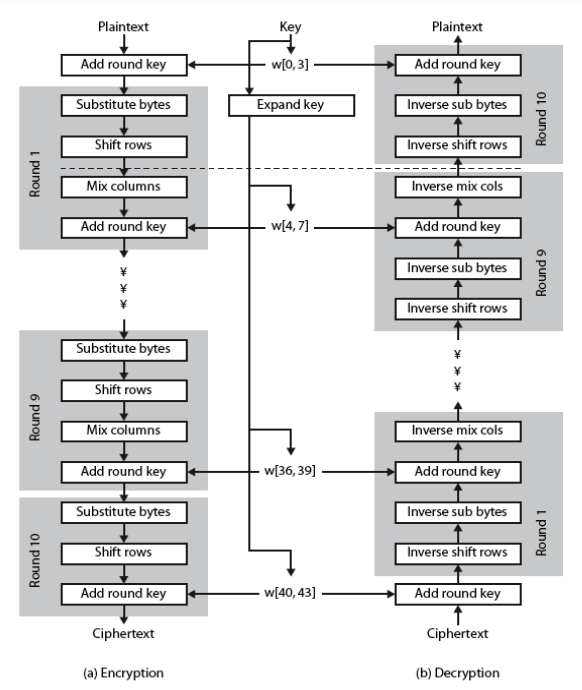
\includegraphics[scale=1.4]{pic/huê/AES mã hóa và giải mã.png}
    
    
    \caption{Quá trình mã hóa và giải mã AES}
\end{figure}

Quá trình giải mã AES-128 sẽ được giải thích trên một ví dụ cụ thể. Giả sử chuỗi dữ liệu cần mã hóa cipher\_text[127:0] và khóa vòng cuối cùng lấy từ quá trình mã hóa key[127:0] có giá trị như sau:
\begin{itemize}
    \item cipher\_text[127:0] =  69 c4 e0 d8 6a 7b 04 30 d8 cd b7 80 70 b4 c5 5a.
    \item key[127:0] = 13 11 1d 7f e3 94 4a 17 f3 07 a7 8b 4d 2b 30 c5.
\end{itemize}

Dữ liệu và khóa mã được sắp xếp dưới dạng ma trận với mỗi phần tử là một byte.
\begin{figure}[H]
    \centering
    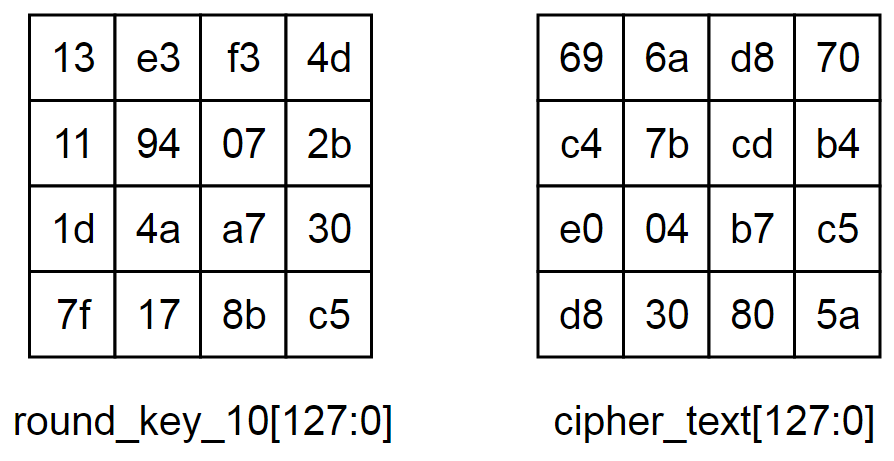
\includegraphics[scale=0.4]{pic/huê/input giải mã.png}
    
    
    \caption{Ma trận khóa vòng thứ 10 và ma trận dữ liệu đã mã hóa}
\end{figure}

\begin{itemize}
    \item Chức năng InvAddRoundKey:

    Chức năng InvAddRoundKey trong quá trình giải mã cũng chính là chức năng AddRoundKey trong quá trình mã hóa nên gọi chung là AddRoundKey.\cite{b3}

    \begin{figure}[H]
    \centering
    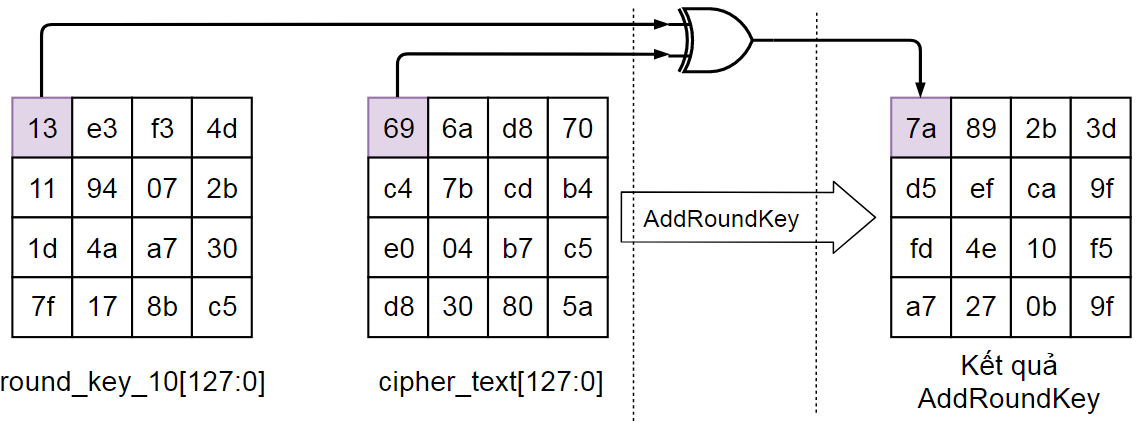
\includegraphics[scale=0.4]{pic/huê/Chức năng AddRoundKey đảo.png}
    
    
    \caption{Chức năng InvAddRoundKey}
\end{figure}
\item Chức năng InvShiftRows:
InvShiftRows là đảo của chức năng ShiftRows. InvShiftRows thực hiện quay phải từng hàng của ma trận trạng thái, sinh ra từ bước trước đó, theo byte với hệ số quay tăng dần từ 0 đến 3. Hàng đầu tiên có hệ số quay là 0 thì các byte được giữ nguyên vị trí. Hàng thứ hai có hệ số quay là 1 thì các được quay một byte. Hàng thứ ba quay hai byte và hàng thứ tư quay ba byte \cite{fips2001197}.
\begin{figure}[H]
    \centering
    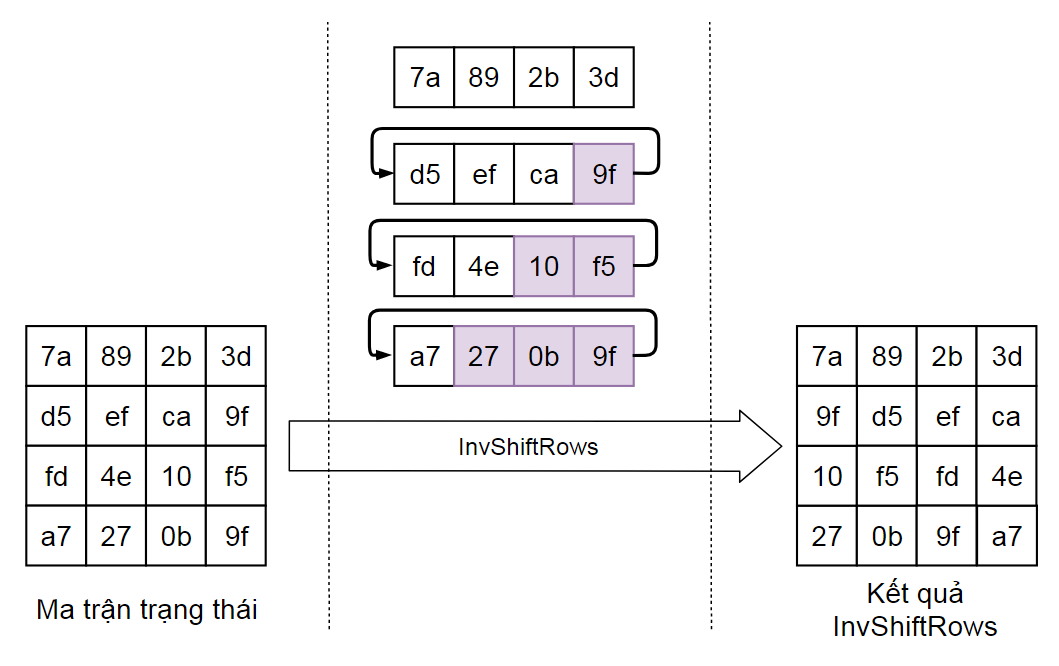
\includegraphics[scale=0.4]{pic/huê/Chức năng InvShiftRows.png}
    
    
    \caption{Chức năng InvShiftRows}
\end{figure}
\item Chức năng InvSubBytes:
Chức năng InvSubBytes là thực hiện thay thế từng byte của ma trận trạng thái, bằng một giá trị đã quy định trong chuẩn AES. Bảng quy định giá trị thay thế cho InvSubBytes gọi là S-box đảo (Inverse S-box) \cite{fips2001197}.
\begin{figure}[H]
    \centering
    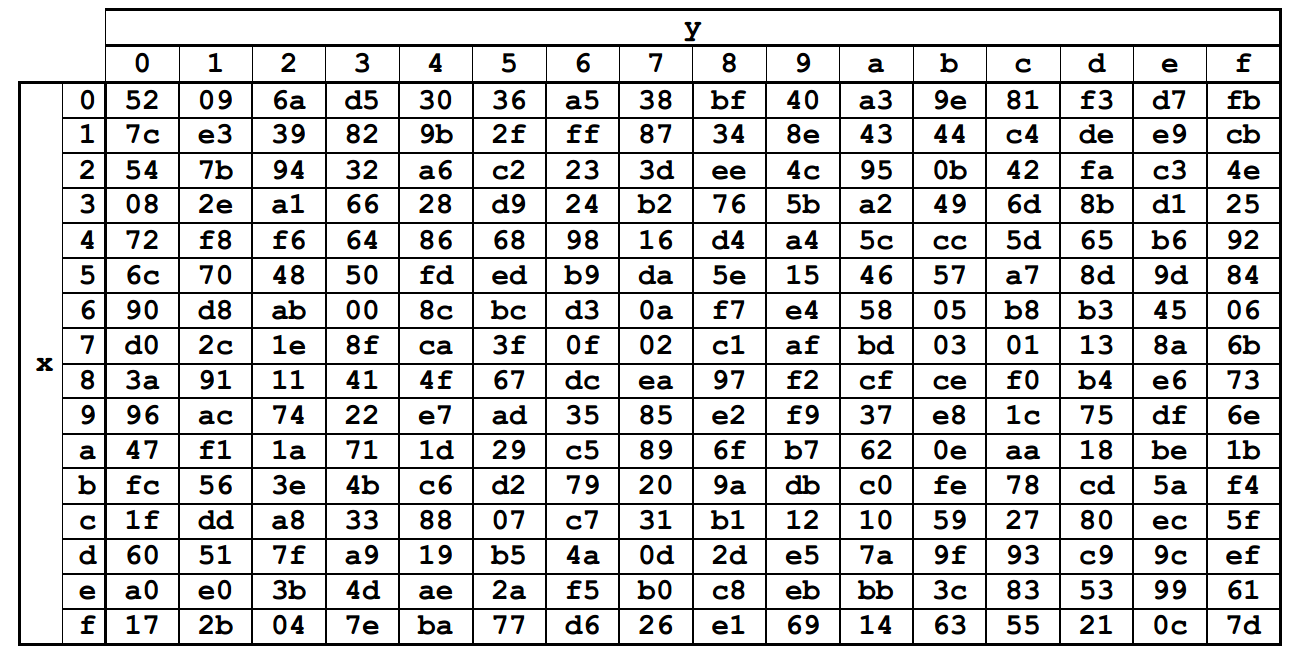
\includegraphics[scale=0.3]{pic/huê/bảng S-box Inv.png}
    
    \caption{Bảng S-box đảo của chuẩn AES}
\end{figure}
Ví dụ, byte cần thay thế là Ha7 thì dò ở hàng "a" và cột số 7 trong bảng S-box đảo sẽ được kết quả là H89.
\begin{figure}[H]
    \centering
    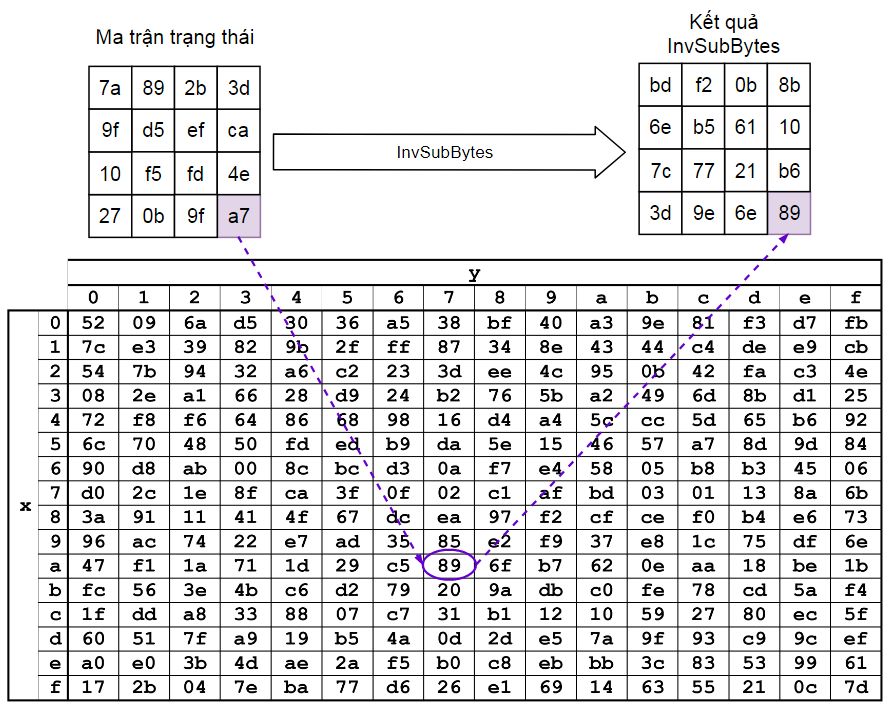
\includegraphics[scale=0.5]{pic/huê/Chức năng InvSubBytes.png}
    
    \caption{Chức năng InvSubBytes}
\end{figure}
\item Chức năng InvMixColumns:

InvMixColumns của quá trình giả mã là đảo của MixColumns trong quá trình mã hóa. Từng cột của ma trận trạng thái sẽ được nhân với ma trận chuyển đổi sau đây.\cite{fips2001197}

\begin{figure}[H]
    \centering
    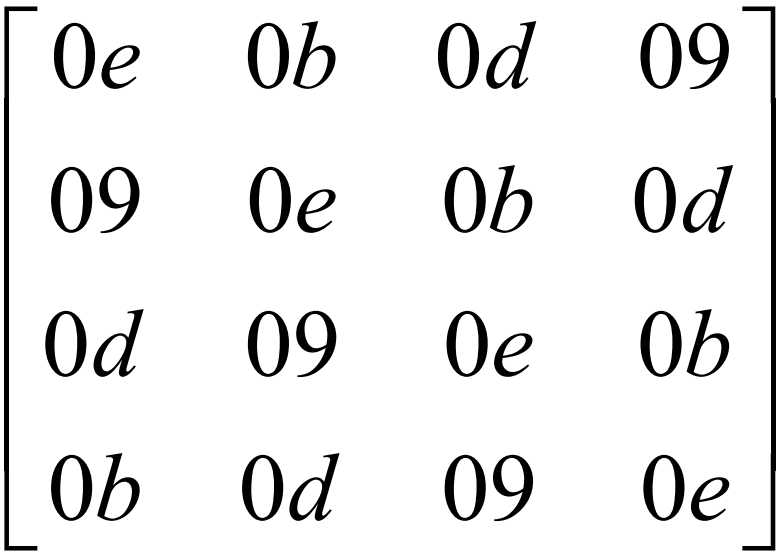
\includegraphics[scale=0.2]{pic/huê/Ma trận chuyển đổi dùng trong InvMixColumns.png}
    
    \caption{Ma trận chuyển đổi dùng trong InvMixColumns}
\end{figure}

Cách tính InvMixColumns sẽ được trình bày sau đây: \\

\textbf{Phép nhân một byte A với H0e:}
\begin{center}
    $A.H0e = A.H08 + A.H04 + A.H02$
\end{center}

    Trong đó, phép nhân với H04 và H08 hoàn toàn có thể chuyển về phép nhân với H02:
\begin{center}
    $A.H04 = A.H02.H02$
    
$A.H08 = A.H02.H02.H02 $
\end{center}
    
Suy ra: 
\begin{center}
    $A.H0e = A.H02.H02.H02 + A.H02.H02 + A.H02 $
\end{center}

\textbf{Phép nhân một byte A với H0b:}
\begin{center}
    $A.H0b = A.H08 + A.H02 + A.H01 = A.H02.H02.H02 + A.H02 + A.H01 $
\end{center}

\textbf{Phép nhân một byte A với H0d:}
\begin{center}
    $A.H0d = A.H08 + A.H04 + A.H01 = A.H02.H02.H02 + A.H02.H02 + A.H01 $
\end{center}

\textbf{Phép nhân một byte A với H09:}
\begin{center}
    $A.H0e = A.H08 + A.H01 = A.H02.H02.H02 + A.H01$
\end{center}

Việc tính InvMixColumn cho toàn bộ một ma trận trạng thái như sau:

\begin{figure}[H]
    \centering
    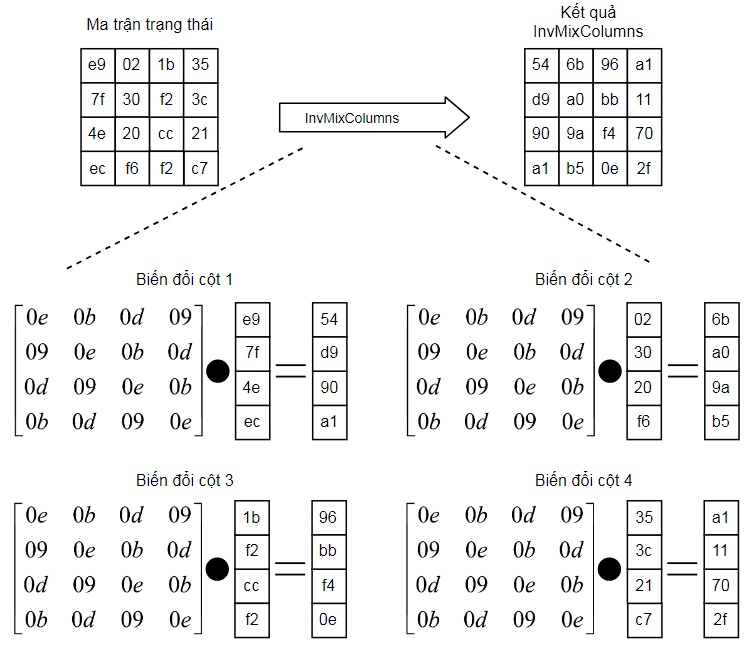
\includegraphics[scale=0.5]{pic/huê/Chức năng InvMixColumns.png}
    
    \caption{Chức năng InvMixColumns}
\end{figure}

Với việc quy đổi phép nhân về dạng nhân với H02 và H01. Mạch logic nhân một byte với H0e, H0b, H0d và H09 có thể được thực hiện như hình sau.

\begin{figure}[H]
    \centering
    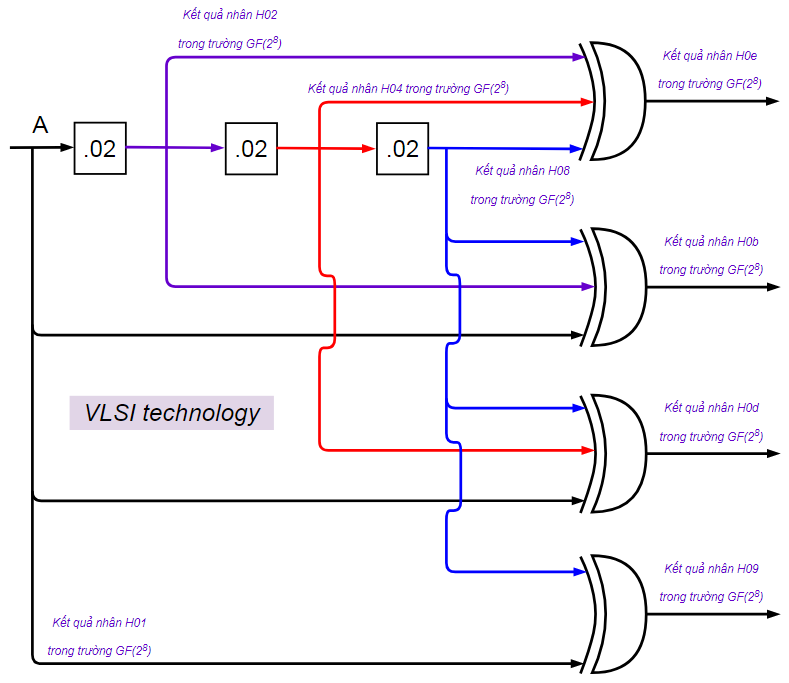
\includegraphics[scale=0.5]{pic/huê/Mạch nguyên lý nhân một byte A với các phần tử trong ma trận chuyển đổi InvMixColumns.png}
    
    \caption{Mạch nguyên lý nhân một byte A với các phần tử trong ma trận chuyển đổi InvMixColumns}
\end{figure}
\end{itemize}

\subsubsection{Các dạng tấn công vào AES}
\begin{itemize}
    \item Side-channel Attack:
    \begin{itemize}
        \item Side Channels (Kênh kề) được định nghĩa là các kênh đầu ra không mong muốn từ một hệ thống.
        \item Tấn công kênh bên hay còn gọi là Tấn công kênh kề là loại tấn công dễ thực hiện trong các loại tấn công mạnh chống lại quá trình triển khai mã hóa, và mục tiêu của loại tấn công này là phân tích các nguyên tố, các giao thức, module, và các thiết bị trong mỗi hệ thống.
        \item Một số loại tấn công kênh kề như: Tấn công thời gian, tấn công dựa vào lỗi, tấn công phân tích năng lượng, tấn công phân tích điện từ
        \item Tấn công kênh bên hay còn gọi là Tấn công kênh kề là loại tấn công dễ thực hiện trong các loại tấn công mạnh chống lại quá trình triển khai mã hóa, và mục tiêu của loại tấn công này là phân tích các nguyên tố, các giao thức, module, và các thiết bị trong mỗi hệ thống.
        \item Một số loại tấn công kênh kề như: Tấn công thời gian, tấn công dựa vào lỗi, tấn công phân tích năng lượng, tấn công phân tích điện từ.
    \end{itemize}

    \item Known Attacks:
    \begin{itemize}
        \item Vào năm 2002, Nicolas Courtois và Josef Pieprzyk phát hiện một tấn công trên lý thuyết gọi là tấn công XSL và chỉ ra điểm yếu tiềm tàng của AES.
        \item Tuy nhiên, một vài chuyên gia về mật mã học khác cũng chỉ ra một số vấn đề trong Cơ sở Toán học của tấn công này và cho rằng các tác giả đã có sai lầm trong tính toán. Việc tấn công dạng này có thực sự trở thành hiện thực hay không vẫn còn để ngỏ và cho tới nay thì tấn công XSL vẫn chỉ là suy đoán.
    \end{itemize}
\end{itemize}

\subsubsection{Mặt hạn chế của AES }
\begin{itemize}
    \item Phương pháp phát triển AES tập trung vào việc tăng số vòng hoặc kích thước khối thay vì tìm kiếm giải pháp tốt nhất.
    \item Quá trình giải mã bằng cấu trúc AES chậm hơn quá trình mã hóa, đặc biệt là trên các thiết bị nhúng, đồng nghĩa với sự mất cân bằng trong cấu trúc mã hóa và giải mã cho một số thiết bị.
    \item Quá trình mã hóa cho hàng nghìn bit sẽ tạo ra sự khác biệt rõ ràng về thời gian giữa mã hóa và giải mã do bộ tích lũy cho phép lặp lại hàng nghìn vòng, dẫn đến sự khác biệt rõ ràng.
    \item Thuật toán mã hóa AES hoạt động với 128 bit văn bản gốc hoặc 16 byte và tất cả các thao tác nội bộ dựa trên triển khai theo byte, có nghĩa là giá trị tối đa có thể được thực hiện theo thập lục phân là (FF).
    \item Thuật toán mã hóa AES 11 vòng có thể không đủ an toàn cho các ứng dụng xử lý dữ liệu lớn. Lý do là vì thuật toán này chỉ có 128 bit khóa, trong khi các ứng dụng dữ liệu lớn có thể cần nhiều bit khóa hơn để đảm bảo bảo mật. Ngoài ra, thuật toán AES 11 vòng có thể quá chậm cho các ứng dụng dữ liệu lớn.
    \item S-Box cố định với hai bảng 256 giá trị ở dạng ký hiệu lục phân có thể tạo thành một mục tiêu tốt cho các cuộc tấn công, vì mỗi giá trị có một ánh xạ đến giá trị tương ứng trong bảng.
    \item Các khóa có độ dài 128-bit, 192-bit và 256-bit. Nói chung, các khóa này được coi là có độ dài thực tế chỉ trong trường hợp của khóa 128-bit, còn lại hai khóa khác được coi là không có độ dài thực sự là 192-bit và 256-bit.
     Lý do chính cho việc xem xét các khóa 192-bit và 256-bit là không có độ dài thực tế là do quá trình XORing (phép toán XOR) giữa khóa và ma trận trạng thái không phù hợp với cùng một kích thước. Trong các vòng lặp sau của quá trình mã hóa AES, khóa ban đầu được mở rộng thành các khóa con khác (Key Schedule) để tạo ra các khóa con cho mỗi vòng. Tuy nhiên, do sự không phù hợp về kích thước, việc XORing khóa với ma trận trạng thái chỉ tăng khả năng của không gian tìm kiếm cho việc tạo ra khóa cho các vòng lặp còn lại mà không cung cấp sự tăng cường đáng kể về độ bảo mật.
    Do đó, mặc dù AES cho phép sử dụng các khóa có độ dài khác nhau, thực tế, việc sử dụng các khóa có độ dài lớn hơn 128-bit không đem lại sự cải thiện rõ rệt về mặt bảo mật, và trong một số trường hợp có thể chỉ tăng chi phí tính toán mà không cải thiện được mức độ bảo mật \cite{dawood2017analytical}.
\end{itemize}





\section{Các phương pháp tấn công Hệ mã đối xứng }
\subsection{Tấn công Brute Force}
\subsubsection{Tấn công Brute Force là gì?}
Tấn công Brute Force là một loại tấn công mạng, trong đó bạn có một phần mềm, xoay vòng các ký tự khác nhau, kết hợp để tạo ra một mật khẩu đúng. Phần mềm Brute Force Attack Password Cracker đơn giản sẽ sử dụng tất cả các kết hợp có thể để tìm ra mật khẩu cho máy tính hoặc máy chủ mạng. Nó rất đơn giản và không sử dụng bất kỳ kỹ thuật thông minh nào. Vì phương pháp này chủ yếu dựa trên toán học, phải mất ít thời gian hơn để crack mật khẩu, bằng cách sử dụng các ứng dụng Brute Force thay vì tìm ra chúng theo cách thủ công. Nói phương pháp này dựa trên toán học vì máy tính làm rất tốt các phép toán và thực hiện chúng trong vài giây, nhanh hơn rất nhiều lần so với bộ não con người (mất nhiều thời gian hơn để tạo ra các sự kết hợp). Tấn công Brute Force là tốt hay xấu tùy thuộc vào người sử dụng nó. Nó có thể được bọn tội phạm mạng cố gắng sử dụng để hack vào một máy chủ mạng, hoặc nó có thể được một quản trị viên mạng dùng để xem mạng của mình được bảo mật có tốt không. Một số người dùng máy tính cũng sử dụng các ứng dụng Brute Force để khôi phục mật khẩu đã quên \cite{hofstede2017flow}.

\subsubsection{ Mục đích của tấn công Brute Force}

\begin{itemize}
    



\item \textbf{Đánh cắp dữ liệu cá nhân}:

Xâm nhập vào các tài khoản cá nhân của người dùng có thể cung cấp một kho báu dữ liệu, từ chi tiết tài chính và tài khoản ngân hàng đến thông tin y tế bí mật. Truy cập vào một tài khoản cho phép kẻ tấn công giả mạo danh tính của một người, đánh cắp tiền của họ, bán thông tin đăng nhập của họ cho bên thứ ba, hoặc sử dụng thông tin để tiến hành các cuộc tấn công lớn hơn.

Dữ liệu cá nhân và thông tin đăng nhập cũng có thể bị đánh cắp thông qua các vụ vi phạm dữ liệu doanh nghiệp mà các kẻ tấn công có thể truy cập vào cơ sở dữ liệu nhạy cảm của tổ chức.

\item \textbf{Lây nhiễm Malware}

Các cuộc tấn công Brute Force thường không phải là cá nhân. Một hacker có thể chỉ muốn tạo ra sự hỗn loạn và trưng bày kỹ năng độc hại của họ. Họ có thể làm điều này bằng cách lây nhiễm Malware qua email hoặc tin nhắn dịch vụ Short Message (SMS), ẩn Malware trong một trang web giả mạo được thiết kế để trông giống như một trang web hợp pháp, hoặc chuyển hướng khách truy cập trang web đến các trang web độc hại.

Bằng cách nhiễm Malware vào máy tính của người dùng, kẻ tấn công sau đó có thể tiến vào các hệ thống và mạng kết nối và tiến hành các cuộc tấn công mạng lớn hơn đối với tổ chức.

\item  \textbf{Chiếm đoạt hệ thống cho hoạt động độc hại}

Các cuộc tấn công Brute Force có thể đóng một vai trò trong việc các hành động độc hại tấn công rộng lớn sử dụng nhiều thiết bị, gọi là một botnet. Điều này thường là một cuộc tấn công từ chối dịch vụ phân tán (DDoS) nhằm mục tiêu làm cho các phòng thủ bảo mật và hệ thống của mục tiêu trở nên yếu đuối.

\item \textbf{Phá hủy uy tín của một công ty hoặc trang web}

Các cuộc tấn công Brute Force thường được tiến hành với mục tiêu đánh cắp dữ liệu từ một tổ chức, điều này không chỉ gây thiệt hại tài chính mà còn gây ra tổn thương uy tín lớn. Các trang web cũng có thể bị mục tiêu với các cuộc tấn công gây ra việc ô nhiễm với văn bản và hình ảnh khiếm nhã hoặc xúc phạm, từ đó làm suy giảm uy tín của họ, có thể dẫn đến việc họ bị xóa khỏi mạng.

\subsubsection{ Nguyên nhân dẫn đến cuộc tấn công Brute Force}
\end{itemize}
\begin{itemize}
    \item Mật khẩu yếu là một trong những nguyên nhân chính khiến tài khoản trở thành mục tiêu của tấn công Brute Force. Mật khẩu ngắn, sử dụng chỉ các ký tự dễ đoán hoặc không có sự kết hợp của chữ cái, số và ký tự đặc biệt là dễ bị tấn công.
    \item Nếu tài khoản sử dụng một mật khẩu mặc định hoặc dễ đoán, nó có thể trở thành mục tiêu dễ dàng cho các cuộc tấn công Brute Force. Các mật khẩu mặc định thường được biết đến và được kẻ tấn công sử dụng để kiểm tra hàng loạt các tài khoản.
    \item Nếu không có các biện pháp bảo mật phòng thủ, như giới hạn số lần đăng nhập thất bại hoặc sử dụng CAPTCHA, tài khoản có thể trở thành mục tiêu cho các tấn công Brute Force. Việc không có các biện pháp bảo mật này cho phép kẻ tấn công thử hàng nghìn hoặc thậm chí hàng triệu mật khẩu trong một thời gian ngắn mà không gặp phải rào cản \cite{stiawan2019investigating}.
    \item Một tài khoản có thể thu hút sự chú ý của kẻ tấn công vì nó chứa thông tin quan trọng hoặc có quyền truy cập vào các tài nguyên quan trọng. Trong trường hợp này, kẻ tấn công có thể quyết định dành thời gian và tài nguyên để thực hiện tấn công Brute Force.
    \item Một lý do khác là sự lạc quan của người sử dụng về mức độ bảo mật của mật khẩu của họ. Họ có thể sử dụng mật khẩu dễ đoán hoặc sử dụng mật khẩu giống nhau cho nhiều tài khoản khác nhau, không thay đổi mật khảu thường xuyên, làm cho chúng trở thành mục tiêu dễ dàng cho các tấn công Brute Force.
\end{itemize}
\subsubsection{Các loại tấn công Brute Force phổ biến }
\begin{itemize}
    \item Tấn công Simple Brute Force: Sử dụng một cách tiếp cận có hệ thống để “đoán” username hay password, không cần dựa vào external logic.
    \item Tấn công Hybrid Brute Force: Bắt đầu từ external logic để xác định các tổ hợp password có khả năng thành công cao nhất. Sau đó tiếp cận với Simple Brute Force Attack để thử nhiều tổ hợp nhất có thể.
    \item Tấn công Dictionary: Đoán username hoặc password bằng cách sử dụng một từ điển các xâu hay cụm từ khả thi.
    \item Tấn công Rainbow Table: Rainbow Table là một bảng được tính toán trước để so khớp với kết quả của các hàm hash. Nó có thể dùng để đoán một hàm có độ dài xác định và chứa một tập hợp kí tự cụ thể.
    \item Tấn công Reverse Brute Force: Sử dụng một password chung hay một tập hợp các password để thử với nhiều username khả thi. Loại tấn công này nhắm vào một mạng người dùng mà các hacker đã lấy được dữ liệu trước đó.
    \item Tấn công Credential Snuffing: sử dụng các cặp password-username đã biết trước, và thử chúng trên nhiều website khác nhau. Sở dĩ vì có không ít người dùng có thói quen sử dụng cùng một cặp password-username trên nhiều hệ thống khác nhau.

\end{itemize}
\subsubsection{ Các công cụ dùng trong tấn công}
 Việc đoán mật khẩu email hoặc trang web mạng xã hội của người dùng có thể là một quá trình tốn nhiều thời gian, đặc biệt nếu tài khoản có mật khẩu mạnh. Để đơn giản hóa quá trình này, hacker đã phát triển phần mềm và công cụ để giúp họ bẻ khóa mật khẩu.
Các công cụ tấn công brute-force bao gồm các ứng dụng bẻ khóa mật khẩu, bẻ khóa các tổ hợp tên người dùng và mật khẩu mà sẽ rất khó để một người tự bẻ khóa. Các công cụ tấn công brute-force thường được sử dụng bao gồm:
\begin{itemize}
    \item Aircrack-ng:
Một bộ công cụ đánh giá an ninh mạng Wi-Fi để giám sát và xuất dữ liệu và tấn công một tổ chức thông qua các phương pháp như điểm truy cập giả mạo và chèn gói.
\item John the Ripper:
Một công cụ khôi phục mật khẩu mã nguồn mở hỗ trợ hàng trăm loại mật mã và băm, bao gồm mật khẩu người dùng cho macOS, Unix và Windows, máy chủ cơ sở dữ liệu, ứng dụng web, lưu lượng truy cập mạng, khóa cá nhân được mã hóa và tệp tài liệu.
\item Hydra:
Hydra là một nền tảng mở, được cộng đồng bảo mật và những kẻ tấn công liên tục phát triển các mô-đun mới. Nó có thể tấn công hơn 50 giao thức và trên nhiều hệ điều hành khác nhau.
\item L0phtCrack:
Một công cụ bẻ khóa mật khẩu Windows. Nó sử dụng bảng cầu vồng, từ điển và các thuật toán đa xử lý.
\item Burpsuite:
Burpsuite không phải là 1 công cụ chuyên dụng để tấn công brute-force, tuy nhiên bạn hoàn toàn có thể tùy chỉnh đầu vào bộ mật khẩu để hướng tới 1 cuộc tấn công brute-force tùy ý.

\end{itemize}
\subsubsection{ Biện pháp ngăn chặn tấn công Brute Force}
\textbf{Đối với người dùng:}

\begin{itemize}
     \item Không sử dụng thông tin liên quan đến bản thân mà có thể lấy được trên mạng như tên, ngày sinh hay địa chỉ của mình…
    \item Có càng nhiều ký tự càng tốt: việc sử dụng từ 10 ký tự trở lên có thể khiến cho tấn công, lưu trữ tốn rất nhiều thời gian, và tài nguyên, thời gian có thể lên cả năm trời.
   \item Kết hợp các chữ cái, số và các ký hiệu đặc biệt \cite{ayankoya2019brute}.
    \item Tránh sử dụng những mật khẩu đơn giản như: 123456, password,…
     \item Bên cạnh đó việc không sử dụng cùng 1 mật khẩu trên nhiều tài khoản khác nhau có thể tránh tối đa hậu quả khi bị mất mật khẩu,
    \item Nên thay đổi mật khẩu thường xuyên: Đây là cách để thoát khỏi các vụ rò rỉ thông tin khi bị Brute Force Attack tấn công. Bởi nếu không may bạn từng là nạn nhân trong cuộc tấn công trước đó, tin tặc có thể dùng dữ liệu đã đánh cắp để tiếp tục đăng nhập vào tài khoản của người dùng \cite{ayankoya2019brute}.

\end{itemize}



\textbf{Đối với quản trị viên:}

\begin{itemize}
         \item Yêu cầu mật khẩu mạnh: Admin có thể bắt buộc người dùng sử dụng mật khẩu đủ dài và đủ phức tạp. Bên cạnh đó, ta cũng có thể yêu cầu người dùng thay đổi mật khẩu định kỳ \cite{vugdelija2021review}.
          \item Hạn chế số lần đăng nhập sai: Giới hạn số lần thử cũng làm giảm khả năng bị tấn công. Đi kèm với đó là việc làm tăng thời gian cho phép nhập khi nhập quá nhiều lần sai.
        \item  Xác thực hai yếu tố: Quản trị viên có thể yêu cầu xác thực hai bước và cài đặt hệ thống phát hiện xâm nhập phát hiện các cuộc tấn công. Điều này yêu cầu người dùng theo dõi nỗ lực đăng nhập bằng yếu tố thứ hai, chẳng hạn như khóa USB vật lý hoặc quét sinh trắc học dấu vân tay \cite{vugdelija2021review}.
         \item Captcha: Các công cụ như reCAPTCHA yêu cầu người dùng hoàn thành các tác vụ đơn giản để có thể đăng nhập vào hệ thống. Mặc dù người dùng thực có thể dễ dàng hoàn thành, những công cụ brute force attack sẽ không thể nào làm được \cite{vugdelija2021review}.

\end{itemize}
\subsection{ Tấn công Dictionary}
\subsubsection{ Tấn công Dictionary là gì}
Tấn công từ điển là một cuộc tấn công Brute Force nhằm mục đích truy cập vào các tài khoản người dùng bằng cách sử dụng các cụm từ hoặc từ thông thường trong một từ điển để đoán mật khẩu. Đây là một phương pháp không hiệu quả trong việc tấn công hack, nhưng cuộc tấn công từ điển thành công vì quá nhiều người dùng máy tính chọn mật khẩu dễ đoán, đặt họ vào rủi ro bị tấn công như vậy.\\

Hacker cũng có thể sử dụng một cuộc tấn công từ điển kết hợp với một vectơ tấn công khác, có lẽ là một vectơ tấn công vô hiệu hóa hoặc phá vỡ chức năng bảo mật, như việc khóa tự động hoặc giảm lưu lượng khi một cuộc tấn công đang được tiến hành.\\

Các cuộc tấn công như vậy rất phổ biến và đó là lý do các nhà phát triển ứng dụng và trang web áp đặt các quy tắc nghiêm ngặt hơn về loại mật khẩu nào được phép. Giống như các cuộc tấn công khác, mục tiêu là đánh cắp thông tin cá nhân từ người dùng.\\

Các cuộc tấn công từ điển thường được sử dụng trong các cuộc tấn công có giá trị cao đối với các tổ chức tài chính và các trang web thương mại điện tử, đặc biệt là khi thông tin thanh toán được lưu trữ. Một mật khẩu sử dụng từ và cụm từ là dễ dàng hơn để phá vỡ. Chỉ có khoảng một triệu từ tiếng Anh và hơn 300 triệu khả năng kết hợp của mật khẩu sáu chữ cái.\\

Một cuộc tấn công từ điển không nhất thiết phải cố gắng đoán mật khẩu của người dùng. Trong các cuộc tấn công phức tạp hơn, hacker có thể sử dụng một cơ sở dữ liệu các mật khẩu đã bị rò rỉ trước đó để làm cho cuộc tấn công trở nên hiệu quả hơn. Có tới bốn trong năm người dùng máy tính sử dụng cùng một mật khẩu trên nhiều trang.

\subsubsection{Các kiểu tấn công Dictionary}

\begin{itemize}
    \item \textbf{Tấn công từ điển cơ bản (Basic Dictionary Attack)}: Kẻ tấn công sử dụng một danh sách từ điển chứa các mật khẩu thông dụng và thử lần lượt từng mật khẩu để truy cập vào hệ thống hoặc tài khoản.
    \item \textbf{Tấn công từ điển có điều chỉnh (Adjusted Dictionary Attack)}: Tấn công này sử dụng danh sách từ điển nhưng có thêm các biến thể của mật khẩu, chẳng hạn như thêm số hoặc ký tự đặc biệt vào cuối hoặc đầu mật khẩu (vd: "password1", "123password!").
    \item \textbf{Tấn công từ điển lai (Hybrid Dictionary Attack)}: Đây là sự kết hợp giữa tấn công từ điển và Brute Force. Kẻ tấn công sử dụng từ điển mật khẩu và thử các biến thể của mật khẩu bằng cách thay thế ký tự (vd: "p@ssw0rd" thay vì "password").
    \item \textbf{Tấn công từ điển đảo ngược (Reverse Dictionary Attack)}: Kẻ tấn công sử dụng các hàm băm (hashes) của các mật khẩu trong danh sách từ điển và so sánh chúng với các hàm băm mật khẩu bị đánh cắp hoặc được lưu trữ.
    \item \textbf{Tấn công từ điển theo ngữ cảnh (Context-Aware Dictionary Attack)}: Sử dụng thông tin cá nhân hoặc ngữ cảnh của mục tiêu (như tên, ngày sinh, tên thú cưng) để tạo ra danh sách mật khẩu có khả năng cao.
    \item \textbf{Tấn công từ điển mở rộng (Extended Dictionary Attack)}: Kẻ tấn công sử dụng một danh sách từ điển rất lớn và kết hợp với các công cụ mạnh mẽ để thử nhiều mật khẩu hơn, thường sử dụng máy tính hiệu suất cao hoặc botnet.
    \item \textbf{Tấn công từ điển online (Online Dictionary Attack)}: Kẻ tấn công thử mật khẩu trực tiếp trên hệ thống hoặc dịch vụ mục tiêu. Điều này thường bị hạn chế bởi các biện pháp bảo mật như khóa tài khoản sau nhiều lần thử sai.
    \item \textbf{Tấn công từ điển offline (Offline Dictionary Attack)}: Kẻ tấn công có được tập tin chứa các hàm băm mật khẩu và thực hiện tấn công trên hệ thống của mình mà không cần tương tác trực tiếp với hệ thống mục tiêu.
\end{itemize}
\subsubsection{ Cách cuộc tấn công Dictionary hoạt động}
\begin{figure}[H]
    \centering
    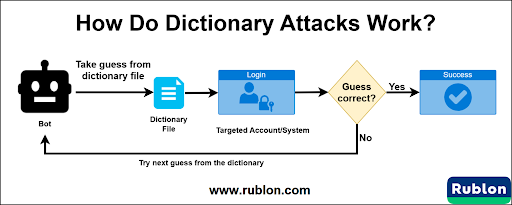
\includegraphics[scale=0.6]{pic/dictionary.png}
    \caption{Cách cuộc tấn công Dictionary hoạt động}
\end{figure}
Loại tấn công này sử dụng một phương pháp hệ thống để phá vỡ mật khẩu. Có ba bước cơ bản để thực hiện những cuộc tấn công này một cách thành công và hiểu rõ chúng có thể hữu ích trong việc học cách ngăn chặn một cuộc tấn công từ điển.\\

Thường thì, kẻ tấn công sẽ tạo ra một danh sách trước định các mật khẩu tiềm năng - một từ điển tấn công thô mà bao gồm các kết hợp của các từ phổ biến và số.
Phần mềm tự động sau đó sử dụng từ điển tấn công này để thử tấn công vào các tài khoản trực tuyến.\cite{bovsnjak2018brute}
Sau khi cuộc tấn công từ điển đã thành công tấn công vào một tài khoản dễ bị tấn công, kẻ tấn công sử dụng bất kỳ dữ liệu nhạy cảm nào được lưu trữ trong hồ sơ cho mục đích của riêng họ. Điều này có thể là để gian lận, thực hiện hành động độc hại, hoặc đơn giản là truy cập vào các tài khoản với mục đích tài chính.\\

Để biên soạn danh sách các mật khẩu tiềm năng, kẻ tấn công thường sử dụng tên thú nuôi phổ biến, nhân vật văn hóa đại chúng nhận dạng hoặc các đội thể thao và vận động viên nổi tiếng, ví dụ. Điều này là do nhiều người sử dụng loại từ này để tạo ra các mật khẩu có ý nghĩa với họ và mà họ có thể nhớ dễ dàng. Danh sách thường sẽ bao gồm các biến thể của chúng, như các kết hợp từ khác nhau, hoặc sự thêm vào của các ký tự đặc biệt.\\

Chạy danh sách này với các công cụ tự động cũng làm cho cuộc tấn công từ điển trở nên dễ dàng thành công hơn. Sử dụng danh sách mật khẩu và công cụ tự động cùng nhau khiến việc cố gắng phá vỡ mật khẩu và tấn công vào một tài khoản trực tuyến nhanh chóng hơn đáng kể. Nếu việc này được thực hiện thủ công thì cuộc tấn công sẽ mất quá nhiều thời gian và cho phép chủ sở hữu tài khoản hoặc quản trị hệ thống phát hiện và triển khai một phòng thủ chống lại cuộc tấn công.\\

Bởi vì cách chúng hoạt động, những cuộc tấn công từ điển thường không có một mục tiêu cá nhân. Thay vào đó, chúng được thực hiện với hi vọng một trong số các mật khẩu trên danh sách sẽ chính xác. Tuy nhiên, nếu kẻ tấn công đang nhắm vào một địa điểm hoặc tổ chức cụ thể, họ sẽ tạo ra một danh sách từ cụ thể và cục bộ hơn. Ví dụ, nếu họ có kế hoạch thực hiện cuộc tấn công ở Tây Ban Nha, họ có thể sử dụng các từ Tây Ban Nha phổ biến thay vì tiếng Anh. Hoặc, nếu họ đang nhắm vào một tổ chức cụ thể, họ có thể sử dụng các từ liên quan đến công ty đó.
\subsubsection{Nguyên nhân người dùng bị tấn công Dictionary}

\begin{itemize}
    \item \textbf{Sử dụng mật khẩu yếu}: Nhiều người dùng sử dụng các mật khẩu đơn giản, dễ đoán như "123456", "password", hay "abc123". Những mật khẩu này thường nằm trong danh sách từ điển mật khẩu của kẻ tấn công.
    \item \textbf{Mật khẩu phổ biến}: Có những mật khẩu phổ biến mà nhiều người dùng chọn vì dễ nhớ. Kẻ tấn công sẽ thử những mật khẩu này trước vì khả năng thành công cao hơn.
    \item \textbf{Không thay đổi mật khẩu thường xuyên}: Khi người dùng không thay đổi mật khẩu định kỳ, khả năng mật khẩu bị lộ và nằm trong danh sách từ điển của kẻ tấn công tăng lên.
    \item \textbf{Tái sử dụng mật khẩu}: Nhiều người dùng sử dụng cùng một mật khẩu cho nhiều tài khoản khác nhau. Nếu một tài khoản bị lộ, các tài khoản khác cũng có nguy cơ bị tấn công.
    \item \textbf{Thiếu ký tự đặc biệt và độ dài mật khẩu}: Mật khẩu ngắn và thiếu ký tự đặc biệt (chữ hoa, chữ thường, số, ký tự đặc biệt) dễ bị bẻ khóa hơn vì có ít sự kết hợp để thử.
    \item \textbf{Thông tin cá nhân trong mật khẩu}: Sử dụng thông tin cá nhân như tên, ngày sinh, hoặc số điện thoại làm mật khẩu khiến mật khẩu dễ bị đoán ra.
    \item \textbf{Không sử dụng xác thực hai yếu tố (2FA)}: Thiếu các biện pháp bảo vệ bổ sung như xác thực hai yếu tố làm cho việc bẻ khóa mật khẩu dễ dàng hơn.
\end{itemize}
\subsubsection{ Các công cụ dùng trong tấn công}
\begin{itemize}
    \item \textbf{John the Ripper}: Đây là một trong những công cụ bẻ khóa mật khẩu phổ biến nhất. Nó hỗ trợ nhiều định dạng mật khẩu và có thể sử dụng các tập tin từ điển để thử các mật khẩu phổ biến.
    \item \textbf{Hashcat}: Đây là một công cụ mạnh mẽ hỗ trợ bẻ khóa mật khẩu sử dụng GPU, giúp tăng tốc độ tấn công. Hashcat có thể thực hiện nhiều loại tấn công, bao gồm tấn công từ điển.
    \item \textbf{Aircrack-ng}: Bộ công cụ này thường được sử dụng để kiểm tra bảo mật mạng Wi-Fi. Nó có thể thực hiện tấn công từ điển để bẻ khóa mật khẩu WPA và WPA2.
    \item \textbf{Hydra}: Đây là một công cụ rất mạnh mẽ cho các tấn công Brute Force và từ điển trên các giao thức mạng. Nó hỗ trợ nhiều giao thức như FTP, HTTP, SMB, và nhiều hơn nữa.
    \item \textbf{Cain \& Abel}: Đây là một công cụ phục hồi mật khẩu dành cho Windows, hỗ trợ nhiều kỹ thuật bẻ khóa mật khẩu khác nhau, bao gồm tấn công từ điển.
    \item \textbf{Medusa}: Một công cụ tấn công mật khẩu dựa trên từ điển và Brute Force. Medusa được thiết kế để kiểm tra bảo mật mật khẩu trên nhiều giao thức.
    \item \textbf{THC Hydra}: Đây là một công cụ mạng mạnh mẽ để thực hiện tấn công mật khẩu từ điển. Hydra có khả năng tấn công nhiều giao thức khác nhau, từ SSH đến Telnet.
    \item \textbf{Ophcrack}: Một công cụ chuyên dụng cho việc bẻ khóa mật khẩu Windows sử dụng các bảng rainbow (rainbow tables), nhưng cũng có thể sử dụng từ điển mật khẩu để thực hiện tấn công từ điển.
    \item \textbf{Patator}: Đây là một công cụ tấn công mật khẩu đa năng, hỗ trợ nhiều loại tấn công khác nhau, bao gồm tấn công từ điển trên các dịch vụ như SSH, FTP, HTTP, và nhiều hơn nữa.
\end{itemize}
\subsection{Man in the Middle (MITM)}

\subsubsection{Tấn công MITM là gì?}
    Cuộc tấn công giữa chừng (MITM) là một thuật ngữ chung khi thủ phạm tự đặt mình vào cuộc trò chuyện giữa người dùng và ứng dụng để nghe trộm hoặc mạo danh một trong các bên hoặc cũng có thể chặn lưu lượng truy cập thậm chí có thể chặn liên lạc giữa hai máy, khiến cuộc trò chuyện có vẻ như là một cuộc trao đổi thông tin bình thường đang được tiến hành.
    
Mục tiêu của cuộc tấn công là đánh cắp thông tin cá nhân, chẳng hạn như thông tin đăng nhập, chi tiết tài khoản và số thẻ tín dụng. Mục tiêu thường là người dùng các ứng dụng tài chính, doanh nghiệp SaaS, trang web thương mại điện tử và các trang web khác yêu cầu đăng nhập.

Thông tin thu được trong một cuộc tấn công có thể được sử dụng cho nhiều mục đích, bao gồm đánh cắp danh tính, chuyển tiền không được phê duyệt hoặc thay đổi mật khẩu bất hợp pháp.

Ngoài ra, nó có thể được sử dụng để giành được chỗ đứng bên trong vành đai an toàn trong giai đoạn xâm nhập của một  cuộc tấn công có mối đe dọa dai dẳng  (APT) nâng cao.
\begin{figure}[H]
    \centering
    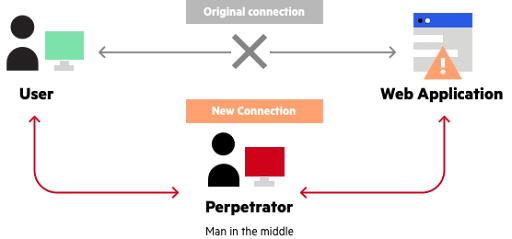
\includegraphics[scale=0.7]{pic/huê/mitm.png}
    
    \caption{Tấn công MITM}
\end{figure}
Nói rộng hơn, một cuộc tấn công MITM tương đương với việc một người đưa thư mở bảng sao kê ngân hàng của bạn, viết chi tiết tài khoản của bạn rồi dán lại phong bì và chuyển nó đến tận nhà bạn.
\subsubsection{Các kiểu tấn công MITM}
Cuộc tấn công trung gian trong an ninh mạng được coi là bất kỳ trường hợp nào mà tác nhân đe dọa đặt mình vào giữa người dùng và một thực thể như mạng, trang web hoặc ứng dụng để lấy thông tin. Phương pháp mà tin tặc lấy được thông tin đó khác nhau bằng cách sử dụng các hình thức giả mạo khác nhau, một phương pháp mạo danh các thực thể hoặc trang web trực tuyến đáng tin cậy. Các loại tấn công MITM chính bao gồm:
\begin{itemize}
    \item Giả mạo IP: Tội phạm mạng thay đổi địa chỉ Giao thức Internet (IP) của trang web, địa chỉ email hoặc thiết bị và giả mạo thực thể—khiến người dùng nghĩ rằng họ đang tương tác với một nguồn đáng tin cậy trong khi họ thực sự đang chuyển thông tin cho một tác nhân độc hại.
    \item Giả mạo DNS: Đối với giả mạo Hệ thống tên miền (DNS), kẻ gửi thư rác tạo và vận hành một trang web giả mạo mà người dùng quen thuộc và định tuyến chúng đến trang web đó để lấy thông tin xác thực của người dùng hoặc thông tin khác.
    \item Giả mạo HTTPS: Người dùng cho rằng một trang web có Bảo mật Giao thức Truyền Siêu Văn bản (HTTPS), nghĩa là họ đã mã hóa dữ liệu máy tính của mình vào máy chủ lưu trữ trang web. Tuy nhiên, chúng đã được bí mật chuyển hướng đến một trang web HTTP không an toàn, cho phép bọn tội phạm theo dõi các tương tác và đánh cắp thông tin.
\item Chiếm đoạt email: Những kẻ tấn công bí mật truy cập vào tài khoản email của ngân hàng hoặc công ty phát hành thẻ tín dụng để theo dõi các giao dịch và đánh cắp thông tin. Họ cũng có thể sử dụng tài khoản email hoặc địa chỉ email giả mạo hơi khác so với địa chỉ thực tế để cung cấp hướng dẫn sai cho khách hàng, chẳng hạn như chuyển tiền vào tài khoản séc mới.
\item Wifi Eavesdropping: Người gửi thư rác tạo các mạng Wi-Fi công cộng hoặc các điểm phát sóng có vẻ như là một doanh nghiệp lân cận hoặc nguồn đáng tin cậy khác. Người dùng kết nối sau đó sẽ bị chặn tất cả hoạt động và dữ liệu nhạy cảm của họ.
\item Tấn công SSL: Một phần mở rộng của hoạt động giả mạo HTTPS, chiếm quyền điều khiển Lớp cổng bảo mật (SSL) là khi tin tặc lấy giao thức này chịu trách nhiệm mã hóa các kết nối HTTPS và chặn dữ liệu người dùng di chuyển giữa họ và máy chủ mà họ đang kết nối.
\item Chiếm quyền điều khiển phiên: Thường được gọi là hành vi trộm cắp cookie trình duyệt, kẻ tấn công sẽ đánh cắp thông tin được lưu trữ trên cookie trình duyệt web, chẳng hạn như mật khẩu đã lưu.
\end{itemize}
\subsubsection{Tiến trình tấn công MITM}
Việc thực thi MITM thành công có hai giai đoạn riêng biệt: Chặn và Giải mã.
\begin{itemize}
    \item Chặn:\\
    Bước đầu tiên chặn lưu lượng truy cập của người dùng qua mạng của kẻ tấn công trước khi nó đến đích dự định.
    
Cách phổ biến nhất (và đơn giản nhất) để thực hiện việc này là tấn công thụ động, trong đó kẻ tấn công cung cấp các điểm truy cập WiFi độc hại, miễn phí cho công chúng. Thường được đặt tên theo cách tương ứng với vị trí của chúng, chúng không được bảo vệ bằng mật khẩu. Khi nạn nhân kết nối với một điểm phát sóng như vậy, kẻ tấn công sẽ có được khả năng hiển thị đầy đủ đối với bất kỳ hoạt động trao đổi dữ liệu trực tuyến nào.

Những kẻ tấn công muốn thực hiện một cách tiếp cận tích cực hơn để đánh chặn có thể thực hiện một trong các cuộc tấn công sau:
\begin{itemize}
    \item Giả mạo IP  liên quan đến kẻ tấn công cải trang thành một ứng dụng bằng cách thay đổi tiêu đề gói trong địa chỉ IP. Kết quả là người dùng cố gắng truy cập URL được kết nối với ứng dụng sẽ được gửi đến trang web của kẻ tấn công.
    \item Giả mạo ARP  là quá trình liên kết địa chỉ MAC của kẻ tấn công với địa chỉ IP của người dùng hợp pháp trên mạng cục bộ bằng cách sử dụng tin nhắn ARP giả mạo. Do đó, dữ liệu do người dùng gửi đến địa chỉ IP máy chủ thay vào đó sẽ được truyền đến kẻ tấn công.

\item Giả mạo DNS , còn được gọi là đầu độc bộ đệm DNS, liên quan đến việc xâm nhập vào máy chủ DNS và thay đổi bản ghi địa chỉ của trang web. Kết quả là, người dùng cố gắng truy cập trang web sẽ được bản ghi DNS đã thay đổi gửi đến trang web của kẻ tấn công.

\end{itemize}
\item Giải mã:\\
Sau khi chặn, mọi lưu lượng SSL hai chiều cần được giải mã mà không thông báo cho người dùng hoặc ứng dụng. Một số phương pháp tồn tại để đạt được điều này:
\begin{itemize}
    \item Việc giả mạo HTTPS  gửi chứng chỉ giả mạo đến trình duyệt của nạn nhân sau khi yêu cầu kết nối ban đầu tới một trang web an toàn được thực hiện. Nó chứa dấu vân tay kỹ thuật số liên quan đến ứng dụng bị xâm nhập mà trình duyệt sẽ xác minh theo danh sách các trang web đáng tin cậy hiện có. Kẻ tấn công sau đó có thể truy cập bất kỳ dữ liệu nào do nạn nhân nhập trước khi nó được chuyển đến ứng dụng.

\item SSL BEAST  (khai thác trình duyệt chống lại SSL/TLS) nhắm vào lỗ hổng TLS phiên bản 1.0 trong SSL. Tại đây, máy tính của nạn nhân bị nhiễm JavaScript độc hại có chức năng chặn các cookie được mã hóa được gửi bởi một ứng dụng web. Sau đó, chuỗi khối mật mã (CBC) của ứng dụng bị xâm phạm để giải mã cookie và mã thông báo xác thực của ứng dụng.

\item Việc chiếm quyền điều khiển SSL  xảy ra khi kẻ tấn công chuyển các khóa xác thực giả mạo cho cả người dùng và ứng dụng trong quá trình bắt tay TCP. Điều này thiết lập những gì có vẻ là một kết nối an toàn trong khi trên thực tế, người đàn ông ở giữa kiểm soát toàn bộ phiên.
\item  Việc loại bỏ SSL  hạ cấp kết nối HTTPS xuống HTTP bằng cách chặn xác thực TLS được gửi từ ứng dụng tới người dùng. Kẻ tấn công gửi phiên bản không được mã hóa của trang web ứng dụng cho người dùng trong khi vẫn duy trì phiên bảo mật với ứng dụng. Trong khi đó, kẻ tấn công có thể nhìn thấy toàn bộ phiên của người dùng.
\end{itemize}
\end{itemize}
\subsubsection{Mức độ phổ biến của các cuộc tấn công Man-In-The-Middle}
Các cuộc tấn công MITM rất phổ biến, mặc dù không đến mức Ransomware hoặc lừa đảo. Các kiểu tấn công này rất dễ thực hiện và các công cụ hack được cung cấp công khai. Chúng được thực hiện không chỉ từ bên ngoài, mà còn có những sự cố bên trong tổ chức nơi MITM được sử dụng để tấn công mạng nội bộ.
\newline
Thật không may, những loại sự cố này rất khó phát hiện, đó là lý do tại sao hành động ngăn chặn là rất quan trọng, đồng thời cũng giúp cải thiện an ninh mạng và quyền riêng tư.

\subsubsection{Các công cụ được sử dụng }
\begin{itemize}
    \item \textbf{Windows}: Ví dụ, Cain và Abel – không sử dụng, nhưng nó có vẻ là một công cụ mạnh mẽ để lấy mật khẩu trên mạng.
    \item \textbf{Android}: cSploit. Là một ứng dụng mã nguồn mở được phát triển cho điện thoại Android. Để bắt đầu chạy nó, bạn phải có đặc quyền root trên điện thoại của mình. Nó yêu cầu cho phép rất nhiều và hoạt động của nó chỉ đơn giản là chọn từ menu những gì chúng ta muốn làm – thay thế hình ảnh, kiểm tra lưu lượng mạng hoặc giải mã các gói đã gửi.
    \item \textbf{Linux}: Kali Linux là một bản phân phối Linux dành cho tin tặc.
\end{itemize}
\subsubsection{Biện pháp bảo vệ và ngăn chặn}
\begin{figure}[H]
    \centering
    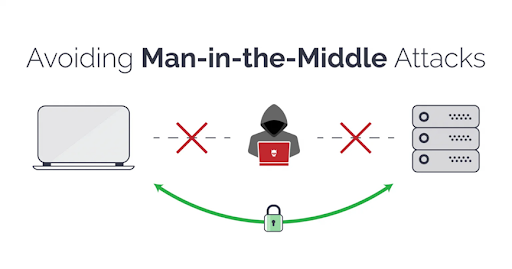
\includegraphics[scale=0.8]{pic/huê/tấn công mitm.png}
    
    \caption{Bảo vệ và ngăn chặn tấn công MITM}
\end{figure}
Việc ngăn chặn tấn công MITM yêu cầu một số bước nhất định từ người dùng. Cùng với đó là kết hợp các phương thức mã hóa và xác minh khác. Do đó để bảo vệ và ngăn chặn tấn công cần có sự kết hợp giữa người dùng và quản trị viên:
\begin{itemize}
    \item  Đối với người dùng:

\begin{itemize}
    \item Tránh các kết nối WiFi không được bảo vệ bằng password, vì chúng dễ bị tấn công và bị tội phạm mạng đánh cắp dữ liệu.
    \item Chú ý đến các thông báo của trình duyệt về trang web không an toàn.\cite{ylli2021man}
\item Đăng xuất khỏi các ứng dụng không không sử dụng nữa.
\item  Không sử dụng mạng công cộng (ở quán cafe, cửa hàng, khách sạn…) khi thực hiện các giao dịch nhạy cảm.

\item  Tránh email lừa đảo: Tội phạm mạng thường tạo ra các email lừa đảo để lừa người dùng mở chúng. Người dùng cần cân nhắc kỹ trước khi mở email đến từ nguồn không xác minh hoặc không rõ. Thông thường, email lừa đảo sẽ giả mạo một nguồn đáng tin cậy, như một tài khoản ngân hàng hoặc một tổ chức tài chính. Những email này thường yêu cầu người dùng nhấp vào liên kết để nhập thông tin đăng nhập hoặc cập nhật mật khẩu. Tuyệt đối tránh nhấp vào các liên kết này, vì chúng có thể chuyển hướng người dùng đến trang web giả mạo hoặc tải xuống phần mềm độc hại \cite{ylli2021man}.
\end{itemize}
\item  Đối với quản trị viên:
\begin{itemize}
    \item Tạo kết nối bảo mật: Bước đầu tiên để chống lại các cuộc tấn công MitM là đảm bảo kết nối an toàn. Người dùng chỉ nên truy cập các trang web hiển thị “HTTPS” trong thanh địa chỉ URL, thay vì chỉ “HTTP”. Hầu hết các trình duyệt web hiển thị biểu tượng ổ khóa trước URL để chỉ ra rằng trang web là an toàn. Việc này sẽ giúp giảm thiểu tấn công giả mạo bằng cách mã hóa và xác thực dữ liệu. Quản trị viên nên áp dụng việc xác thực đa yếu tố cho tất cả người dùng, để tăng cường thêm một lớp bảo mật cho việc truyền thông trực tuyến \cite{ylli2021man}.
\item Sử dụng mã hóa mạng riêng ảo (VPN): VPN mã hóa kết nối internet và truyền dữ liệu trực tuyến như mật khẩu và thông tin thẻ tín dụng, và nên được sử dụng khi kết nối đến các mạng Wi-Fi công cộng và điểm phát sóng không an toàn. VPN có thể ngăn chặn tiềm năng các cuộc tấn công MitM. Ngay cả khi tội phạm mạng có thể truy cập vào mạng, họ cũng sẽ không thể giải mã các tin nhắn hoặc truy cập tài nguyên do mã hóa bởi VPN cung cấp. Tổ chức cũng cần đảm bảo nhân viên đăng nhập hệ thống qua mạng riêng ảo của công ty, đặc biệt khi làm việc từ xa \cite{ylli2021man}.
\item  Bảo vệ điểm cuối: Triển khai bảo mật điểm cuối toàn diện là rất quan trọng khi cố gắng ngăn chặn sự lan truyền của phần mềm độc hại và các cuộc tấn công mạng khác. Vì các cuộc tấn công MitM thường sử dụng phần mềm độc hại để thực hiện, việc cài đặt sản phẩm chống phần mềm độc hại và bảo mật internet là hết sức quan trọng.
\end{itemize}
\end{itemize}
\subsection{Tấn công Kết hợp Plaintext-Ciphertext (Known- Plaintext Attack)
}
\subsubsection{Know-Plaintext Attack là gì?}
Known-plaintext attacks (KPA) là khi tin tặc sử dụng bản rõ và bản mã để xác định thuật toán hoặc khóa mã hóa.

Trong một Known-plaintext Attacks, kẻ tấn công có quyền truy cập vào cả dạng mã hóa của dữ liệu (ciphertext) và bản sao văn bản gốc tương ứng của dữ liệu gốc (unencrypted form). Kẻ tấn công cố gắng xác định khóa hoặc thuật toán mã hóa bằng cách kiểm tra mối quan hệ giữa plaintext và ciphertext.

Ví dụ: nếu “CRYPTO” được mã hóa thành “XUZZA”, việc biết cặp này có thể cho phép kẻ tấn công giải mã các phần khác của tin nhắn cũng được mã hóa bằng cùng một khóa thay thế. Điều này chứng tỏ rằng, với một số thuật toán mã hóa, ngay cả một lượng kiến thức nhỏ cũng có thể dẫn đến việc giải mã rộng hơn.

Kiểu tấn công này sử dụng một lỗ hổng trong kỹ thuật mã hóa giúp xác định các mẫu hoặc kết nối được tạo ra giữa bản rõ và bản mã. Nếu không được ngăn chặn một cách chính xác, các Known-plaintext Attacks có thể gây nguy hiểm cho tính bảo mật của hệ thống mã hóa.

Hai phương pháp phổ biến để khai thác plaintext và dạng mã hóa tương ứng của nó nhằm khám phá các khóa mã hóa bao gồm phân tích tần số (frequency analysis) và khớp mẫu (pattern matching). Phương pháp phân tích tần số sử dụng các phương pháp mã hóa đơn giản bằng cách thay thế từng ký tự hoặc ký hiệu một-một. Những kẻ tấn công có thể tìm ra chìa khóa hoặc mở khóa phần còn lại của giao tiếp bằng cách so sánh tần suất xuất hiện của các chữ cái hoặc mẫu cụ thể trong plaintext và bản mã liên quan.

Những kẻ tấn công có thể phát hiện ra các xu hướng khi cùng một plaintext tạo ra cùng một bản mã theo phương pháp khớp mẫu. Họ có thể nhận ra thuật toán mã hóa và giải mã toàn bộ tin nhắn bằng cách xác định các mẫu trong văn bản được mã hóa và so sánh chúng với các mẫu đã biết trong plaintext gốc.

\begin{figure}[H]
    \centering
    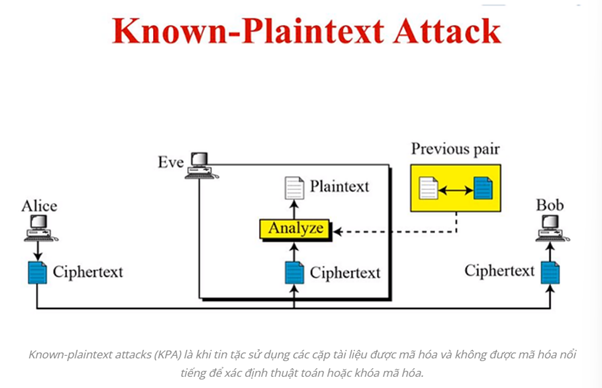
\includegraphics[scale=0.9]{pic/huê/kpa.png}
    
    \caption{Tấn công Know-Plaintext}
\end{figure}
\subsubsection{KPA đã hoạt động như nào?
}
Trong KPA, kẻ tấn công có thể tìm hiểu các chi tiết quan trọng về phương pháp mã hóa bằng cách phân tích cách các đoạn cụ thể của văn bản gốc được chuyển đổi thành văn bản mã hóa bằng cách sử dụng cùng một khóa hoặc thuật toán mã hóa.

Cuộc tấn công bao gồm các bước sau:
\begin{itemize}
    \item \textbf{Thu thập các cặp đã biết:}
Kẻ tấn công tích lũy các cặp plaintext và văn bản mật mã được mã hóa liên quan có được thông qua các kỹ thuật khác nhau, chẳng hạn như thông tin liên lạc bị chặn hoặc rò rỉ dữ liệu.
\item \textbf{Phân tích mẫu:}
Khi bản rõ được mã hóa để tạo thành bản mã, kẻ tấn công sẽ so sánh các mẫu, sửa đổi và biến đổi diễn ra. Để hiểu hoạt động của quá trình mã hóa, họ tìm kiếm các mối quan hệ thường xuyên giữa plaintext và ciphertext đã biết.
\item \textbf{Lấy khóa hoặc thuật toán:}
Kẻ tấn công cố gắng xác định các yếu tố mã hóa quan trọng, chẳng hạn như khóa mã hóa, thuật toán hoặc các tham số quy trình khác, dựa trên các mẫu mà chúng đã nhận thấy. Họ có thể sao chép độc lập quá trình mã hóa nhờ vào suy luận này.
\item \textbf{Giải mã dữ liệu khác:}
Kẻ tấn công có thể giải mã các tài liệu được mã hóa khác sử dụng cùng một thuật toán mã hóa bằng cách sử dụng khóa hoặc thuật toán được suy luận. Quy trình này có thể làm rò rỉ thông tin bí mật hoặc gây nguy hiểm cho tính bảo mật của hệ thống mã hóa.

\end{itemize}
\subsubsection{Biện pháp bảo vệ và ngăn chặn}
Để bảo vệ chống lại các Known-plaintext Attacks, hãy áp dụng thuật toán mã hóa mạnh, quản lý khóa mã hóa một cách an toàn, sử dụng khóa duy nhất cho mỗi phiên và thêm tính ngẫu nhiên vào quy trình mã hóa để tăng cường khả năng bảo vệ chống lại các cuộc tấn công.
\begin{itemize}
    \item \textbf{Áp dụng thuật toán mã hóa mạnh:} Bằng cách ngăn chặn các mẫu trong bản rõ tương quan với các mẫu trong văn bản mã hóa, các thuật toán mã hóa hiện đại như Tiêu chuẩn mã hóa nâng cao (AES) được tạo ra để tồn tại trước các cuộc tấn công như vậy. AES là một thuật toán mã hóa đối xứng được sử dụng rộng rãi, nổi tiếng về tính bảo mật và hiệu quả.
\item \textbf{Quản lý an toàn các khóa mã hóa:} Bằng cách quản lý an toàn  ta có thể  tránh truy cập trái phép. Sử dụng kho lưu trữ khóa an toàn, xoay khóa thường xuyên và sử dụng các kỹ thuật tạo khóa mạnh mẽ. Ngoài ra, tránh mã hóa các khối dữ liệu rời rạc, có thể dự đoán được. Để ngăn kẻ tấn công sử dụng các cặp đã biết, hãy mã hóa toàn bộ tin nhắn hoặc tệp.
\item \textbf{Sử dụng khóa duy nhất cho mỗi phiên:} sử dụng các phím khác nhau cho các phiên và nỗ lực khác nhau. Tác động của Known-plaintext Attacks đã giảm do mỗi phiên sẽ sử dụng một khóa mã hóa khác nhau. Ngoài ra, hãy duy trì các phiên bản mới nhất của hệ thống, thư viện và phần mềm mã hóa của bạn. Các bản sửa lỗi bảo mật giúp sửa chữa các lỗ hổng thường được đưa vào các bản cập nhật.
\item  \textbf{Thêm tính ngẫu nhiên vào quy trình mã hóa:} Trước khi mã hóa bản rõ của dữ liệu, hãy thêm một giá trị ngẫu nhiên vào đó. Điều này làm cho mỗi mã hóa là duy nhất, ngay cả khi mã hóa cùng một bản rõ nhiều lần. Ngoài ra, hãy tránh các phương pháp mã hóa được biết là dễ bị tấn công bằng plaintext đã biết. Điều đó nói rằng, hãy thực hiện thẩm định thích hợp khi chọn thuật toán mã hóa.

\end{itemize}
\subsection{Tấn công Chọn văn bản (Chosen-Plaintext Attack)}
\subsubsection{Chosen-Plaintext Attack là gì?}
Tấn công bằng văn bản gốc được chọn là phương pháp mà tin tặc sử dụng để phá mã bí mật hoặc hệ thống mã hóa nhằm có được quyền truy cập trái phép vào thông tin. Trong cuộc tấn công này, tin tặc có thể chọn các tin nhắn cụ thể (bản rõ) để mã hóa bằng thuật toán mã hóa của mục tiêu. Làm như vậy sẽ tạo ra các bản mã tương ứng (phiên bản được mã hóa của bản rõ). Tin tặc phân tích các bản mã để tiết lộ toàn bộ hoặc một phần khóa mã hóa bí mật. Cuộc tấn công này nhằm mục đích thu thập thông tin có thể được sử dụng để giải mã các tin nhắn trong tương lai và xâm phạm tính bảo mật của hệ thống \cite{nordvpn-2024}.
\subsubsection{Tiến trình công cuộc tấn công}
\begin{itemize}
    \item Kẻ tấn công chọn bản rõ mà chúng muốn mã hóa bằng thuật toán hoặc hệ thống mã hóa mục tiêu.\cite{nordvpn-2024}
    \item Các bản rõ đã chọn sẽ được mã hóa bằng thuật toán mã hóa đích, tạo ra các bản mã tương ứng. Kẻ tấn công có thể tìm ra thuật toán mã hóa mục tiêu thông qua kiến thức công cộng hoặc kỹ thuật đảo ngược \cite{nordvpn-2024}.
    \item Kẻ tấn công quan sát và ghi lại các bản mã được tạo ra cho các bản rõ đã chọn \cite{nordvpn-2024}.
    \item Phân tích mối quan hệ giữa các bản rõ đã chọn và các bản mã tương ứng để xác định các mẫu hoặc lỗ hổng trong thuật toán mã hóa \cite{nordvpn-2024}.
    \item Dựa trên phân tích, kẻ tấn công có thể cố gắng tìm hiểu thêm về khóa bí mật hoặc khai thác bất kỳ điểm yếu nào được phát hiện trong quá trình mã hóa \cite{nordvpn-2024}.
    \item Nếu cần, kẻ tấn công có thể lặp lại các bước trên với các bản rõ được chọn bổ sung để thu thập thêm thông tin \cite{nordvpn-2024}.
\end{itemize}
\subsubsection{Các kiểu tấn công CPA}
\begin{itemize}
    \item \textbf{Batch chosen plaintext attack}: Tấn công hàng loạt bản rõ được chọn cho phép kẻ tấn công xử lý nhiều bản rõ cùng một lúc \cite{nordvpn-2024}.
    \item \textbf{Adaptive chosen plaintext attack}. Trong cuộc tấn công này, kẻ tấn công có thể tự động điều chỉnh các bản rõ đã chọn dựa trên phản hồi nhận được từ hệ thống mã hóa \cite{nordvpn-2024}.
\end{itemize}
\subsubsection{Nơi có thể xảy ra tấn công CPA}
\begin{itemize}
    \item Các giao thức mã hóa. Các cuộc tấn công bằng văn bản gốc được chọn có thể nhắm mục tiêu vào các giao thức mã hóa (ví dụ: liên lạc an toàn, trao đổi khóa hoặc xác thực). Bằng cách thao tác các bản rõ đã chọn trong quá trình thực thi giao thức, kẻ tấn công có thể hiểu rõ hơn về các lỗ hổng bảo mật của giao thức hoặc truy cập thông tin nhạy cảm \cite{nordvpn-2024}.
    \item An ninh mạng. Các cuộc tấn công bằng văn bản gốc được chọn có thể nhắm mục tiêu vào các hệ thống mật mã bảo vệ thông tin liên lạc trên mạng, chẳng hạn như VPN (mạng riêng ảo) \cite{nordvpn-2024}.
\end{itemize}
\subsubsection{Chosen-plaintext Attacks và Known-plaintext Attacks}
Chosen-plaintext Attacks liên quan đến việc đối thủ chọn bản rõ và phân tích bản mã tương ứng, trong khi Known-plaintext Attacks xảy ra khi kẻ tấn công sở hữu một phần kiến thức về bản rõ \cite{hoang-2023}.\\
Hiểu được sự khác biệt giữa hai cuộc tấn công mật mã này là rất quan trọng đối với các chiến lược bảo vệ mật mã hiệu quả \cite{hoang-2023}.
\begin{table}[H]
\resizebox{\textwidth}{!}{%
\begin{tabular}{|l|l|l|}
\hline
                                             & \textbf{Chosen-plaintext Attacks}      & \textbf{Known-plaintext Attacks}       \\ \hline
\multicolumn{1}{|l|}{\textbf{Bối cảnh}} &
  \multicolumn{1}{l|}{Kẻ tấn công lựa chọn plaintext} &
  \multicolumn{1}{l|}{Kẻ tấn công chỉ biết một vài plaintext} \\ \hline
\multicolumn{1}{|l|}{\textbf{Loại Attack}}   & \multicolumn{1}{l|}{Nghe lén thụ động} & \multicolumn{1}{l|}{Thao tác chủ động} \\ \hline
\multicolumn{1}{|l|}{\textbf{Loại hình}} &
  \multicolumn{1}{l|}{Giải mã văn bản mật mã} &
  \multicolumn{1}{l|}{Xác định phương pháp mã hoá} \\ \hline
\multicolumn{1}{|l|}{\textbf{Trình độ hiểu biết cần có}} &
  \multicolumn{1}{l|}{Không yêu cầu có hiểu biết về plaintext} &
  \multicolumn{1}{l|}{Một số plaintext cần hiểu rõ} \\ \hline
\multicolumn{1}{|l|}{\textbf{Tính phức tạp}} & \multicolumn{1}{l|}{Vừa phải}          & \multicolumn{1}{l|}{Thấp}              \\ \hline
\textbf{Ví dụ}                               & Giải mã cổ điển                        & Phân tích tần số                       \\ \hline
\end{tabular}%
}
\end{table}
Phân tích tần số tập trung vào việc kiểm tra sự xuất hiện của các chữ cái hoặc ký hiệu để xác định thuật toán mã hóa, không giống như phân tích mật mã cổ điển, kiểm tra văn bản mã hóa để tìm các mẫu và sai sót.
\subsubsection{Biện pháp bảo vệ và ngăn chặn tấn công}
\begin{itemize}
    \item Để ngăn chặn các cuộc tấn công bằng văn bản gốc đã chọn, điều cần thiết là sử dụng các khóa mã hóa mạnh được tạo ngẫu nhiên, đủ dài, được lưu trữ an toàn và đảm bảo chỉ những người dùng được ủy quyền mới có thể truy cập chúng.
    \item Các khóa không được sử dụng lại hoặc chia sẻ trên các hệ thống hoặc giao thức mã hóa khác nhau. \item Chìa khóa cũng cần được thay thường xuyên và vứt bỏ sau khi sử dụng. 
    \item Hơn nữa, điều cần thiết là phải sử dụng các thuật toán và chế độ mã hóa an toàn để đảm bảo tính bảo mật và tính toàn vẹn. Các thuật toán mã hóa được kiểm duyệt kỹ lưỡng sẽ trải qua quá trình thử nghiệm rộng rãi để chống lại các cuộc tấn công đã biết, bao gồm cả Chosen Plaintext Attack, chẳng hạn như AES-GCM hoặc ChaCha20-Poly1305. Các thuật toán và chế độ này sử dụng thẻ xác thực và mã hóa không dựa trên cơ sở để ngăn chặn các cuộc tấn công bằng văn bản gốc đã chọn.
\end{itemize}
\subsection{Tấn công Timing Attack}
\subsubsection{Tấn công Timing Attack là gì?}
\begin{itemize}
    \item Là một dạng tấn công thuộc loại side-channel mà hacker dựa vào thông tin phân tích được từ thời gian thực thi một đoạn logic từ hệ thống từ đó truy ra dần kết quả sau cùng, có thể xem Timing Attack là một dạng \textit{manual brute force} cũng được, vì cùng một cách thức để truy ra kết quả, nhưng khác là hacker cần đầu tư nhiều hơn để phân tích dữ liệu đang có để cho ra input tiếp theo \cite{trinh-2023}.
    \item Hacker luôn cố gắng lợi dụng bản năng của người lập trình viên, luôn muốn code của mình chạy càng nhanh càng tốt, để thực hiện ý đồ tấn công. Kẻ tấn công có thể bắt đầu với phỏng đoán (giả thiết) bit đầu tiên có thể là 0 hoặc là 1. Sau đó xem xét các kết quả giả thiết trong mối tương quan chặt chẽ giữa thời gian thực thi thực tế và thời gian dự đoán. Quá trình này được thực hiện nhiều lần, cho đến khi kẻ tấn công tìm ra được hết các bit khóa bằng cách quan sát sự tương quan về mặt thời gian giữa nhiều mẫu và bit khóa lựa chọn. Như vậy không gian tìm kiếm khóa có thể đã được thu nhỏ lại tấn công này được cho là khá đơn giản về mặt tính toán \cite{trinh-2023}.
\end{itemize}
\underline{\textbf{Ví dụ thực tế:}}\\
Đối với lập trình viên, chúng ta sẽ phải gặp trường hợp cần xác thực request đến từ phía client, hay server to server. Có rất nhiều cách để triển khai, thông thường là sử dụng JWT, Oauth2, OpenID Connect hay sử dụng bên thứ 3 để authen như Google, Facebook, AWS Cognito... Một trong những cách phổ biến và dễ triển khai nhất là sử dụng API key.\\
Tuy nhiên APIKey vẫn có thể bị lộ bằng nhiều cách tấn công, một trong số đó là Timing attack \cite{leo-2024}.
\subsubsection{Cách thức hoạt động}
Các cuộc tấn công tính thời gian lợi dụng thực tế là các thông tin đầu vào khác nhau cho các biểu mẫu đăng nhập có thể mất lượng thời gian khác nhau để xử lý. Việc xác định thời gian đầu vào khác nhau diễn ra trong các lần thử lặp lại bắt đầu tiết lộ các mẫu mà kẻ tấn công có thể ngoại suy và xây dựng từ đó \cite{wright-2023}.\\
\indent Có một số phần tốn thời gian khác nhau trong quá trình đăng nhập. Dài nhất thường là băm mật khẩu trước khi so sánh với hàm băm được lưu trữ hiện có. Các phần khác của quy trình cũng có thể mất một lượng thời gian có thể đo lường được, chẳng hạn như xác thực tên người dùng, xác định tên người dùng đó phù hợp với người dùng hợp lệ, v.v. Băm mật khẩu nói riêng là một tác vụ có chủ đích chậm, vì vậy khá dễ dàng để phân biệt sự khác biệt giữa một lần đăng nhập yêu cầu băm mật khẩu cho phù hợp, so với mật khẩu bỏ qua mật khẩu đó \cite{wright-2023}.\\
\indent Khi một lần đăng nhập thất bại xảy ra, nó có thể xảy ra nhanh hơn nhiều so với một lần đăng nhập thành công do người dùng không có tên đã cho hoặc hàm băm mật khẩu bị bỏ qua hoặc không khớp. Chỉ cần đo thời gian thực hiện với các lần đăng nhập khác nhau, thông tin tiềm ẩn về các lần đăng nhập có thể bị rò rỉ \cite{wright-2023}.\\
\underline{Các ví dụ về cách thức tấn công Timing Attack:}
\begin{itemize}
    \item Đoán mật khẩu : Kẻ tấn công có thể sử dụng Timing Attack để đoán mật khẩu bằng cáhc đo thời gian thực hiện của chức năng xác minh mật khẩu. Kẻ tấn công gửi 1 loạt các lần đoán mật khẩu đến hàm này và đo thời gian cần thực hiện của các lần đoán khác nhau, kẻ tấn công có thể xác định lần đoán nào gần nhất với mật khẩu đúng và sử dụng lần đoán đó làm lần đoán tiếp theo. Quá trình này có thể được lặp lại cho đến khi đoán được mật khẩu chính xác \cite{cqr-2023}.
    \item Khôi phục khóa mật mã: Bằng cách đo thời gian cần thiết để thực hiện các hoạt động mã hóa hoặc giải mã. Bằng cáhc gửi một loạt thông tin đầu vào đến hệ thống và đo thời gian thực hiện các thao tác, kẻ tấn công có thể suy ra thông tin về khóa bí mật và có khả năng khôi phục nó \cite{cqr-2023}.
    \item Bỏ qua xác thực: Kẻ tấn công có thể sử dụng một cuộc tấn công Timing Attack để vượt qua hệ thống xác thực bằng cách đo thời gian cần thiết để nhận được phản hồi cho yêu cầu đăng nhập. Bằng cách gửi một loạt các lần thử đăng nhập với tên người dung và mật khẩu khác nhau, kẻ tấn công có thể đo thời gian thực thi của hệ thống xác thực và xác định tổ hợp tên người dùng và mật khẩu nào gần đúng nhất. Quá trình này có thể được lặp lại cho đến khi đoán được thông tin thực chính xác, cho phép kẻ tấn công bỏ qua hệ thống xác thực \cite{cqr-2023}.

\end{itemize}
\subsubsection{Biện pháp tấn công và ngăn chặn}
\begin{itemize}
    \item Thêm nhiễu: Thêm các khoảng thời gian ngẫu nhiên vào quá trình xử lý để làm khó việc đoán thời gian thực thi chính xác.
    \item Sử dụng thuật toán hằng thời gian: Các thuật toán mật mã được thiết kế để thực thi trong một khoảng thời gian cố định, không phụ thuộc vào giá trị của dữ liệu hoặc khóa \cite{biswas2017survey}.
    \item Kiểm tra toàn bộ dữ liệu: Đảm bảo rằng toàn bộ dữ liệu đầu vào được kiểm tra trước khi phản hồi, thay vì dừng lại ngay khi phát hiện lỗi \cite{dhem2000practical}.
    \item Triển khai các hệ thống giới hạn tốc độ có thể ngăn kẻ tấn công thu thập đủ dữ liệu để thực hiện timing attack \cite{biswas2017survey}.
    \item  Nên xác định các chức năng quan trọng về bảo mật và tạo chúng theo thời gian không đổi \cite{dhem2000practical}.
\end{itemize}

\newpage
\subsection{Tấn công Vi phân (Differential Cryptanalysis)}
Các kết quả của phần này được trích từ \cite{hey2002}.
\subsubsection{Lịch sử phát triển}
Được lần đầu công bố bởi Eli Biham và Adi Shamir vào cuối thập niên 1980 nhằm tấn công hệ mật DES, tuy nhiên có bằng chứng cho rằng IBM và NSA đã biết về cách thức tấn công này từ những năm 1970 và 1 trong những nguyên tắc S-box được thiết kế bị che giấu là nhằm chống lại dạng tấn công này.
\setstretch{1.5}
Mặc dù là phương thức tấn công hiệu quả rất nhiều hệ mật vào thời điểm ra đời, tuy nhiên người ta chỉ ra DES có khả năng chống lại dạng tấn công này hiệu quả. Để phá mã thành công DES, cần $2^{47}$ bản rõ chọn trước.

Năm 1994, một thành viên của đội thiết kế DES của công ty IBM, Don Coppersmith, công bố một bài báo đề cập rằng Tấn công Vi phân đã được biết tới bởi IBM vào đầu năm 1974, và chống lại dạng tấn công này là 1 trong những mục tiêu thiết kế của DES. Theo tác giả Steven Levy, IBM đã tự mình khám phá ra Tấn công Vi phân và NSA cũng tỏ ra rất quan tâm đến dạng tấn công này. Như Coppersmith giải thích: "Sau khi thảo luận với NSA, IBM đã quyết định rằng việc công khai nguyên lý thiết kế của DES, sẽ tiết lộ về chi tiết kỹ thuật Tấn công Vi phân, một dạng tấn công mạnh mẽ có thể dùng để chống lại rất nhiều hệ mật. Điều này sẽ làm yếu đi lợi thế cạnh tranh của Hoa Kỳ trước các quốc gia khác trong lĩnh vực Bảo mật." Với IBM, Tấn công Vi phân được biết tới với cái tên "T-attack" hay "Tickle Attack".

Trong khi DES được thiết kế với mục tiêu chống lại Tấn công Vi phân, các hệ mật khác được chứng minh là rất dễ tổn thương với dạng tấn công này. Một trường hợp có thể kể tới là Hệ mã khối FEAL. Phiên bản gốc với 4 vòng (FEAL-4) có thể bị phá vỡ sử dụng chỉ 8 bản rõ chọn trước, và thậm chí phiên bản 31 vòng của FEAL cũng dễ dàng bị phá vỡ bởi Tấn công Vi phân. Ngược lại, tiến trình tấn công phá vỡ DES cần tới $2^{47}$ bản rõ chọn trước.
\subsubsection{Nguyên lý cơ bản}
Tấn công vi phân tìm kiếm sự xuất hiện với xác suất lớn của một sai phân bản rõ và sai phân bản mã nào đó.

Giả sử có một hệ với input $X = [ X_1 X_2 ... X_n ]$ và output $Y = [Y_1 Y_2 ... Y_n].$ Xét 2 input $X^{'}, X^{"}$ của hệ với output tương ứng $Y^{'}, Y^{"}.$ 

Định nghĩa sai phân đầu vào $\Delta X = X^{'} \oplus X^{"}$, trong đó $\oplus$ là phép toán XOR, và sai phân đầu ra $\Delta Y = Y^{'} \oplus Y^{"}.$

Trong một hệ mã ngẫu nhiên lý tưởng, xác suất để một sai phân đầu ra xác định $\Delta Y$ xuất hiện tương ứng với một sai phân đầu vào $\Delta X$ cho trước là $(\frac{1}{2})^n$, với $n$ là số bit của $X$. Tấn công Vi phân tìm kiếm các cặp sai phân $(\Delta X, \Delta Y)$ mà xuất hiện với xác suất cao $p_D$, theo nghĩa là lớn hơn $(\frac{1}{2})^n$ rất nhiều.

Tấn công Vi phân là một dạng Tấn công chọn bản rõ, nghĩa là kẻ tấn công có thể chọn đầu vào và xem xét đầu ra trong việc cố gắng khôi phục lại khóa. Với tấn công vi phân, kẻ tấn công lựa chọn các cặp input $X'$ và $X''$, thỏa mãn một $\Delta X$ xác định nào đó, biết rằng với giá trị $\Delta X$ đó, một giá trị $\Delta Y$ cụ thể xuất hiện với xác suất cao.
\subsubsection{Phân tích tính chất Vi phân của S-box}
Ta sẽ phân tích tính chất Vi phân của S-box sau:
\begin{figure}[H]
    \centering
    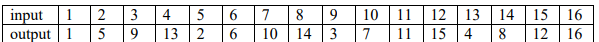
\includegraphics[scale=1]{Các công cụ và kĩ thuật sử dụng trong tấn công/S-boz.png}
    
\end{figure} 
Ta có bảng thống kê tương ứng với một số sai phân đầu vào:
\begin{figure}[H]
    \centering
    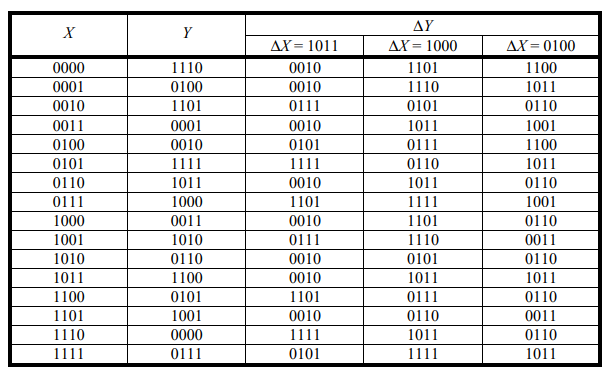
\includegraphics[scale=0.9]{Các công cụ và kĩ thuật sử dụng trong tấn công/sample diff sbox.png}
    
    \caption{Bảng thống kê tương ứng với một số sai phân đầu vào}
\end{figure}
Từ bảng trên, ta có thể thấy số lần xuất hiện của $\Delta Y = 0010$ với $\Delta X = 1011$ là 8 trên 16 giá trị có thể (tức là xác suất $\frac{8}{16}$); số lần xuất hiện của $\Delta Y = 1011$ với $\Delta X = 1000$ là 4 trên 16; số lần xuất hiện của $\Delta Y = 1010$ với $\Delta X =0100$ là 0 trên 16. 

Ta có thể tổng hợp thông tin hoàn thiện về tính chất Vi phân của 1 S-box dưới dạng một bảng Phân phối Sai phân với các hàng biểu diễn $\Delta X$ và các cột biểu diễn $\Delta Y$ (dưới dạng thập lục phân). Bảng Phân phối Sai phân của S-box đề cập ở trên được cho bởi bảng dưới đây. Mỗi phần tử trong bảng biểu diễn số lần xuất hiện của cặp sai phân $(\Delta X, \Delta Y)$ tương ứng. 
\begin{figure}[H]
    \centering
    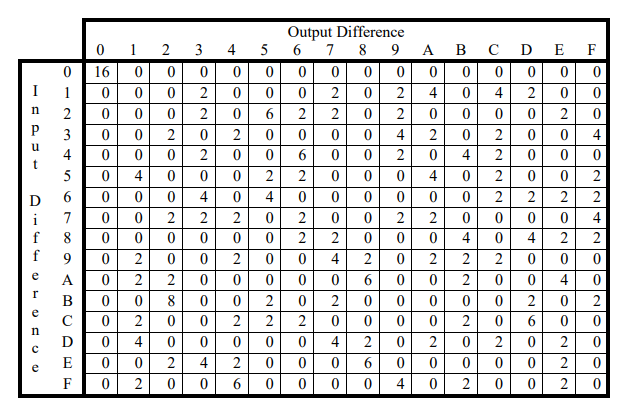
\includegraphics[scale=0.9]{Các công cụ và kĩ thuật sử dụng trong tấn công/diff distribution table.png}
    
    \caption{Bảng Phân phối Sai phân của S-box}
\end{figure}
\subsubsection{Phân tích Tính chất Vi phân của hệ mã hoàn chỉnh}
Ta sẽ sử dụng kiến trúc SPN (Substitution-Permutation Network) để mô phỏng việc Phân tích tính chất Vi phân này. Kiến trúc này được đề xuất bởi Feistel vào những năm 1973 và các toán tử cơ bản của nó tương tự với những gì tìm thấy ở DES hay rất nhiều hệ mã hiện đại khác, bao gồm cả Rijndael.

\begin{figure}[H]
    \centering
    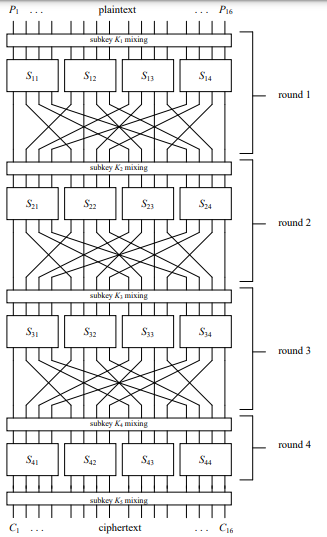
\includegraphics[scale=1.2]{Ảnh/triều/SPN.png}
    
    \caption{Kiến trúc SPN}
\end{figure}


Khi thông tin về tính chất Vi phân của các S-boxes trong SPN đã được tìm thấy, chúng ta có thể xác định tính chất Vi phân hữu dụng cho cả hệ. Điều này có thể thực hiện bằng cách ghép liên tiếp các cặp sai phân thích hợp. 

Xét tính chất Vi phân bao gồm $S_{12}, S_{23}, S_{32}, S_{33}.$ Đồ thị dưới đây biểu diễn ảnh hưởng của các cặp sai phân khi chúng di chuyển trên mạng, 
lưu ý tiến trình này xác định tính chất Vi phân của 3 vòng đầu tiên của hệ mã, không phải cả 4 vòng. Chúng ta sẽ thấy việc này hữu ích cho việc khôi phục bit từ khóa phụ cuối cùng ở phần sau. 
\begin{figure}[H]
    \centering
    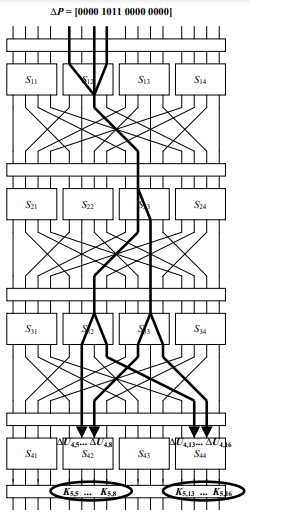
\includegraphics[scale=0.9]{Các công cụ và kĩ thuật sử dụng trong tấn công/spn1.png}
    
    \caption{Sample Differential Characteristics}
\end{figure}

Ta sử dụng cặp sai phân sau đây:

$S_{12}: \Delta X = B -> \Delta Y = 2$ với xác suất 8/16,

$S_{23}: \Delta X = 4 -> \Delta Y = 6$ với xác suất 6/16,

$S_{32}: \Delta X = 2 -> \Delta Y = 5$ với xác suất 6/16,

$S_{33}: \Delta X = 2 -> \Delta Y = 5$ với xác suất 6/16.

Sai phân đầu vào của hệ mã tương ứng với sai phân đầu vào tại vòng thứ nhất, được cho bởi:
$$ \Delta P = \Delta U_1 = [0000 1011 0000 0000]$$
Hệ quả là
$$ \Delta V_1 = [0000 0010 0000 0000]$$
và dựa vào cặp sai phân của $S_{12}$ ở trên và hoán vị ở vòng 1:
$$ \Delta U_2 = [0000 0000 0100 0000]$$ 
với xác suất 8/16 = 1/2 đối với sai phân đầu vào $\Delta P$. 

Tiếp theo vòng thứ 2, sử dụng cặp sai phân của $S_{23}$ ta có:
$$ \Delta V_2 = [0000 0000 0110 0000]$$
và hàm hoán vị ở vòng 2 cho ta:
$$ \Delta U_3 = [0000 0010 0010 0000]$$
với xác suất 6/16 đối với $\Delta U_2$ và xác suất 8/16 $\times$ 6/16 = 3/16 đối với $\Delta P$. 

Tương tự, ta sử dụng sai phân của S-box ở vòng thứ 3, $S_{23}$ và $S_{33}$, và hàm hoán vị ở vòng thứ 3 để thu được:
$$ \Delta V_3 = [0000 0101 0101 0000]$$ 
và 
$$ \Delta U_4 = [0000 0110 0000 0110]$$
với xác suất $(6/16)^2$ đối với $\Delta U_3$ và, do vậy, xác suất 8/16 $\times$ 6/16 $\times$ $(6/16)^2 = 27/1024$ đối với $\Delta P$.
\subsubsection{Trích xuất bit của khóa}
Một khi tính chất Vi phân của $R-1$ vòng của hệ mã $R$ vòng được khám phá với xác suất cao thích hợp, ta có thể tấn công hệ mã bằng cách khôi phục bit từ khóa phụ cuối cùng mà trong ví dụ của chúng ta, chính là việc khôi phục bit từ khóa phụ $K_5$. 

Quá trình mã hóa 1 phần được thực hiện với từng cặp bản rõ tương ứng với sai phân đầu vào $\Delta P$ cho tất cả các giá trị có thể của bộ phận khóa mục tiêu để đếm số lần trùng giữa sai phân đầu vào và sai phân đầu ra tương ứng.

Dưới đây là bảng mô phỏng tấn công bằng cách sinh 5000 bản rõ-mã chọn trước. Bộ phận khóa mục tiêu chính xác là $[K_{5,5}...K_{5,8}, K_{5,13}...K_{5,16}] = [0010,0100] = [2,4]_{hex}$. Như kỳ vọng, số lần trùng quan sát được lớn nhất là của bộ phận khóa $[2,4]_{hex},$ chứng tỏ cuộc tấn công đã thành công khôi phục bit của khóa phụ. Bảng dưới đây tổng hợp một phần dữ liệu từ việc phân tích các khóa phụ (Bảng hoàn thiện chứa 256 phần tử tương ứng 256 giá trị có thể của bộ phận khóa mục tiêu). Giá trị trong bảng thể hiện xấp xỉ xác suất xuất hiện của các cặp đúng đối với ứng viên khóa bộ phận.

\begin{figure}[H]
    \centering
    \includegraphics[scale=0.9]{Các công cụ và kĩ thuật sử dụng trong tấn công/experimential results diff.png}
    
    \caption{Kết quả Tấn công Vi phân thực nghiệm}
\end{figure}










\newpage
\subsection{Tấn công Tuyến tính (Linear Cryptanalysis) }
Các kết quả của phần này được trích từ \cite{hey2002}.
\subsubsection{Nguyên lý cơ bản}
Được đề xuất bởi Mitsuru Matsui trong cuốn "Advance in Cryptology" năm 1993, ông chứng minh Tấn công Tuyến tính có thể phá mã DES với $2^{47}$ bản rõ. Một năm sau, ông cải tiến kỹ thuật của mình và chứng minh chỉ cần $2^{43}$ bản rõ. Cho đến ngày nay, phương pháp tấn công Tuyến tính vẫn là phương pháp tấn công nhanh nhất để tấn công DES.

Tấn công Tuyến tính khai thác sự xuất hiện với xác suất cao của 1 biểu diễn tuyến tính nào đó giữa các bit của bản rõ và các bit của bản mã. Đây là dạng tấn công biết trước bản rõ, có nghĩa là kẻ tấn công được giả thiết có thông tin về 1 tập bản rõ và bản mã tương ứng nhất định. Trong nhiều ứng dụng và ngữ cảnh, có thể giả sử kẻ tấn công có thông tin về 1 tập ngẫu nhiên bản rõ và bản mã tương ứng.

Ý tưởng cơ bản của Tấn công tuyến tính là tìm kiếm một biểu diễn tuyến tính với xác suất đúng cao hơn ngẫu nhiên của các bit bản rõ, các bit bản mã, và các bit của khóa, cụ thể có dạng:
$$ X_{i_1} \oplus X_{i_2} \oplus ... \oplus X_{i_u} \oplus Y_{j_1} \oplus Y_{j_2} \oplus ... \oplus Y_{j_v} = K_{k_1} \oplus K_{k_2} \oplus ... \oplus K_{k_w} $$ 
hoặc dạng tương đương 
$$X_{i_1} \oplus X_{i_2} \oplus ... \oplus X_{i_u} \oplus Y_{j_1} \oplus Y_{j_2} \oplus ... \oplus Y_{j_v} = 0 $$
Trong đó $X_i$ là bit thứ $i$ của $X$, $Y_j$ là bit thứ $j$ của $Y$, $\oplus$ ký hiệu cho phép toán XOR.

Giả sử $p_L$ là xác suất biểu diễn trên đúng khi chọn ngẫu nhiên bản rõ và bản mã tương ứng, ta định nghĩa độ lệch (\emph{bias}) tương ứng là $p_L - 1/2.$ Độ lớn của \emph{bias} càng lớn, chứng tỏ độ ngẫu nhiên của hệ mật càng yếu, khả năng tấn công Tuyến tính với ít bản rõ cho trước càng cao.

Trước khi đi vào phân tích tính chất tuyến tính của 1 hệ mã cụ thể ta giới thiệu 1 công cụ hỗ trợ cho việc tính toán \emph{bias} một cách đơn giản hơn:

\textbf{(Piling-up Lemma)} Cho $n$ biến ngẫu nhiên độc lập toàn thể $X_1, X_2,..., X_n$. Khi đó:
    $$P(X_1 \oplus X_2 \oplus ... \oplus X_n = 0) = \frac{1}{2} + 2^{n-1} \prod_{i=1}^n \epsilon_i,  $$
    trong đó $\epsilon_i$ là độ lệch (\emph{bias}) của $X_i$.
\subsubsection{Phân tích tính chất Tuyến tính của S-box}
Ta vẫn sử dụng S-box giống như ở phần trước:
Ta sẽ phân tích tính chất Vi phân của S-box sau:
\begin{figure}[H]
    \centering
    \includegraphics[scale=0.9]{Các công cụ và kĩ thuật sử dụng trong tấn công/S-boz.png}
\end{figure}
Ví dụ, xét biểu diễn tuyến tính $X_2 \oplus X_3 \oplus Y_1 \oplus Y_3 \oplus Y_4 = 0$ hay một cách tương đương $ X_2 \oplus  X_3 = Y_1 \oplus Y_3 \oplus Y_4.$ Kiểm tra tất cả 16 giá trị có thể của $X$ và đối chiếu với đầu ra tương ứng của $Y$, ta quan sát được biểu thức đúng với 12 trên 16 trường hợp. Như vậy giá trị \emph{bias} trong trường hợp này là $\frac{12}{16}-\frac{1}{2} = \frac{1}{4}.$ Tương tự ta có thể tính toán, với phương trình $X_1 \oplus X_4 = Y_2$ có giá trị \emph{bias} là 0 và phương trình $X_3 \oplus X_4 = Y_1 \oplus Y_4$ có độ \emph{bias} là $\frac{-3}{8}.$
Khả năng thành công của tấn công, như chúng ta sẽ thấy, phụ thuộc vào độ lớn của giá trị \emph{bias} này.

Ta có bảng phân tích một số biểu diễn xấp xỉ tuyến tính  của S-box:
 \begin{figure}
    \centering
    \includegraphics[scale = 0.9]{Các công cụ và kĩ thuật sử dụng trong tấn công/sample linear sbox.png}
    \caption{Phân tích một số biểu diễn xấp xỉ tuyến tính S-box}
    
    \end{figure}

    Kết quả tính toán cụ thể tất cả các xấp xỉ tuyến tính của S-box có thể cho bởi bảng Xấp xỉ Tuyến tính dưới đây. Mỗi phần tử trong bảng biểu diễn số lần trùng nhau giữa giá trị của phương trình tuyến tính của tổng các bit đầu vào và phương trình tuyến tính tổng các bit đầu ra (dưới dạng thập lục phân) trừ đi 8. Ví dụ, \emph{bias} của phương trình $X_3 \oplus X_4 = Y_1 \oplus Y_4$ (tương ứng với đầu vào hệ thập lục phân 3 và đầu ra 9) là $\frac{-6}{16} = \frac{-3}{8}$ và xác suất phương trình nhận giá trị đúng là $\frac{1}{2} - \frac{3}{8} = \frac{1}{8}$.
    \begin{figure}
    \centering
    \includegraphics[scale = 0.9]{Các công cụ và kĩ thuật sử dụng trong tấn công/linear approx table.png}
    \caption{Bảng xấp xỉ tuyến tính S-box}
    
    \end{figure}
\subsubsection{Phân tích tính chất Tuyến tính của hệ mã hoàn chỉnh}
Tương tự như phần về Tấn công Vi phân, khi đã có thông tin về xấp xỉ tuyến tính của tất cả S-box trong SPN, chúng ta có thể xác định xấp xỉ tuyến tính cho cả hệ mã. Điều này có thể thực hiện bằng cách ghép liên tiếp các xấp xỉ tuyến tính thích hợp. Ta sẽ đưa ra ví dụ dưới đây:

Xét xấp xỉ tuyến tính bao gồm $S_{12}, S_{22}, S_{32}, S_{34}$ như hình dưới. Lưu ý rằng quá trình này đưa ra 1 biểu diễn xấp xỉ cho 3 vòng đầu của hệ mã chứ không phải cả 4 vòng. Ta sẽ thấy ở phần sau từ điều này có thể khôi phục lại 1 phần bit của khóa phụ cuối cùng.

\begin{figure}
    \centering
    \includegraphics[scale = 1.5]{Các công cụ và kĩ thuật sử dụng trong tấn công/sample linear app.png}
    
    \caption{Sample Linear Approximation}
    \end{figure}

Ta xét các xấp xỉ sau của S-box:
$$S_{12}: X_1 \oplus X_3 \oplus X_4 = Y_2$$ với xác suất 12/16 và bias +1/4,
$$ S_{22}: X_2 = Y_2 \oplus Y_4$$ với xác suất 4/16 và bias -1/4,
$$ S_{32}: X_2 = Y_2 \oplus Y_4$$ với xác suất 4/16 và bias -1/4, 
$$ S_{34} = X_2 \oplus Y_4$$ với xác suất 4/16 và bias -1/4.

Gọi $U_i(V_i)$ thể hiện khối 16 bit đầu vào (đầu ra) tại vòng thứ $i$ của S-box và $U_{i,j} (V_{i,j})$ thể hiện bit thứ $j$ của khối $U_i (V_i)$. Tương tự, gọi $K_i$ là khối khóa phụ tại vòng thứ $i$.

Ta có  $U_1 = P \oplus K_1$, sử dụng xấp xỉ tuyến tính ở vòng thứ nhất, ta có:
$$ V_{1,6} = U_{1,5} \oplus U_{1,7} \oplus U_{1,8} = (P_5 \oplus K_{1,5}) \oplus (P_7 \oplus K_{1,7}) \oplus (P_8 \oplus K_{1,8})$$
với xác suất 3/4. Với xấp xỉ ở vòng thứ 2, ta có:
$$ V_{2,6} \oplus V_{2,8} = U_{2,6}$$
với xác suất 1/4. Từ $U_{2,6} = V_{1,6} \oplus K_{2,6}$, ta thu được xấp xỉ dưới dạng 
$$ V_{2,6} \oplus V_{2,8} = V_{1,6} \oplus K_{2,6}$$ với xác suất 1/4 và từ đó ta có :
$$ V_{2,6} \oplus V_{2,8} \oplus P_5 \oplus P_7 \oplus P_8 \oplus K_{1,5} \oplus K_{1,7} \oplus K_{1,8} \oplus K_{2,6} = 0$$
với xác suất 1/2 + 2(3/4-1/2)(1/4-1/2) = 3/8 theo Bổ đề Pilling Up.

Ở vòng 3, ta có 
$$ V_{3,6} \oplus V_{3,8} = U_{3,6}  $$ 
với xác suất 1/4 và 
$$ V_{3,14} \oplus V_{3,16} = U_{3,14}$$
với xác suất 1/4. Do đó, từ $U_{3,6} = V_{2,6} \oplus K_{3,6}$ và $U_{3,14} = V_{2,8} \oplus K_{3,14}$ ta có:
$$V_{3,6} \oplus V_{3,8} \oplus V_{3,14} \oplus V_{3,16} \oplus V_{2,6} \oplus K_{3,6} \oplus V_{2,8} \oplus K_{3,14} = 0$$
với xác suất $1/2 + 2(1/4-1/2)^2 = 5/8$.

Từ đó ta có:
$$ V_{3,6} \oplus V_{3,8} \oplus V_{3,14} \oplus V_{3,16} \oplus P_5 \oplus P_7 \oplus P_8 \oplus K_{1,5} \oplus K_{1,7} \oplus K_{1,8} \oplus K_{2,6} \oplus K_{3,6} \oplus K_{3,14} = 0.$$

Chú ý rằng $U_{4,6} = V_{3,6} \oplus K_{4,6}$, $U_{4,8} = V_{3,14} \oplus K_{4,8},$ $U_{4,14} = V_{3,8} \oplus K_{4,14}$ và $U_{4,16} = V_{3,16} \oplus K_{4,16},$ ta có thể viết lại như sau: 
$$ U_{4,6} \oplus U_{4,8} \oplus U_{4,14} \oplus U_{4,16} \oplus P_5 \oplus P_7 \oplus P_8 \oplus \small{\sum_{K}} = 0$$ \\
với
$\sum_{K} = K_{1,5} \oplus K_{1,7} \oplus K_{1,8} \oplus K_{2,6} \oplus K_{3,6} \oplus K_{3,14} \oplus K_{4,6} \oplus K_{4,8} \oplus K_{4,14} \oplus K_{4,16}$
và $\sum_K$ cố định bằng 0 hoặc 1 tùy vào khóa của hệ mã. Theo bổ đề Pilling Up, biểu thức trên đúng với xác suất 15/32 (và bias -1/32).
Như vậy biểu thức
 $$ U_{4,6} \oplus U_{4,8} \oplus U_{4,14} \oplus U_{4,16} \oplus P_5 \oplus P_7 \oplus P_8 = 0$$ 
 đúng với xác suất 15/32 hoặc 17/32. Nói cách khác, ta có 1 xấp xỉ tuyến tính cho 3 vòng đầu của cipher với độ lớn bias 1/32. Phần tiếp theo ta sử dụng điều này để khôi phục bit từ khóa.
 \subsubsection{Khôi phục bit từ khóa}
Giống như phần Tấn công Tuyến tính, ta có thể trích ra 1 phần bit của khóa $K_5$ sau 3 vòng Xấp xỉ tuyến tính. Quy trình bao gồm với mọi giá trị có thể của khóa bộ phận mục tiêu, bit của bản mã tương ứng được XOR với bit của khóa bộ phận mục tiêu và kết quả được chạy ngược lại qua S-box tương ứng. Điều này được thực hiện với tất cả cặp bản rõ, bản mã đã biết và 1 biến đếm được sử dụng với mỗi khóa bộ phận mục tiêu. Biến đếm này tăng mỗi lần biểu diễn tuyến tính đúng với bit ở vòng cuối của S-box và bản rõ đã biết. Khóa bộ phận mục tiêu có biến đếm lệch lớn nhất so với 1 nửa độ lớn không gian bản rõ - bản mã được cho là khóa bộ phận chính xác.

Dưới đây là bảng mô phỏng tấn công với 10000 bản rõ - bản mã biết trước đối với 2 khóa bộ phận mục tiêu $[K_{5,5}...K_{5,8}] = [0010]$ (hex 2) và $[K_{5,13}...K_{5,16} = [0100]$ (hex 4). Như đã dự đoán, $[2,4]_{hex}$ có biến đếm lệch nhiều nhất so với 5000, và trong thực tế, cũng là khóa bộ phận thực sự của khóa gốc ban đầu.
    \begin{figure}
    \centering
    \includegraphics[scale = 0.9]{Các công cụ và kĩ thuật sử dụng trong tấn công/exp linear.png}
    
    \caption{Kết quả thực nghiệm Tấn công Tuyến tính}
    \end{figure}
    
\section{Xây dựng Chương trình Mô phỏng }
Sau khi tìm hiểu về các phương pháp mã hoá và tấn công hệ mật khoá đối xứng, bọn em thực hiện xây dựng chương trình thực hiện thuật toán DES, AES và phương pháp tấn công Brute Force bằng ngôn ngữ C++:
\subsection{DES (Data Encryption Standard)}
\subsubsection{Hàm tạo khoá vòng}
\begin{minted}[mathescape,
	numbersep=5pt,
	frame=lines,
	framesep=2mm,
	breaklines,
	baselinestretch=1.2,
	bgcolor=LightGray,
	fontsize=\footnotesize,
	linenos]{C++}
	void generate_keys(string key) {
		int PC_1[56] = {
			57,49,41,33,25,17,9, 
			1,58,50,42,34,26,18, 
			10,2,59,51,43,35,27, 
			19,11,3,60,52,44,36,		 
			63,55,47,39,31,23,15, 
			7,62,54,46,38,30,22, 
			14,6,61,53,45,37,29, 
			21,13,5,28,20,12,4 
		};
		
		int PC_2[48] = {
			14,17,11,24,1,5, 
			3,28,15,6,21,10, 
			23,19,12,4,26,8, 
			16,7,27,20,13,2, 
			41,52,31,37,47,55, 
			30,40,51,45,33,48, 
			44,49,39,56,34,53, 
			46,42,50,36,29,32 
		};
		
		// Hoán vị key theo bảng pc_1
		string perm_key = "";
		for(int i = 0; i < 56; i++) {
			perm_key += key[PC_1[i] - 1];
		}
		
		// Xác định giá trị C0 và D0
		string C = perm_key.substr(0, 28);
		string D = perm_key.substr(28, 28);
		
		for(int i = 0; i < 16; i++) {
			// Lần lặp thứ 1, 2, 9, 16 dịch trái 1 lần; những vị trí còn lại dịch trái 2 lần
			if (i == 0 || i == 1 || i == 8 || i == 15) {
				C = shift_left_once(C);
				D = shift_left_once(D);
			} else {
				C = shift_left_twice(C);
				D = shift_left_twice(D);
			}
			
			string combined_key = C + D;
			
			string round_key = "";
			for(int j = 0; j < 48; j++) {
				round_key += combined_key[PC_2[j] - 1];
			}
			round_keys[i] = round_key; 
		}
	}
\end{minted}
\subsubsection{Hàm tính \(f(R, K)\)}
\begin{minted}[mathescape,
	numbersep=5pt,
	frame=lines,
	framesep=2mm,
	breaklines,
	baselinestretch=1.2,
	bgcolor=LightGray,
	fontsize=\footnotesize,
	linenos]{C++}
	string f(string R, string round_key) {
		int E[48] = {
			32,1,2,3,4,5,4,5, 
			6,7,8,9,8,9,10,11, 
			12,13,12,13,14,15,16,17, 
			16,17,18,19,20,21,20,21, 
			22,23,24,25,24,25,26,27, 
			28,29,28,29,30,31,32,1
		};
		
		// Hàm S-box
		int S[8][4][16] = 
		{{ 
				14,4,13,1,2,15,11,8,3,10,6,12,5,9,0,7, 
				0,15,7,4,14,2,13,1,10,6,12,11,9,5,3,8, 
				4,1,14,8,13,6,2,11,15,12,9,7,3,10,5,0, 
				15,12,8,2,4,9,1,7,5,11,3,14,10,0,6,13 
			}, 
			{ 
				15,1,8,14,6,11,3,4,9,7,2,13,12,0,5,10, 
				3,13,4,7,15,2,8,14,12,0,1,10,6,9,11,5, 
				0,14,7,11,10,4,13,1,5,8,12,6,9,3,2,15, 
				13,8,10,1,3,15,4,2,11,6,7,12,0,5,14,9 
			}, 
			{ 
				10,0,9,14,6,3,15,5,1,13,12,7,11,4,2,8, 
				13,7,0,9,3,4,6,10,2,8,5,14,12,11,15,1, 
				13,6,4,9,8,15,3,0,11,1,2,12,5,10,14,7, 
				1,10,13,0,6,9,8,7,4,15,14,3,11,5,2,12 
			}, 
			{ 
				7,13,14,3,0,6,9,10,1,2,8,5,11,12,4,15, 
				13,8,11,5,6,15,0,3,4,7,2,12,1,10,14,9, 
				10,6,9,0,12,11,7,13,15,1,3,14,5,2,8,4, 
				3,15,0,6,10,1,13,8,9,4,5,11,12,7,2,14 
			}, 
			{ 
				2,12,4,1,7,10,11,6,8,5,3,15,13,0,14,9, 
				14,11,2,12,4,7,13,1,5,0,15,10,3,9,8,6, 
				4,2,1,11,10,13,7,8,15,9,12,5,6,3,0,14, 
				11,8,12,7,1,14,2,13,6,15,0,9,10,4,5,3 
			}, 
			{ 
				12,1,10,15,9,2,6,8,0,13,3,4,14,7,5,11, 
				10,15,4,2,7,12,9,5,6,1,13,14,0,11,3,8, 
				9,14,15,5,2,8,12,3,7,0,4,10,1,13,11,6, 
				4,3,2,12,9,5,15,10,11,14,1,7,6,0,8,13 
			}, 
			{ 
				4,11,2,14,15,0,8,13,3,12,9,7,5,10,6,1, 
				13,0,11,7,4,9,1,10,14,3,5,12,2,15,8,6, 
				1,4,11,13,12,3,7,14,10,15,6,8,0,5,9,2, 
				6,11,13,8,1,4,10,7,9,5,0,15,14,2,3,12 
			}, 
			{ 
				13,2,8,4,6,15,11,1,10,9,3,14,5,0,12,7, 
				1,15,13,8,10,3,7,4,12,5,6,11,0,14,9,2, 
				7,11,4,1,9,12,14,2,0,6,10,13,15,3,5,8, 
				2,1,14,7,4,10,8,13,15,12,9,0,3,5,6,11 
		}};
		
		int P[32] = { 
			16,7,20,21,29,12,28,17, 
			1,15,23,26,5,18,31,10, 
			2,8,24,14,32,27,3,9,
			19,13,30,6,22,11,4,25 
		}; 
		
		// Hoán vị R
		string RE = "";
		for(int i = 0; i < 48; i++) {
			RE += R[E[i] - 1];
		}
		
		string xored = XOR(RE, round_key);
		string res = "";
		for(int i = 0; i < 8; i++) {
			string row_bin = xored.substr(i * 6, 1) + xored.substr(i * 6 + 5, 1);
			int row = convertBintoDec(row_bin);
			string col_bin = xored.substr(i * 6 + 1, 1) + xored.substr(i * 6 + 2, 1) + xored.substr(i * 6 + 3, 1) + xored.substr(i * 6 + 4, 1);
			int col = convertBintoDec(col_bin);
			
			int val = S[i][row][col];
			res += convertDectoBin(val);
		}
		
		string f = "";
		for(int i = 0; i < 32; i++) {
			f += res[P[i] - 1];
		}
		return f;
	}
\end{minted}

\subsubsection{Hàm DES}
\begin{minted}[mathescape,
	numbersep=5pt,
	frame=lines,
	framesep=2mm,
	breaklines,
	baselinestretch=1.2,
	bgcolor=LightGray,
	fontsize=\footnotesize,
	linenos]{C++}
	string DES(string plain_text) {
		int IP[64] = {
			58,50,42,34,26,18,10,2, 
			60,52,44,36,28,20,12,4, 
			62,54,46,38,30,22,14,6, 
			64,56,48,40,32,24,16,8, 
			57,49,41,33,25,17,9,1, 
			59,51,43,35,27,19,11,3, 
			61,53,45,37,29,21,13,5, 
			63,55,47,39,31,23,15,7
		};
		
		int inverse_IP[64] = {
			40,8,48,16,56,24,64,32, 
			39,7,47,15,55,23,63,31, 
			38,6,46,14,54,22,62,30, 
			37,5,45,13,53,21,61,29, 
			36,4,44,12,52,20,60,28, 
			35,3,43,11,51,19,59,27, 
			34,2,42,10,50,18,58,26, 
			33,1,41,9,49,17,57,25 
		};
		
		int E[48] = {
			32,1,2,3,4,5,4,5, 
			6,7,8,9,8,9,10,11, 
			12,13,12,13,14,15,16,17, 
			16,17,18,19,20,21,20,21, 
			22,23,24,25,24,25,26,27, 
			28,29,28,29,30,31,32,1
		};
		
		
		// Thực hiện hoán vị bản rõ
		string permutation = "";
		for(int i = 0; i < 64; i++) {
			permutation += plain_text[IP[i] - 1];
		}
		
		string L = permutation.substr(0, 32);
		string R = permutation.substr(32, 32);
		
		for(int i = 0; i < 16; i++) {
			string xored1 = XOR(L, f(R, round_keys[i]));
			L = xored1;
			if (i < 15) {
				string temp = R;
				R = xored1;
				L = temp;
			}
		}
		
		string combined_text = L + R;
		string ciphertext =""; 
		// Áp dụng bảng hoán vị IP-1
		for(int i = 0; i < 64; i++){ 
			ciphertext += combined_text[inverse_IP[i] - 1]; 
		}
		
		return ciphertext;
	}
\end{minted}

\subsubsection{Hàm encrypt}
\begin{minted}[mathescape,
	numbersep=5pt,
	frame=lines,
	framesep=2mm,
	breaklines,
	baselinestretch=1.2,
	bgcolor=LightGray,
	fontsize=\footnotesize,
	linenos]{C++}
	void encrypt() {
		string plain_text;
		string key;
		system("cls");
		cout << "Nhap ban ro (16 ki tu): ";
		do {
			cin >> plain_text;
			if (!is_valid(plain_text, 16))
			cout << "Moi ban nhap lai ban ro : ";
		} while (!is_valid(plain_text, 16));
		
		cout << "Nhap khoa (16 ki tu): ";
		do {
			cin >> key;
			if (!is_valid(key, 16))
			cout << "Moi ban nhap lai ban ro : ";
		} while (!is_valid(key, 16));
		
		generate_keys(convertHextoBin(key));
		
		string ciphertext = DES(convertHextoBin(plain_text));
		cout <<  "Ban ro: " << plain_text << endl;
		cout << "Ban ma: " << convertBintoHex(ciphertext) << endl;
	}
\end{minted}
\subsubsection{Hàm decrypt}
Hàm decrypt được thực hiện tương tự encrypt tuy nhiên, mảng khoá vòng được đảo chiều lại.
\begin{minted}[mathescape,
	numbersep=5pt,
	frame=lines,
	framesep=2mm,
	breaklines,
	baselinestretch=1.2,
	bgcolor=LightGray,
	fontsize=\footnotesize,
	linenos]{C++}
	void decrypt() {
		string ciphertext;
		string key;
		system("cls");
		
		cout << "Nhap ban ma (16 ki tu): ";
		do {
			cin >> ciphertext;
			if (!is_valid(ciphertext, 16))
			cout << "Moi ban nhap lai ban ro : ";
		} while (!is_valid(ciphertext, 16));
		
		cout << "Nhap khoa (16 ki tu): ";
		do {
			cin >> key;
			if (!is_valid(key, 16))
			cout << "Moi ban nhap lai ban ro : ";
		} while (!is_valid(key, 16));
		
		
		generate_keys(convertHextoBin(key));
		
		
		int i = 15;
		int j = 0;
		while(i > j)
		{
			string temp = round_keys[i];
			round_keys[i] = round_keys[j];
			round_keys[j] = temp;
			i--;
			j++;
		}
		
		string plaintext = DES(convertHextoBin(ciphertext));
		cout << "Ban ma: " << ciphertext << endl;
		cout << "Ban ro: " << convertBintoHex(plaintext) << endl;
	} 
\end{minted}
\subsection{AES (Advanced Encryption Standard)}
\subsubsection{Các hàm phụ}
\begin{minted}[mathescape,
	numbersep=5pt,
	frame=lines,
	framesep=2mm,
	breaklines,
	baselinestretch=1.2,
	bgcolor=LightGray,
	fontsize=\footnotesize,
	linenos]{C++}
	unsigned int RotWord(unsigned int w)
	{
		//Dich vong trai 1 byte
		unsigned int byte1 = (w >> 24) & 0xff;
		unsigned int byte234 = w & 0xffffff;
		unsigned int rot = (byte234 << 8) | byte1;
		return rot;
	}
	
	unsigned int SubWord(unsigned int w)
	{
		int S[] = {0x63, 0x7C, 0x77, 0x7B, 0xF2, 0x6B, 0x6F, 0xC5, 0x30, 0x01, 0x67, 0x2B, 0xFE, 0xD7, 0xAB, 0x76, 
			0xCA, 0x82, 0xC9, 0x7D, 0xFA, 0x59, 0x47, 0xF0, 0xAD, 0xD4, 0xA2, 0xAF, 0x9C, 0xA4, 0x72, 0xC0, 
			0xB7, 0xFD, 0x93, 0x26, 0x36, 0x3F, 0xF7, 0xCC, 0x34, 0xA5, 0xE5, 0xF1, 0x71, 0xD8, 0x31, 0x15, 
			0x04, 0xC7, 0x23, 0xC3, 0x18, 0x96, 0x05, 0x9A, 0x07, 0x12, 0x80, 0xE2, 0xEB, 0x27, 0xB2, 0x75, 
			0x09, 0x83, 0x2C, 0x1A, 0x1B, 0x6E, 0x5A, 0xA0, 0x52, 0x3B, 0xD6, 0xB3, 0x29, 0xE3, 0x2F, 0x84, 
			0x53, 0xD1, 0x00, 0xED, 0x20, 0xFC, 0xB1, 0x5B, 0x6A, 0xCB, 0xBE, 0x39, 0x4A, 0x4C, 0x58, 0xCF, 
			0xD0, 0xEF, 0xAA, 0xFB, 0x43, 0x4D, 0x33, 0x85, 0x45, 0xF9, 0x02, 0x7F, 0x50, 0x3C, 0x9F, 0xA8, 
			0x51, 0xA3, 0x40, 0x8F, 0x92, 0x9D, 0x38, 0xF5, 0xBC, 0xB6, 0xDA, 0x21, 0x10, 0xFF, 0xF3, 0xD2, 
			0xCD, 0x0C, 0x13, 0xEC, 0x5F, 0x97, 0x44, 0x17, 0xC4, 0xA7, 0x7E, 0x3D, 0x64, 0x5D, 0x19, 0x73, 
			0x60, 0x81, 0x4F, 0xDC, 0x22, 0x2A, 0x90, 0x88, 0x46, 0xEE, 0xB8, 0x14, 0xDE, 0x5E, 0x0B, 0xDB, 
			0xE0, 0x32, 0x3A, 0x0A, 0x49, 0x06, 0x24, 0x5C, 0xC2, 0xD3, 0xAC, 0x62, 0x91, 0x95, 0xE4, 0x79, 
			0xE7, 0xC8, 0x37, 0x6D, 0x8D, 0xD5, 0x4E, 0xA9, 0x6C, 0x56, 0xF4, 0xEA, 0x65, 0x7A, 0xAE, 0x08, 
			0xBA, 0x78, 0x25, 0x2E, 0x1C, 0xA6, 0xB4, 0xC6, 0xE8, 0xDD, 0x74, 0x1F, 0x4B, 0xBD, 0x8B, 0x8A, 
			0x70, 0x3E, 0xB5, 0x66, 0x48, 0x03, 0xF6, 0x0E, 0x61, 0x35, 0x57, 0xB9, 0x86, 0xC1, 0x1D, 0x9E, 
			0xE1, 0xF8, 0x98, 0x11, 0x69, 0xD9, 0x8E, 0x94, 0x9B, 0x1E, 0x87, 0xE9, 0xCE, 0x55, 0x28, 0xDF, 
			0x8C, 0xA1, 0x89, 0x0D, 0xBF, 0xE6, 0x42, 0x68, 0x41, 0x99, 0x2D, 0x0F, 0xB0, 0x54, 0xBB, 0x16
		};
		unsigned int kq = 0;
		for(int i = 1; i <= 4; i++)	
		{
			unsigned int bytei = (w >> (32 - i*8)) & 0xff;
			unsigned int subB = S[bytei];
			kq = (kq << 8) | subB;
		}
		//printf("\n\tSubWord(%X) = ",w); ShowWord(kq);
		return kq;
	}
	
	unsigned int XorRcon(unsigned int w, int j)
	{     
		int Rc[] = {
			0x8d, 0x01, 0x02, 0x04, 0x08, 0x10, 0x20, 0x40, 0x80, 0x1b, 0x36, 0x6c, 0xd8, 0xab, 0x4d, 0x9a,
			0x2f, 0x5e, 0xbc, 0x63, 0xc6, 0x97, 0x35, 0x6a, 0xd4, 0xb3, 0x7d, 0xfa, 0xef, 0xc5, 0x91, 0x39
		};
		unsigned int byte1 = (w >> 24) & 0xff;
		unsigned int kqXor = (byte1 ^ Rc[j]) & 0xff;
		unsigned int byte234 = w & 0xffffff;
		unsigned int kq = (kqXor << 24) | byte234;
		
		return kq;
	}
	
	unsigned int Trans(unsigned int w, int j)
	{
		unsigned int rotW = RotWord(w);
		unsigned int subW = SubWord(rotW);
		unsigned int kq = XorRcon(subW, j);
		return kq;
	}
	
	unsigned int* KeyExpansion(unsigned int Key[4])
	{
		unsigned int *w = new unsigned int[44];
		w[0] = Key[0]; 	
		w[1] = Key[1]; 	
		w[2] = Key[2]; 	
		w[3] = Key[3];
		for(int i = 4; i < 44; i++)
		{
			if(i % 4 == 0) w[i] = Trans(w[i - 1], i/4) ^ w[i - 4];
			else w[i] = w[i - 1] ^ w[i - 4];
		}
		return w;
	}
\end{minted}
\subsubsection{Mã hoá}
\begin{enumerate}
	\item Hàm AddRoundKey()
	\begin{minted}[mathescape,
		numbersep=5pt,
		frame=lines,
		framesep=2mm,
		breaklines,
		baselinestretch=1.2,
		bgcolor=LightGray,
		fontsize=\footnotesize,
		linenos]{C++}
		unsigned int* AddRoundKey(unsigned int state[4], unsigned int *K)
		{
			unsigned int *kq = new unsigned int[4];
			kq[0] = state[0] ^ K[0];
			kq[1] = state[1] ^ K[1];
			kq[2] = state[2] ^ K[2];
			kq[3] = state[3] ^ K[3];
			
			return kq;
		}
	\end{minted}
	\item Hàm SubBytes()
	\begin{minted}[mathescape,
		numbersep=5pt,
		frame=lines,
		framesep=2mm,
		breaklines,
		baselinestretch=1.2,
		bgcolor=LightGray,
		fontsize=\footnotesize,
		linenos]{C++}
		unsigned int* SubBytes(unsigned int state[4])
		{
			unsigned int *kq = new unsigned int[4];
			for (int i = 0; i < 4; i++){
				kq[i] = SubWord(state[i]);
			}
			
			return kq;
		}
	\end{minted}
	\item Hàm ShiftRows()
	\begin{minted}[mathescape,
		numbersep=5pt,
		frame=lines,
		framesep=2mm,
		breaklines,
		baselinestretch=1.2,
		bgcolor=LightGray,
		fontsize=\footnotesize,
		linenos]{C++}
		unsigned int* ShiftRows(unsigned int state[4])
		{
			unsigned int *kq = new unsigned int[4];
			for (int i = 0; i < 4; i++)
			{
				unsigned int byte1 = state[i] & 0xff000000;
				unsigned int byte2 = state[(i + 1) % 4] & 0xff0000;
				unsigned int byte3 = state[(i + 2) % 4] & 0xff00;
				unsigned int byte4 = state[(i + 3) % 4] & 0xff;
				
				kq[i] = byte1 | byte2 | byte3 | byte4;
			}
			return kq;
		}
	\end{minted}
	\item Hàm MixColumns()
	\begin{minted}[mathescape,
		numbersep=5pt,
		frame=lines,
		framesep=2mm,
		breaklines,
		baselinestretch=1.2,
		bgcolor=LightGray,
		fontsize=\footnotesize,
		linenos]{C++}
		unsigned int Nhan2(unsigned int w)
		{
			unsigned int kq = w << 1;
			if(kq > 256) kq = kq ^ 0x11b;
			kq = kq & 0xFF;
			return kq;
		}
		
		unsigned int Nhan3(unsigned int w)
		{
			unsigned int kq = w ^ Nhan2(w);
			kq = kq & 0xFF;
			return kq;
		}
		
		unsigned int NhanCot(unsigned int w)
		{
			unsigned int kq;
			unsigned int byte1 = (w >> 24) & 0xFF;
			unsigned int byte2 = (w >> 16) & 0xFF;
			unsigned int byte3 = (w >> 8) & 0xFF;
			unsigned int byte4 = w & 0xFF;
			unsigned int kq1 = Nhan2(byte1) ^ Nhan3(byte2) ^ byte3 ^ byte4;
			unsigned int kq2 = byte1 ^ Nhan2(byte2) ^ Nhan3(byte3) ^ byte4;
			unsigned int kq3 = byte1 ^ byte2 ^ Nhan2(byte3) ^ Nhan3(byte4);
			unsigned int kq4 = Nhan3(byte1) ^ byte2 ^ byte3 ^ Nhan2(byte4);
			kq = (kq1 << 24) | (kq2 << 16) | (kq3 << 8) | kq4;
			//cout << "\n\t"; ShowWord(kq);
			return kq;
		}
		unsigned int* MixColumns(unsigned int state[4])
		{
			unsigned int *kq = new unsigned int[4];
			for (int i = 0; i < 4; i++) kq[i] = NhanCot(state[i]);
			
			return kq;
		}
	\end{minted}
\end{enumerate}

\subsubsection{Giải mã}
\begin{enumerate}
	\item Hàm InvSubBytes()
	\begin{minted}[mathescape,
		numbersep=5pt,
		frame=lines,
		framesep=2mm,
		breaklines,
		baselinestretch=1.2,
		bgcolor=LightGray,
		fontsize=\footnotesize,
		linenos]{C++}
		unsigned int* InvSubBytes(unsigned int state[4])
		{
			unsigned int *kq = new unsigned int[4];
			for (int i = 0; i < 4; i++) kq[i] = InvSubWord(state[i]);
			return kq;
		}
	\end{minted}
	\item Hàm InvShiftRows()
	\begin{minted}[mathescape,
		numbersep=5pt,
		frame=lines,
		framesep=2mm,
		breaklines,
		baselinestretch=1.2,
		bgcolor=LightGray,
		fontsize=\footnotesize,
		linenos]{C++}
		unsigned int* InvShiftRows(unsigned int state[4])
		{
			unsigned int *kq = new unsigned int[4];
			for (int i = 0; i < 4; i++)
			{
				unsigned int byte1 = state[i] & 0xff000000;
				unsigned int byte2 = state[(i + 3) % 4] & 0xff0000;
				unsigned int byte3 = state[(i + 2) % 4] & 0xff00;
				unsigned int byte4 = state[(i + 1) % 4] & 0xff; 
				
				kq[i] = byte1 | byte2 | byte3 | byte4;
			}
			return kq;
		}
	\end{minted}
	\item Hàm MixColumns()
	\begin{minted}[mathescape,
		numbersep=5pt,
		frame=lines,
		framesep=2mm,
		breaklines,
		baselinestretch=1.2,
		bgcolor=LightGray,
		fontsize=\footnotesize,
		linenos]{C++}
		unsigned int Nhan9(unsigned int w)
		{
			unsigned int kq = (w << 3) ^ w;
			if(kq > (256 << 2)) kq = kq ^ (0x11b << 2);
			if(kq > (256 << 1)) kq = kq ^ (0x11b << 1);
			if (kq > 256) kq = kq ^ 0x11b;
			
			kq = kq & 0xFF;
			return kq;
		}
		
		unsigned int NhanB(unsigned int w)
		{
			unsigned int kq = (w << 3) ^ (w << 1) ^ w;
			if(kq > (256 << 2)) kq = kq ^ (0x11b << 2);
			if(kq > (256 << 1)) kq = kq ^ (0x11b << 1);
			if (kq > 256) kq = kq ^ 0x11b;
			
			kq = kq & 0xFF;
			return kq;
		}
		
		unsigned int NhanD(unsigned int w)
		{
			unsigned int kq = (w << 3) ^ (w << 2) ^ w;
			if(kq > (256 << 2)) kq = kq ^ (0x11b << 2);
			if(kq > (256 << 1)) kq = kq ^ (0x11b << 1);
			if (kq > 256) kq = kq ^ 0x11b;
			
			kq = kq & 0xFF;
			return kq;
		}
		
		unsigned int NhanE(unsigned int w)
		{
			unsigned int kq = (w << 3) ^ (w << 2) ^ (w << 1);
			if(kq > (256 << 2)) kq = kq ^ (0x11b << 2);
			if(kq > (256 << 1)) kq = kq ^ (0x11b << 1);
			if (kq > 256) kq = kq ^ 0x11b;
			
			kq = kq & 0xFF;
			return kq;
		}
		
		unsigned int InvNhanCot(unsigned int w)
		{
			unsigned int kq;
			unsigned int byte1 = (w >> 24) & 0xFF;
			unsigned int byte2 = (w >> 16) & 0xFF;
			unsigned int byte3 = (w >> 8) & 0xFF;
			unsigned int byte4 = w & 0xFF;
			unsigned int kq1 = NhanE(byte1) ^ NhanB(byte2) ^ NhanD(byte3) ^ Nhan9(byte4);
			unsigned int kq2 = Nhan9(byte1) ^ NhanE(byte2) ^ NhanB(byte3) ^ NhanD(byte4);
			unsigned int kq3 = NhanD(byte1) ^ Nhan9(byte2) ^ NhanE(byte3) ^ NhanB(byte4);
			unsigned int kq4 = NhanB(byte1) ^ NhanD(byte2) ^ Nhan9(byte3) ^ NhanE(byte4);
			
			kq = (kq1 << 24) | (kq2 << 16) | (kq3 << 8) | kq4;
			return kq;
		}
		
		unsigned int* InvMixColumns(unsigned int state[4])
		{
			unsigned int *kq = new unsigned int[4];
			for (int i = 0; i < 4; i++) 
			kq[i] = InvNhanCot(state[i]);
			return kq;
		}
	\end{minted}
	\item Hàm Giải mã
	\begin{minted}[mathescape,
		numbersep=5pt,
		frame=lines,
		framesep=2mm,
		breaklines,
		baselinestretch=1.2,
		bgcolor=LightGray,
		fontsize=\footnotesize,
		linenos]{C++}
		unsigned int* GiaimaAES(unsigned int C[4], unsigned int key[4])
		{
			unsigned int *w = KeyExpansion(key);
			unsigned int *state = AddRoundKey(C, &w[40]); 
			
			for(int j = 1; j <= 9; j++)
			{
				state = InvShiftRows(state);
				state = InvSubBytes(state);
				state = AddRoundKey(state, &w[40 - 4*j]);
				state = InvMixColumns(state);
			}
			
			//Vong thu 10
			state = InvShiftRows(state);
			state = InvSubBytes(state);
			state = AddRoundKey(state, &w[0]); 
			return state;
		}
	\end{minted}
\end{enumerate}
\subsection{Brute-Force}
\subsubsection{Hàm tăng dãy hex}
\begin{minted}[mathescape,
	numbersep=5pt,
	frame=lines,
	framesep=2mm,
	breaklines,
	baselinestretch=1.2,
	bgcolor=LightGray,
	fontsize=\footnotesize,
	linenos]{C++}
	string nextHEX(string s) {
		int length = s.length();
		int carry = 1; // Biến nhớ để tăng số
		
		// Duyệt từ phải sang trái của chuỗi HEX
		for (int i = length - 1; i >= 0; i--) {
			int digit;
			if (s[i] >= '0' && s[i] <= '9') {
				digit = s[i] - '0';
			} else if (s[i] >= 'a' && s[i] <= 'f') {
				digit = s[i] - 'a' + 10;
			} else if (s[i] >= 'A' && s[i] <= 'F') {
				digit = s[i] - 'A' + 10;
			} else {
				cout << "Chuỗi nhập vào không hợp lệ!\n";
				return s;
			}
			
			digit += carry;
			if (digit >= 16) {
				digit -= 16;
				carry = 1; // Tiếp tục tăng số ở vị trí cao hơn
			} else {
				carry = 0; // Không cần tăng số ở vị trí cao hơn
			}
			
			if (digit < 10) {
				s[i] = '0' + digit;
			} else {
				s[i] = 'a' + (digit - 10);
			}
		}
		
		// Nếu carry vẫn còn, chúng ta cần thêm '1' vào đầu chuỗi
		if (carry) {
			s.insert(s.begin(), '1');
		}
		
		return s;
	}
\end{minted}
\subsubsection{Hàm thực hiện brute-force}
\begin{minted}[mathescape,
	numbersep=5pt,
	frame=lines,
	framesep=2mm,
	breaklines,
	baselinestretch=1.2,
	bgcolor=LightGray,
	fontsize=\footnotesize,
	linenos]{C++}
	void bruteforce() {
		bool found ;
		string plain_text ; 
		string ciphertext;
		string key ;  
		string keyleft;
		string keyright;
		int count = 0 ;
		string Key[1000] ;
		system("cls");
		cout << "Nhap ban ro (16 ki tu): ";
		do {
			cin >> plain_text;
			if (!is_valid(plain_text, 16))
			cout << "Moi ban nhap lai ban ro : ";
		} while (!is_valid(plain_text, 16));
		
		cout << "Nhap ban ma (16 ki tu): ";
		do {
			cin >> ciphertext;
			if (!is_valid(ciphertext, 16))
			cout << "Moi ban nhap lai ban ro : ";
		} while (!is_valid(ciphertext, 16));
		
		cout << "Nhap khoang cua khoa da biet gom 2 chuoi 16 ky tu theo thu tu tang:\n" ;
		cout << "Khoa trai (16 ky tu): ";
		do {
			cin >> keyleft;
			if (!is_valid(keyleft, 16))
			cout << "Moi ban nhap lai ban ro : ";
		} while (!is_valid(keyleft, 16));
		
		cout << "Khoa phai (16 ky tu): " ;
		do {
			cin >> keyright;
			if (!is_valid(keyright, 16))
			cout << "Moi ban nhap lai ban ro : ";
		} while (!is_valid(keyright, 16));
		
		key = keyleft ;
		found = false ;
		
		do  { 
			cout << "Key: " << key << endl;
			
			generate_keys(convertHextoBin(key)) ; 
			cout << "Ban ma: " << convertBintoHex(DES(convertHextoBin(plain_text))) << endl ;
			if(DES(convertHextoBin(plain_text)) == convertHextoBin(ciphertext)){
				found = true ;
				count++ ;
				Key[count] = key ;
			}
			key = nextHEX (key) ;
			
		} 
		while (key != keyright) ;
		if (found == false) {
			cout << "Khong tim thay khoa!" ;
		}
		if(found == true) 
		{
			cout << "Tim duoc " << count << " khoa duoi day: " << endl ;
			for(int i=1; i<=count; i++)
			{
				cout << Key[i] << endl ;
			}
		}
	}
\end{minted}
\subsection{Hàm main}
Hàm main chứa các menu lựa chọn thuật toán DES, AES để mã hoá và Brute-Force để tìm ra khoá (giả sử biết bản rõ, bản mã và khoảng giá trị của khoá do hạn chế thời gian chạy)
\begin{minted}[mathescape,
	numbersep=5pt,
	frame=lines,
	framesep=2mm,
	breaklines,
	baselinestretch=1.2,
	bgcolor=LightGray,
	fontsize=\footnotesize,
	linenos]{C++}
	#include <iostream>
	#include <windows.h>
	#include <conio.h>
	#include "AES.cpp"
	#include "DES.cpp"
	using namespace std;
	
	void mainpage(); // menu chính
	void menu1(); // menu phụ DES
	void menu2(); // menu phụ AES
	
	void gotoXY(int column, int line)
	{
		COORD coord;
		coord.X = column;
		coord.Y = line;
		SetConsoleCursorPosition(GetStdHandle(STD_OUTPUT_HANDLE), coord);
	}
	
	void box(int x, int y, int w, int h, int t_color, int f_color, string content)
	{
		for (int iy = y + 1; iy < y + h; iy++)
		{
			for (int ix = x + 1; ix < x + w; ix++)
			{
				gotoXY(ix, iy);
				SetConsoleTextAttribute(GetStdHandle(STD_OUTPUT_HANDLE), f_color);
				cout << " ";
			}
		}
		
		SetConsoleTextAttribute(GetStdHandle(STD_OUTPUT_HANDLE), t_color);
		if (h <= 1 || w <= 1)
		return;
		for (int ix = x; ix <= x + w; ix++)
		{
			gotoXY(ix, y);
			cout << char(196);
			gotoXY(ix, y + h);
			cout << char(196);
		}
		for (int iy = y; iy <= y + h; iy++)
		{
			gotoXY(x, iy);
			cout << char(179);
			gotoXY(x + w, iy);
			cout << char(179); 
		}
		gotoXY(x, y);
		cout << char(218);
		gotoXY(x + w, y);
		cout << char(191); 
		gotoXY(x, y + h);
		cout << char(192); 
		gotoXY(x + w, y + h);
		cout << char(217); 
		
		SetConsoleTextAttribute(GetStdHandle(STD_OUTPUT_HANDLE), f_color);
		int contentX = x + w / 2 - content.length() / 2;
		int contentY = y + h / 2;
		gotoXY(contentX, contentY);
		cout << content;
		
		SetConsoleTextAttribute(GetStdHandle(STD_OUTPUT_HANDLE), 15); // Đặt lại màu về mặc định
	}
	
	
	void mainpage()
	{
		system("cls");
		
		const int MENU_SIZE = 4;
		bool selected[MENU_SIZE] = {false};
		int selectedIndex = 0;
		
		// Tạo mảng chứa thông tin về các lựa chọn trong menu
		string options[MENU_SIZE] = {" 1. DES", 
			" 2. AES", 
			" 3. Brute-Force", 
			" 0. Exit"};
		
		while (true)
		{
			// Vẽ menu với các lựa chọn
			for (int i = 0; i < MENU_SIZE; i++)
			{
				int x = 60;
				int y = 5 + i * 3;
				
				// Đặt màu cho hình hộp được chọn
				if (i == selectedIndex)
				{
					box(x, y, 40, 2, 10, 12, options[i]);
					selected[i] = true;
				}
				else
				{
					box(x, y, 40, 2, 10, 15, options[i]);
					selected[i] = false;
				}
			}
			
			char key = _getch();
			if (key == 72) // Phím lên
			{
				selectedIndex--;
				if (selectedIndex < 0)
				selectedIndex = MENU_SIZE - 1;
			}
			else if (key == 80) // Phím xuống
			{
				selectedIndex++;
				if (selectedIndex >= MENU_SIZE)
				selectedIndex = 0;
			}
			else if (key == 13) 
			{
				switch (selectedIndex + 1)
				{
					case 1: 
					menu1();
					break;
					case 2:
					menu2();
					break;
					case 3:
					bruteforce();
					break;
					case 4: 
					cout << "Day la bai tap cua nhom 5, goodbye nhe!\n";
					break;
				}
			}
		}
	}
	
	void menu1()
	{
		char input;
		system("cls");
		const int MENU_SIZE = 3;
		bool selected[MENU_SIZE] = {false};
		int selectedIndex = 0;
		
		// Tạo mảng chứa thông tin về các lựa chọn trong menu
		string options[MENU_SIZE] = {" 1. Encrypt", 
			" 2. Decrypt",
			" 3. Exit"};
		
		while (true)
		{
			// Vẽ menu với các lựa chọn
			for (int i = 0; i < MENU_SIZE; i++)
			{
				int x = 60;
				int y = 5 + i * 3;
				
				// Đặt màu cho hình hộp được chọn
				if (i == selectedIndex)
				{
					box(x, y, 40, 2, 10, 12, options[i]);
					selected[i] = true;
				}
				else
				{
					box(x, y, 40, 2, 10, 15, options[i]);
					selected[i] = false;
				}
			}
			
			char key = _getch();
			if (key == 72) // Phím lên
			{
				selectedIndex--;
				if (selectedIndex < 0)
				selectedIndex = MENU_SIZE - 1;
			}
			else if (key == 80) // Phím xuống
			{
				selectedIndex++;
				if (selectedIndex >= MENU_SIZE)
				selectedIndex = 0;
			}
			else if (key == 13) 
			{
				switch(selectedIndex + 1)
				{
					case 1:
					system("cls");
					encrypt();
					cout << "Ban co muon quay tro ve (y/n)?";
					cin >> input;
					if (input == 'Y' || input == 'y')
					menu1();
					else
					{
						mainpage();
					}
					cin.ignore();
					cin.get();
					break;
					case 2:
					system("cls");
					decrypt();
					cout << "Ban co muon quay tro ve (y/n)?";
					cin >> input;
					if (input == 'Y' || input == 'y')
					menu1();
					else
					{
						mainpage();
					}
					cin.ignore();
					cin.get();
					break;
					case 3:
					system("cls");
					mainpage();
					break;
				}
			}
		}
	}
	
	void menu2()
	{
		char input;
		system("cls");
		const int MENU_SIZE = 3;
		bool selected[MENU_SIZE] = {false};
		int selectedIndex = 0;
		
		// Tạo mảng chứa thông tin về các lựa chọn trong menu
		string options[MENU_SIZE] = {" 1. Encrypt", 
			" 2. Decrypt",
			" 3. Exit"};
		
		while (true)
		{
			// Vẽ menu với các lựa chọn
			for (int i = 0; i < MENU_SIZE; i++)
			{
				int x = 60;
				int y = 5 + i * 3;
				
				// Đặt màu cho hình hộp được chọn
				if (i == selectedIndex)
				{
					box(x, y, 40, 2, 10, 12, options[i]);
					selected[i] = true;
				}
				else
				{
					box(x, y, 40, 2, 10, 15, options[i]);
					selected[i] = false;
				}
			}
			
			char key = _getch();
			if (key == 72) // Phím lên
			{
				selectedIndex--;
				if (selectedIndex < 0)
				selectedIndex = MENU_SIZE - 1;
			}
			else if (key == 80) // Phím xuống
			{
				selectedIndex++;
				if (selectedIndex >= MENU_SIZE)
				selectedIndex = 0;
			}
			else if (key == 13) 
			{
				switch(selectedIndex + 1)
				{
					case 1:
					system("cls");
					AES_Ecrypt();
					cout << "Ban co muon quay tro ve (y/n)?";
					cin >> input;
					if (input == 'Y' || input == 'y')
					menu2();
					else
					{
						mainpage();
					}
					cin.ignore();
					cin.get();
					break;
					
					case 2:
					system("cls");
					AES_Decrypt();
					cout << "Ban co muon quay tro ve (y/n)?";
					cin >> input;
					if (input == 'Y' || input == 'y')
					menu2();
					else
					{
						mainpage();
					}
					cin.ignore();
					cin.get();
					break;
					case 3:
					system("cls");
					mainpage();
					break;
				}
			}
		}
	}
	
	int main(){
		system("cls");
		mainpage();
		return 0;
	}
\end{minted}
\section{Kết luận}
\subsection{Tổng kết Những việc đã làm được}
Trong bài báo cáo này, chúng em đã cung cấp một cái nhìn tổng quan về hệ mật khóa đối xứng và các phương pháp tấn công liên quan. Chúng em đã đi sâu vào các nguyên lý cơ bản của hệ mật khóa đối xứng, giải thích cách thức hoạt động và tầm quan trọng của nó trong lĩnh vực bảo mật thông tin. Đặc biệt, nhóm đã tập trung vào hai hệ mã hóa phổ biến nhất: DES (Data Encryption Standard) và AES (Advanced Encryption Standard), cung cấp cái nhìn tổng quan, cách thức hoạt động trong cả quá trình mã hóa và giải mã. Từ đó, nhóm đã làm rõ các điểm mạnh và yếu của từng phương pháp.\\

Nhóm đã giỡi thiệu tổng quan các trường hợp nổi bật của tấn công mã khóa đối xứng, bao gồm các kỹ thuật như Brute Force, tấn công Dictionary, tấn công trung gian (MITM), tấn công đã biết bản rõ (KPA), và tấn công chọn bản rõ (CPA), Tấn công Phân tích thời gian (Timing Attack). Mỗi kỹ thuật tấn công đều được phân tích cụ thể về cách thức hoạt động và mức độ hiệu quả khi đối phó với các hệ mã khóa khác nhau. Ngoài ra, nhóm còn tìm hiểu sâu hơn về hai kỹ thuật tấn công hệ mật DES là: Tấn công Vi phân (Differential Cryptanalysis), Tấn công Tuyến tính (Linear Cryptanalysis).\\

Trong phần xây dựng chương trình Demo, nhóm chúng em đã triển khai các chương trình minh họa quá trình mã hóa và giải mã sử dụng cả DES và AES. Để thực hiện điều này, chúng em đã phát triển các đoạn mã cụ thể mô phỏng từng bước của quá trình mã hóa và giải mã, từ việc nhập dữ liệu ban đầu, tạo khóa mã hóa, đến việc áp dụng các thuật toán mã hóa và cuối cùng là giải mã để khôi phục dữ liệu gốc. Các ví dụ này không chỉ giúp làm rõ cơ chế hoạt động của DES và AES mà còn minh chứng rõ ràng sự khác biệt về hiệu suất và độ bảo mật giữa hai phương pháp này.\\

Qua các chương trình Demo, chúng em đã thấy rằng trong khi AES thể hiện sự mạnh mẽ và phức tạp trong việc bảo vệ dữ liệu, DES lại bộc lộ nhiều điểm yếu, đặc biệt là với các tấn công Brute Force. Để minh họa điều này, em đã tiến hành một thử nghiệm cụ thể tấn công Brute Force đối với mã hóa DES. Trong thử nghiệm này, chúng em đã viết mã để thử tất cả các khóa có thể có trong không gian khóa của DES cho đến khi tìm ra khóa chính xác. Kết quả thử nghiệm cho thấy DES dễ bị tổn thương trước các tấn công kiểu này do kích thước khóa tương đối nhỏ (56 bit), khiến việc dò tìm khóa trở nên khả thi với khả năng tính toán hiện đại.\\

Thử nghiệm này không chỉ chứng minh tính dễ bị tổn thương của DES mà còn nhấn mạnh tầm quan trọng của việc sử dụng các thuật toán mã hóa có không gian khóa lớn hơn và cấu trúc phức tạp hơn như AES. AES, với kích thước khóa có thể là 128, 192 hoặc 256 bit, cung cấp một mức độ bảo mật cao hơn nhiều và rất khó bị phá vỡ bằng các tấn công Brute Force hiện tại.\\

Bài báo cáo này không chỉ cung cấp kiến thức cơ bản và chi tiết về các hệ mã khóa đối xứng và các kỹ thuật tấn công, mà còn minh chứng qua các ví dụ thực tế để làm rõ tầm quan trọng của việc chọn lựa các phương pháp mã hóa mạnh mẽ và an toàn hơn. Qua đó, em hy vọng đã mang lại một cái nhìn toàn diện và sâu sắc về bảo mật thông tin sử dụng hệ mật khóa đối xứng, đồng thời nhấn mạnh sự cần thiết của việc nghiên cứu và phát triển các phương pháp bảo mật tiên tiến để đối phó với các mối đe dọa ngày càng tinh vi.

\subsection{Hướng Nghiên cứu và Phát triển trong tương lai}
Lĩnh vực mật mã đối xứng đang không ngừng phát triển để đáp ứng nhu cầu bảo mật ngày càng cao trong kỷ nguyên số. Một số xu hướng nghiên cứu chính trong tương lai bao gồm:
\begin{itemize}
    \item \textbf{Máy tính lượng tử và Mật mã hậu lượng tử:} Sự phát triển của máy tính lượng tử đặt ra mối đe dọa nghiêm trọng đối với các thuật toán mật mã hiện tại, bao gồm cả mật mã đối xứng. Máy tính lượng tử có khả năng giải quyết các bài toán phức tạp một cách nhanh chóng, vượt trội so với các máy tính cổ điển, điều này làm suy yếu nhiều thuật toán mã hóa hiện có. Do đó, nghiên cứu đang tập trung vào việc phát triển các thuật toán mới có khả năng chống lại máy tính lượng tử, được gọi là "mật mã hậu lượng tử". Một số ví dụ hứa hẹn bao gồm mã hóa dựa trên mạng lưới, mã hóa dựa trên giao thức, và mã hóa dựa trên ký hiệu. Các thuật toán này được thiết kế để đảm bảo rằng ngay cả khi máy tính lượng tử trở nên phổ biến, dữ liệu được mã hóa vẫn sẽ được bảo vệ \cite{saberikamarposhti2024comprehensive}.
    \item \textbf{Tích hợp với học máy (Machine Learning):}
    \begin{itemize}
        \item \textbf{Đào tạo mô hình an toàn:} Đảm bảo rằng việc đào tạo các mô hình học máy trên hình ảnh mã hóa không làm ảnh hưởng đến tính riêng tư hay bảo mật. Điều này đòi hỏi các phương pháp đào tạo mới phải được phát triển, để các mô hình học máy có thể học từ dữ liệu mã hóa mà không cần giải mã nó, đảm bảo tính riêng tư của dữ liệu gốc.
        \item \textbf{Chống lại tấn công đối kháng:} Nghiên cứu ảnh hưởng của mã hóa đến khả năng chống lại các tấn công đối kháng của các mô hình học máy. Các tấn công đối kháng là các kỹ thuật được sử dụng để đánh lừa các mô hình học máy bằng cách cung cấp dữ liệu đầu vào được chế tác đặc biệt. Nghiên cứu trong lĩnh vực này sẽ tập trung vào việc làm thế nào để bảo vệ các mô hình học máy khỏi các tấn công này khi dữ liệu được mã hóa.
    \end{itemize}
    \item \textbf{Kết hợp với các kỹ thuật bảo mật khác:} Mật mã đối xứng thường được kết hợp với các kỹ thuật bảo mật khác để tạo ra hệ thống bảo mật toàn diện. Một trong những cách tiếp cận phổ biến là sử dụng các phương pháp tiếp cận lai, kết hợp mã hóa đối xứng và bất đối xứng cùng với các kỹ thuật xác thực và kiểm soát truy cập. Nghiên cứu nhằm phát triển các phương pháp tích hợp hiệu quả hơn giữa mật mã đối xứng và các kỹ thuật bảo mật khác, đồng thời giải quyết các vấn đề liên quan đến khả năng tương thích và quản lý khóa. Việc tích hợp này giúp tăng cường độ bảo mật và cung cấp các giải pháp bảo mật linh hoạt hơn cho các hệ thống phức tạp \cite{saberikamarposhti2024comprehensive}.
    \item \textbf{Ứng dụng trong các lĩnh vực mới:} Mật mã đối xứng có tiềm năng ứng dụng rộng rãi trong nhiều lĩnh vực mới như Internet vạn vật (IoT), xe tự lái, và trí tuệ nhân tạo. Các thiết bị IoT thường có tài nguyên hạn chế, do đó cần các giải pháp mật mã nhẹ và hiệu quả. Xe tự lái và trí tuệ nhân tạo yêu cầu bảo mật cao để bảo vệ dữ liệu và đảm bảo an toàn. Nghiên cứu tập trung vào việc phát triển các giải pháp mật mã phù hợp cho các yêu cầu cụ thể của từng lĩnh vực, đồng thời giải quyết các thách thức về bảo mật và quyền riêng tư trong môi trường mới này \cite{saberikamarposhti2024comprehensive}.
    \item Ngoài những xu hướng chính này, nghiên cứu trong tương lai về mật mã đối xứng cũng sẽ tập trung vào các lĩnh vực như bảo mật đám mây, bảo mật di động, và bảo mật dữ liệu. Bảo mật đám mây yêu cầu các giải pháp mật mã hiệu quả để bảo vệ dữ liệu được lưu trữ và truyền tải trong môi trường đám mây. Bảo mật di động cần các giải pháp bảo mật mạnh mẽ cho các thiết bị di động và các ứng dụng di động. Bảo mật dữ liệu yêu cầu các phương pháp bảo vệ dữ liệu toàn diện, từ lúc dữ liệu được tạo ra cho đến khi nó bị xóa \cite{saberikamarposhti2024comprehensive}.
\end{itemize}

Việc tiếp tục nghiên cứu và phát triển trong lĩnh vực này là rất cần thiết để đảm bảo an toàn thông tin trong kỷ nguyên số. Với sự phát triển không ngừng của khoa học máy tính và sự gia tăng nhu cầu bảo mật thông tin, lĩnh vực mật mã đối xứng chắc chắn sẽ tiếp tục phát triển và đóng vai trò quan trọng trong việc bảo vệ dữ liệu và hệ thống trong tương lai. Những tiến bộ trong nghiên cứu và ứng dụng sẽ giúp xây dựng các hệ thống bảo mật mạnh mẽ hơn, đảm bảo rằng thông tin của chúng ta được bảo vệ trong mọi hoàn cảnh.
 %\end{thebibliography}
\addcontentsline{toc}{section}{Tài liệu tham khảo}

\printbibliography[title=Tài liệu tham khảo]

\addcontentsline{toc}{section}{Phụ lục}
\section{Phụ lục}
\noindent Mã nguồn chương trình demo thuật toán DES, AES, Brute-force.\\
\href{https://github.com/nguyenbaanh7779/code_mat_ma?fbclid=IwAR20RJeoBfcSAayob8vxjEPxBI3zdnPd7JFRE7L9xxqbpfqzSylKG9a0eHM}{https://github.com/nguyenbaanh7779/}\\
\end{document} 